\documentclass[a4paper,10pt]{article}
\usepackage{graphicx}
\usepackage{float}
\usepackage{booktabs}
\usepackage{amsmath}
\usepackage{amssymb}
\usepackage{amsthm}
\usepackage{physics}
\usepackage{geometry}
\usepackage{latexsym}
\renewcommand{\figurename}{Figura}
\newcommand*{\unit}[1]{\ensuremath{\mathrm{\,#1}}}
\geometry{a4paper,tmargin=4cm,bmargin=3.5cm, lmargin=3cm,rmargin=3cm}

\title{Interazione gamma con la materia}
\author{Gianluca Cavallaro \\ Marco Gobbo}
\date{19 Maggio 2020}
\begin{document}
\maketitle

%%%INTRODUZIONE E PRESUPPOSTO TEORICO%%%

\section{Introduzione}
\subsection{Scopo dell'esperienza e rivelatore}
Lo scopo di questa esperienza \`e quello di indagare le caratteristiche dell'interazione gamma con la materia, utilizzando differenti sorgenti e materiali come bersaglio. Per fare questo si sfrutta un rivelatore al germanio: rivelatore a semiconduttore che sfrutta la tecnologia della giunzione P-N, sottoposta ad un drogaggio opportuno. Nella giunzione P-N \`e presente una regione: la zona di svuotamento, dove non sono presenti cariche libere. Una volta che una radiazione gamma attraversa questa zona crea delle coppie elettrone-lacuna, le quali, accellerate da una differenza di potenziale opportuna, generano una corrente che permette in ultima istanza di risalire all'energia depositata dal gamma nel rivelatore. In spettroscopia la giunzione va polarizzata inversamente, in modo tale che all'interno del rivelatore non ci sia nessuna corrente che si sovrapponga a quella generata dalla raccolta di cariche, cos\`i da ottenere misure corrette. L'utilizzo del germanio come semiconduttore comporta che il rivelatore sia mantenuto ad una temperatura molto bassa, di circa 77 K, durante il suo utilizzo: questo \`e dovuto al fatto che il germanio ha un gap energetico fra banda di conduzione e banda di valenza molto basso (0.67 eV), e se il rivelatore fosse lasciato a temperatura ambiente la sola agitazione termica sarebbe sufficiente a superarlo, ostacolando le misure. Si ottiene questa condizione attraverso un bagno in azoto liquido.

\subsection{La radiazione gamma}
\noindent La radiazione gamma, attraversando la materia viene attenuata, con modalit\`a e caratteristiche che dipendono dall'energia della radiazione e dal materiale utilizzato come schermo. Se andiamo a considerare un fascio di gamma di intensità iniziale $I_0$, attraversando un certo materiale il fascio sarà attenuato secondo la seguente relazione:

\begin{equation}
	I(x)=I_{0}e^{-\mu x}
\end{equation}

\noindent dove $\mu$ indica il coefficiente di attenuazione lineare, caratteristico del mezzo utilizzato e variabile con la sua densità, e $x$ indica lo spessore del materiale attraversato. Rilevante \`e il coefficiente di attenuazione massico, $\mu/\rho$, ottenuto tramite il coefficiente di attenuazione lineare: esso \`e costante per un determinato mezzo, indipendentemente dalla densit\`a dello stesso. 

\noindent Nella loro interazione con la materia, i gamma possono andare incontro a diversi processi, principalmente 3: effetto fotoelettrico, scattering compton e produzione di coppie. Per quanto riguarda l'effetto fotoelettrico, il gamma interagisce con un elettrone atomico, cedendo completamente la sua energia all'elettrone che viene liberato dall'atomo. L'atomo ionizzato andr\`a incontro a processi di ricombinazione per riempire la lacuna lasciata dal fotoelettrone liberato, emettendo in questo caso dei gamma caratteristici. Nello scattering compton il gamma interagisce con un fotone del mezzo, cedendogli parte della sua energia, e venendo deviato di un certo angolo rispetto alla sua direzione iniziale. L'energia ceduta dipende dall'angolo di scattering del gamma. La produzione di coppie \`e un processo che pu\`o avvenire solo se l'energia del gamma in questione \`e superiore ad una certa soglia, che in questo caso \`e 1.022 MeV, ossia due volte la massa dell'elettrone. In questo processo il gamma crea una coppia elettrone-positrone, con quest'ultimo che, essendo poco stabile, decadr\`a rapidamente in due gamma da 511 keV ciascuno. 

\noindent Per l'interazione dei gamma con la materia \`e necessario introdurre la sezione d'urto, ossia la probabilit\`a di interazione del gamma con un bersaglio del mezzo considerato. La sezione d'urto \`e legata al coefficiente di attenuazione lineare attraverso la relazione:

\begin{equation}
	\sigma_{tot}=\frac{\mu}{\rho} \cdot \frac{A}{N_{Av}}
\end{equation}

\noindent dove A indica il numero di massa del materiale usato come bersaglio, e $N_{Av}$ indica il numero di Avogadro. Si nota in particolar modo come la sezione d'urto sia proporzionale al coefficiente di attenuazione massico. Nel caso dell'interazione gamma va sottolineato che, essendo possibili diverse interazioni, la sezione d'urto totale dipende dalla sezione d'urto caratteristica di ogni singolo processo. Le singole sezioni d'urto hanno una dipendenza diversa dall'energia del gamma incidente e dallo Z del materiale:

\begin{equation}
	\sigma_{fotoelettrico}\quad  \alpha \quad  \frac{Z^5}{E_{\gamma}^{3.5}}
\end{equation}

\begin{equation}
	\sigma_{compton}\quad  \alpha \quad  \frac{Z}{E}
\end{equation}

\begin{equation}
	\sigma_{coppie}\quad  \alpha \quad  Z^2 \cdot ln(E)
\end{equation}

\begin{equation}
	\sigma_{tot} = \sigma_{fotoelettrico} + \sigma_{compton} + \sigma_{coppie}
\end{equation}

\noindent \`E possibile fare a priori alcune considerazioni: per materiali ad alto Z sar\`a preponderante l'effetto fotoelettrico, mentre in materiale a Z inferiore diventa sempre pi\`u importante il contributo del Compton o della produzione di coppie. Anche a seconda del range di energie considerato pu\`o essere pi\`u significativo il contributo del fotoelettrico, a basse energie, o del Compton e della produzione di coppie, ad energie sempre pi\`u alte.

%%% STRUMENTAZIONE %%%

\section{Strumentazione}
\begin{itemize}
\item Crate NIM per alimentazione di elettronica standard
\item Rivelatore coassiale HPGe (Ortec Coaxial HPGe Detector GEM20P)
\item Generatore HV Label Model 8124 per tensione di polarizzazione
\item Amplificatore CAEN Model N968
\item ADC/MCA CAEN Model N957
\item Sorgenti di calibrazione: 22Na, 60Co, 228Th
\item Becker graduato per contenere acqua
\item Dischi di rame e piombo
\end{itemize}

%%% ELABORAZIONE DATI %%%

\section{Raccolta dati ed elaborazione}
\subsection{Coefficiente di attenuazione lineare}
\noindent Abbiamo a disposizione 3 diverse sorgenti di radiazione (22Na, 60Co, 228Th) e 3 materiali da interporre fra sorgente e rivelatore (acqua, rame, piombo). Dei 3 materiali si possono cambiare gli spessori utilizzati: 4, 8, 12, 16, 20 cm per l'acqua; 0.11, 0.22, 0.33, 0.44, 0.54 cm per il rame; 0.1, 0.21, 0.33, 0.58, 1.08 cm per il piombo. Tali spessori sono raggiunti riempiendo un becker nel caso dell'acqua e impilando dei dischi nel caso di rame e piombo. Mantenendo la sorgente ad una distanza fissata dal rivelatore e modificando di volta in volta lo spessore del materiale, si raccoglie lo spettro gamma. Riportiamo di seguito degli esempi:

\begin{figure}[!h]
    \centering
    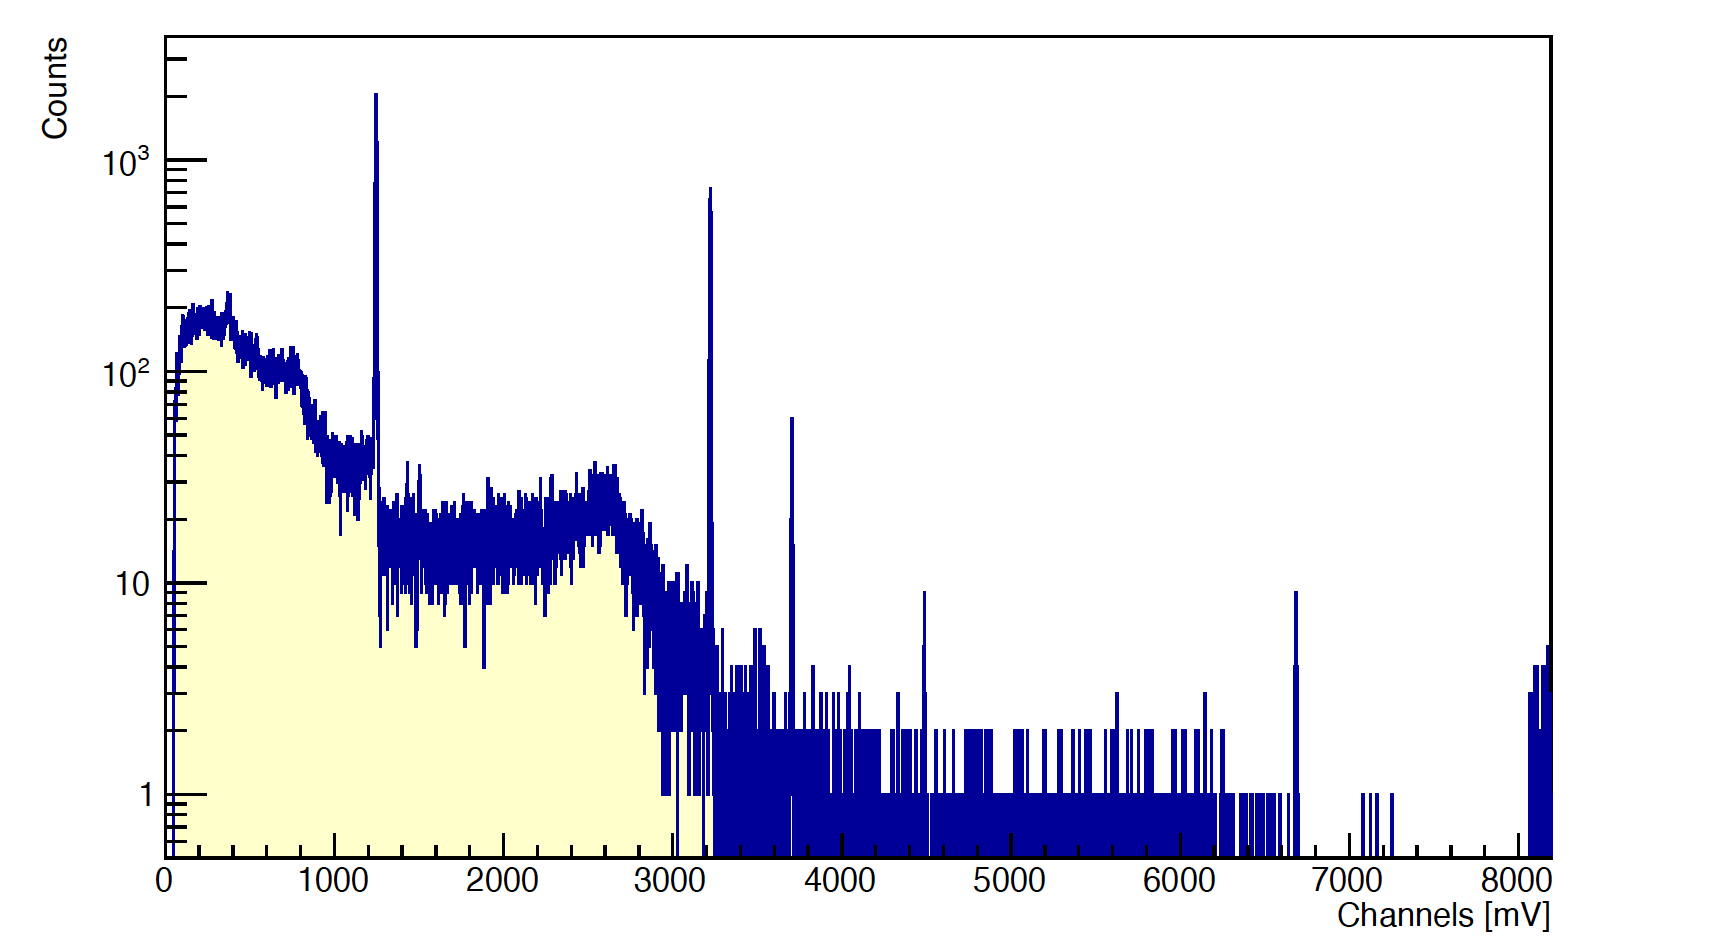
\includegraphics[scale=0.4]{img/sodioacqua}
    \caption{Spettro del sodio con acqua in scala logaritmica (4 cm)}
\end{figure}

\begin{figure}[!h]
    \centering
    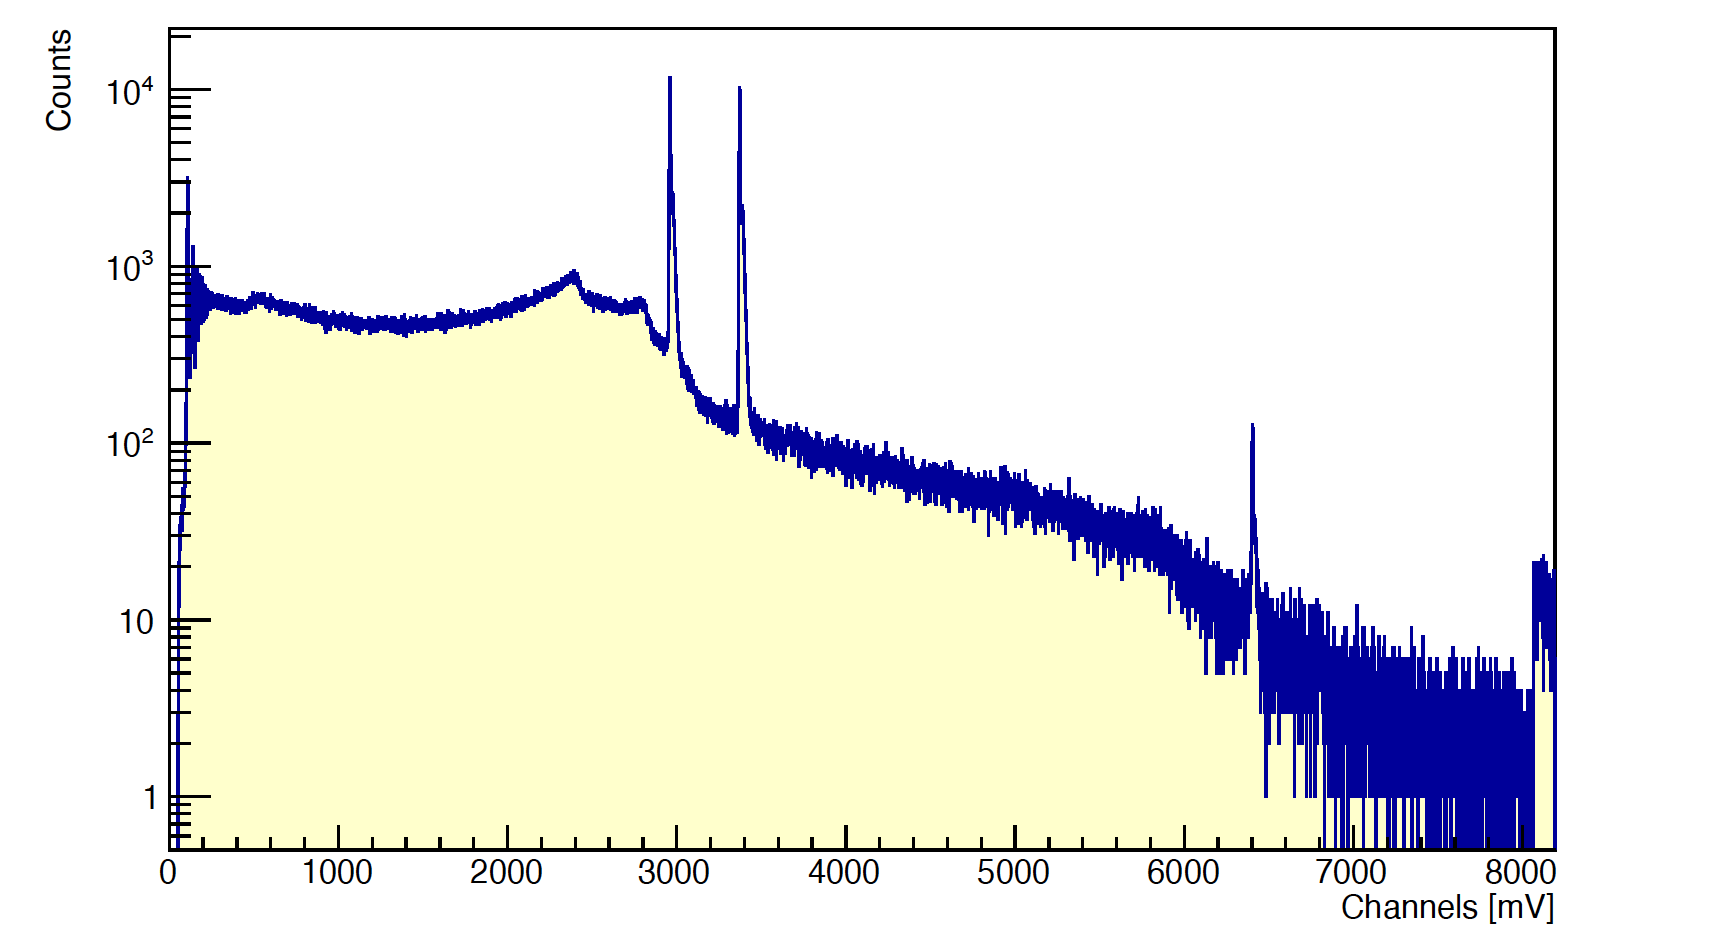
\includegraphics[scale=0.4]{img/cobaltorame}
    \caption{Spettro del colbalto con rame in scala logaritmica (11 cm)}
\end{figure}

\newpage

\begin{figure}[!h]
    \centering
    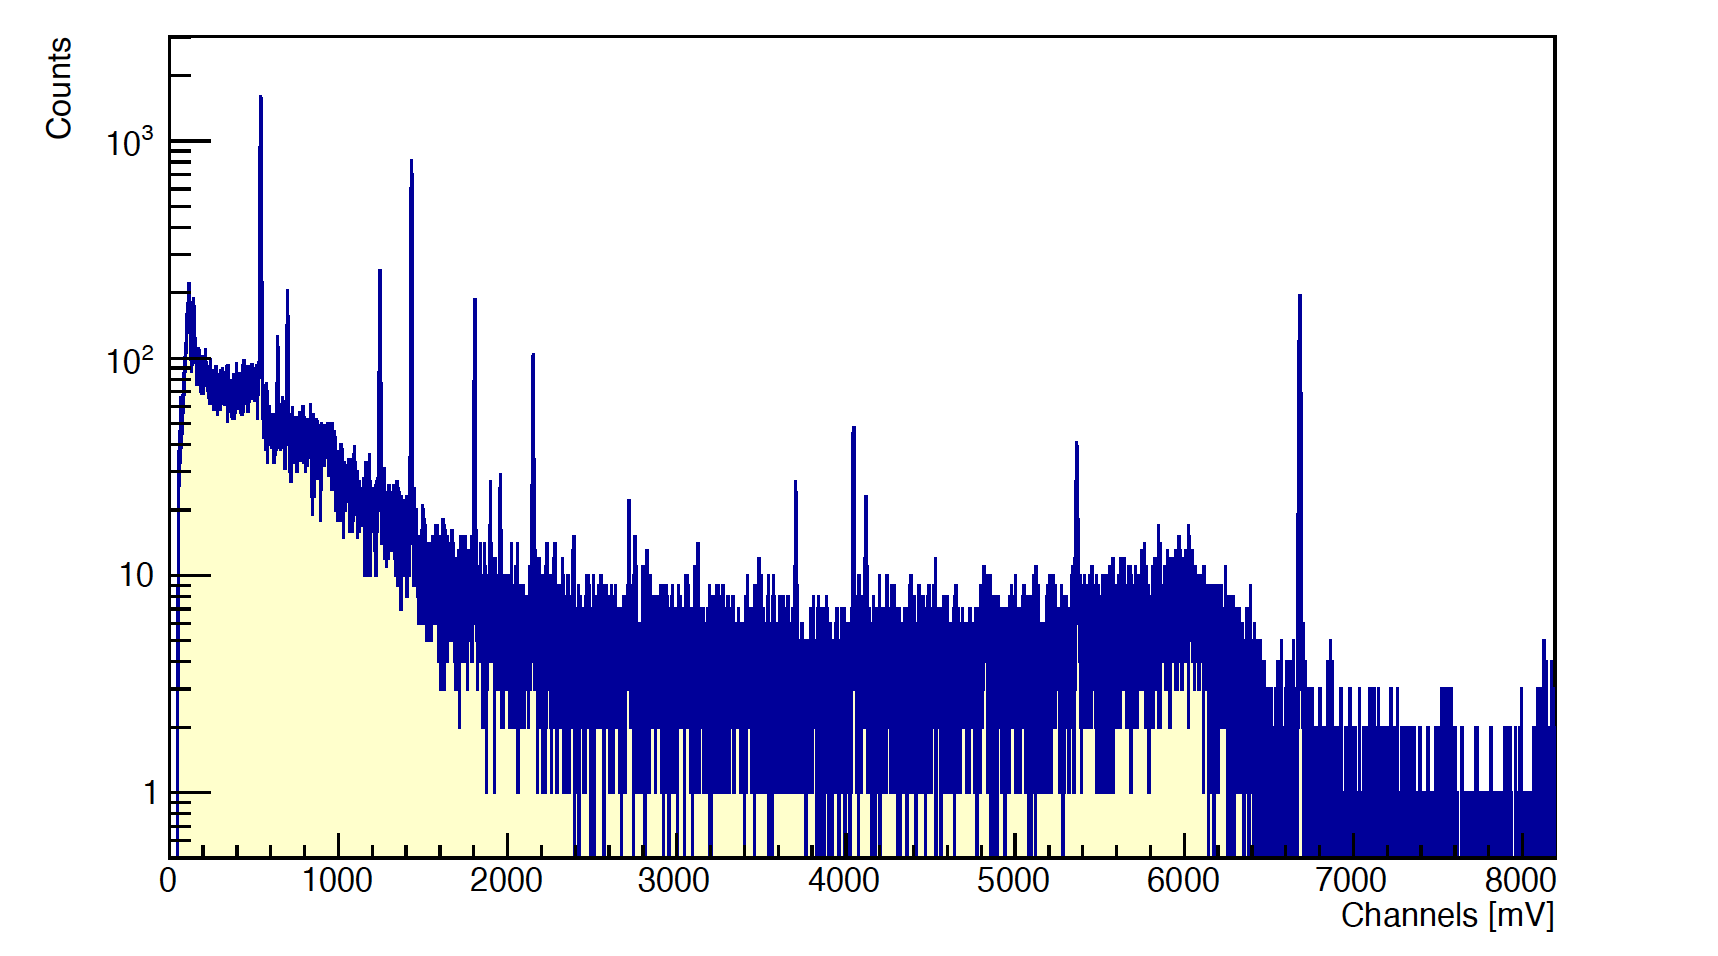
\includegraphics[scale=0.4]{img/toriopiombo}
    \caption{Spettro del torio con piombo in scala logaritmica (1 cm)}
\end{figure}

\noindent Per ogni picco visibile dei vari spettri, si procede ad individuare l'area sottesa al picco.  In accordo con la relazione (1), all'aumentare dello spessore di materiale da attraversare il numero di gamma che arrivano al rivelatore sar\`a sempre minore, e di conseguenza sar\`a minore l'area sottesa alla gaussiana. Riportiamo di seguito alcuni esempi, i restanti vengono riportati in appendice:

\begin{figure}[!h]
    \centering
    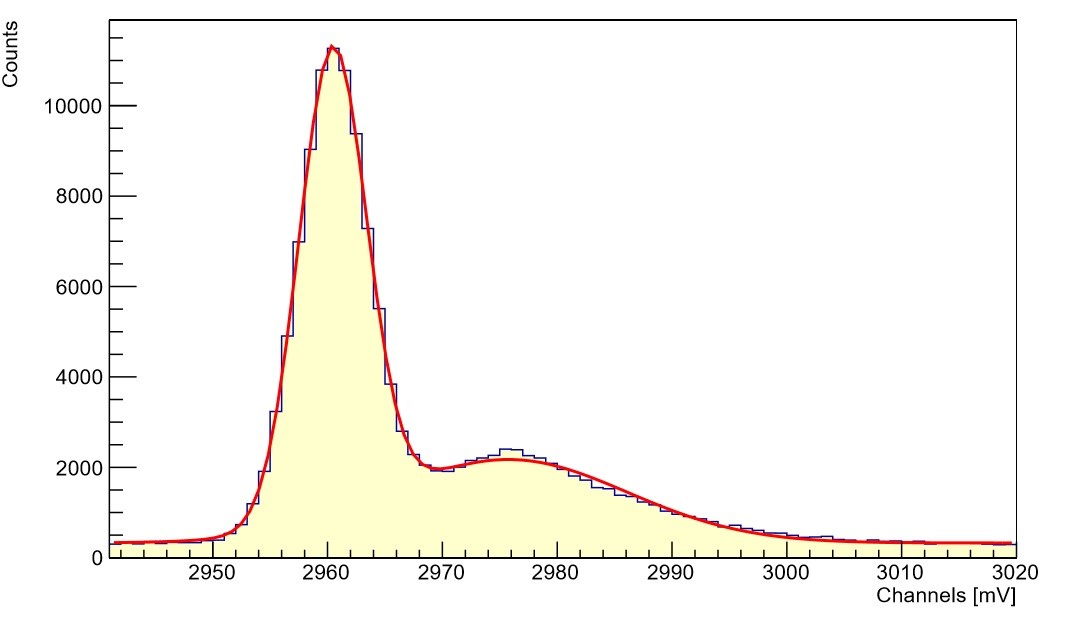
\includegraphics[scale=0.6]{grafici/piccocobalto}
    \caption{Esempio di picco della sorgente di 60Co}
\end{figure}

\begin{figure}[!h]
    \centering
    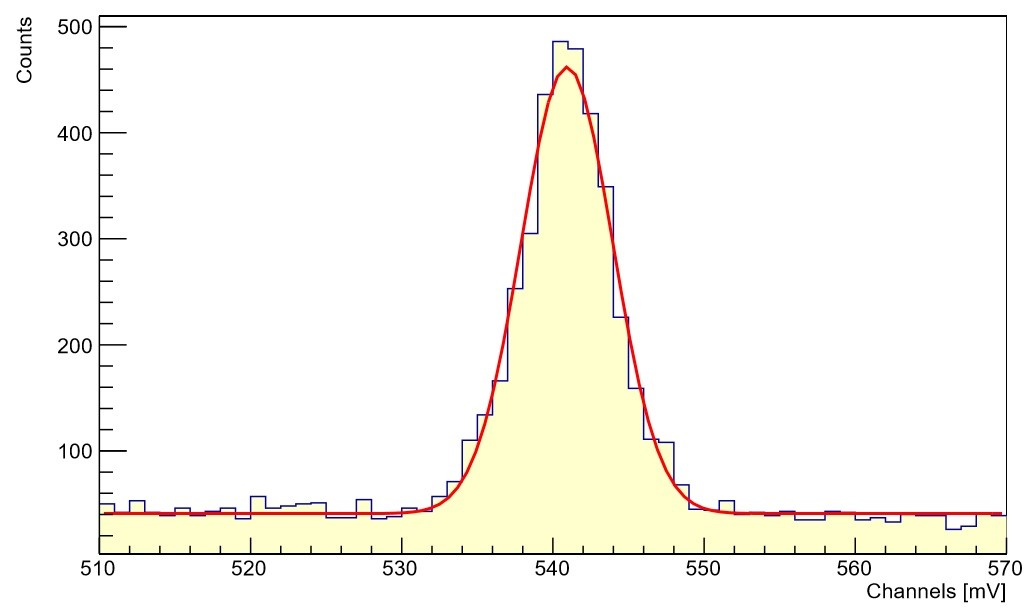
\includegraphics[scale=0.6]{grafici/piccotorio}
    \caption{Esempio di picco della sorgente di 228Th}
\end{figure}

\noindent L'interpolazione del picco \`e stata fatta con la somma di una gaussiana e di un polinomio di grado 0, che modellizza il fondo. In diversi casi, come nella Figura 4, \`e stato necessario interpolare con una seconda gaussiana. L'area rilevante ai fini dell'esperienza \`e solo quella della gaussiana principale: per individuarla \`e stato calcolaro l'integrale sotteso ad una gaussiana con i parametri di quella principale, ottenuti dal fit complessivo. Tenendo conto che le misure sono durate 6 minuti per quanto riguarda l'acqua e 2 minuti per rame e piombo, tramite la seguente relazione si procede a calcolare il rate di conteggi al secondo:

\begin{equation}
	\textrm{Rate} = \frac{\textrm{Area}}{\textrm{Durata  misura}}
\end{equation}

\noindent Per calcolare il coefficiente di attenuazione lineare dei vari materiali alle varie energie, si costruisce un grafico del rate in funzione dello spessore. Per interpolare è stata utilizzata la relazione (1):

\begin{figure}[H]
    \centering
    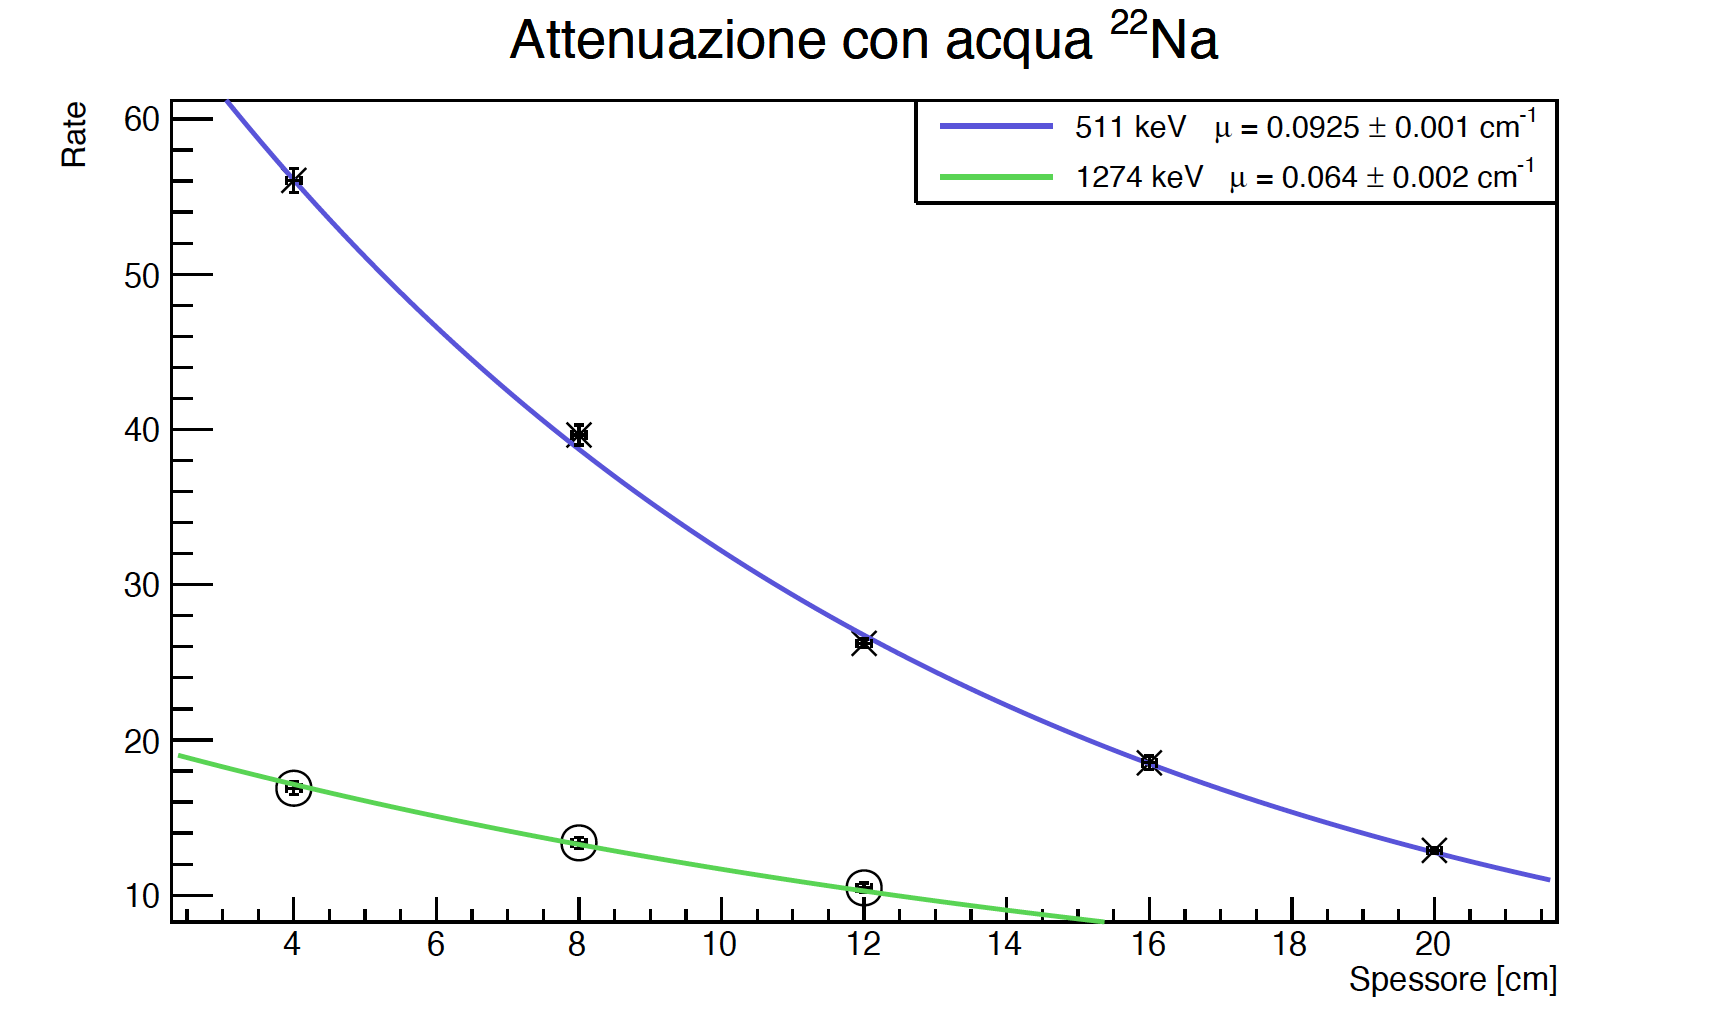
\includegraphics[scale=0.45]{grafici/attenuazionesodioacqua}
    \caption{Attenuazione del sodio in acqua}
\end{figure}

\begin{figure}[H]
    \centering
    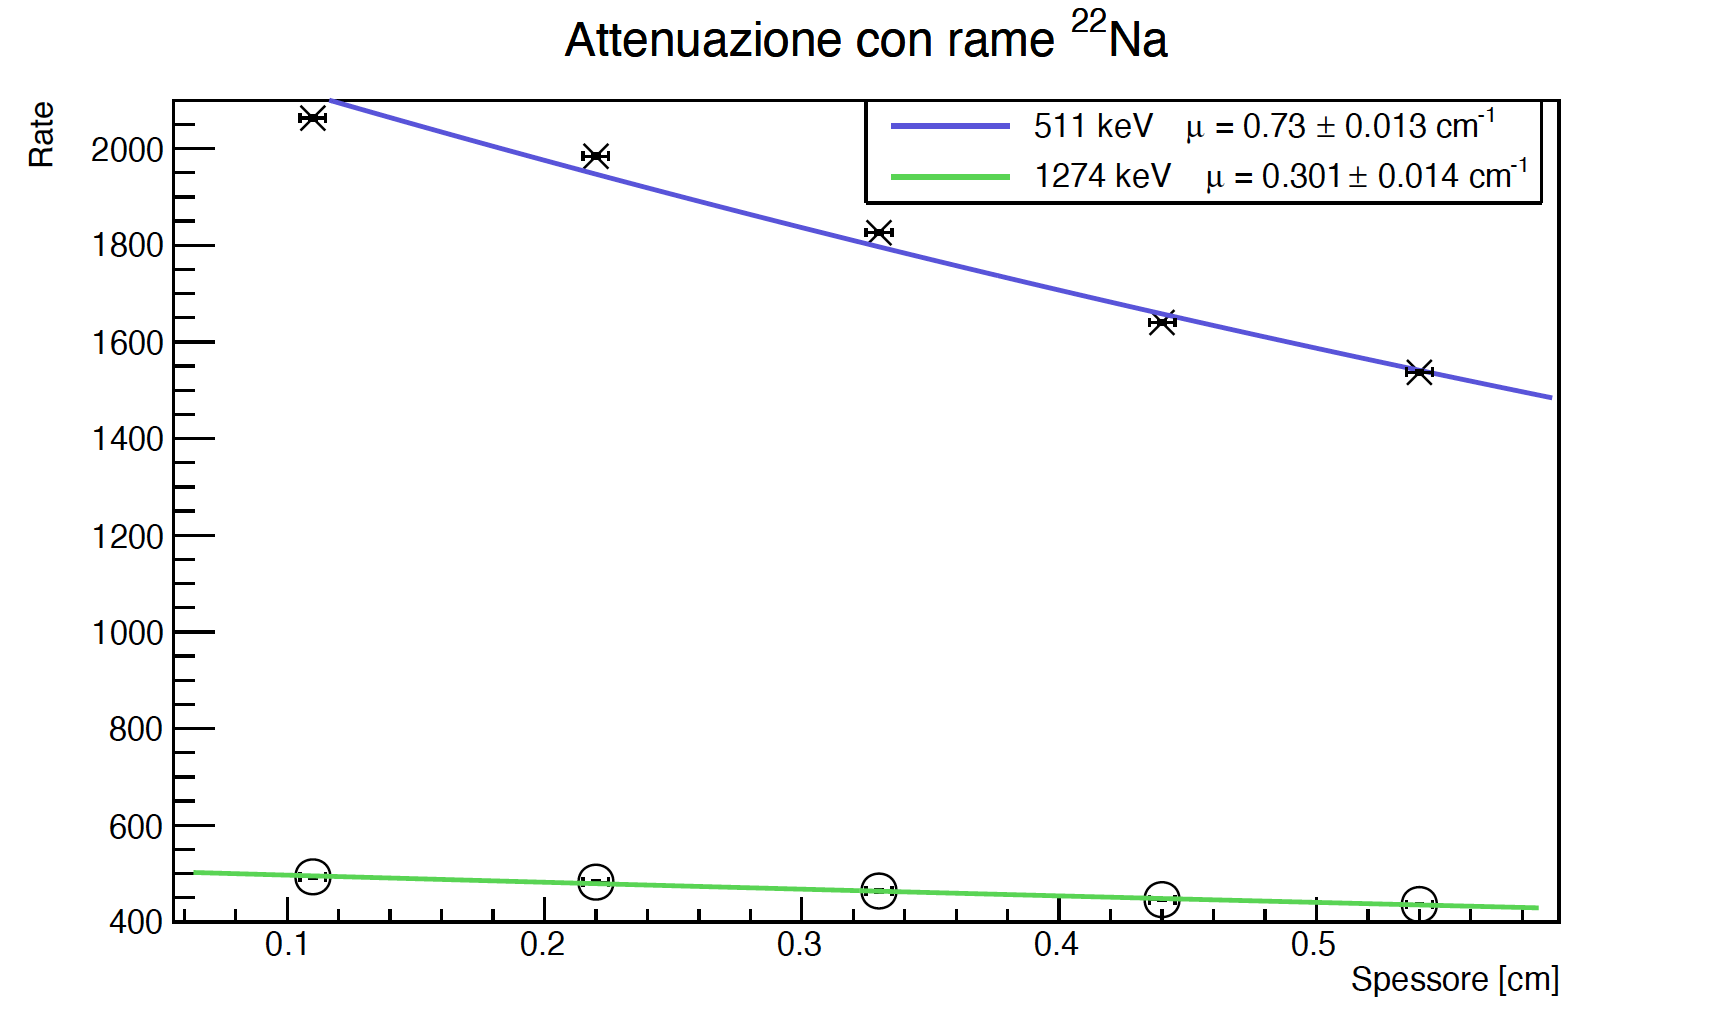
\includegraphics[scale=0.45]{grafici/attenuazionesodiorame}
    \caption{Attenuazione del sodio in rame}
\end{figure}

\begin{figure}[H]
    \centering
    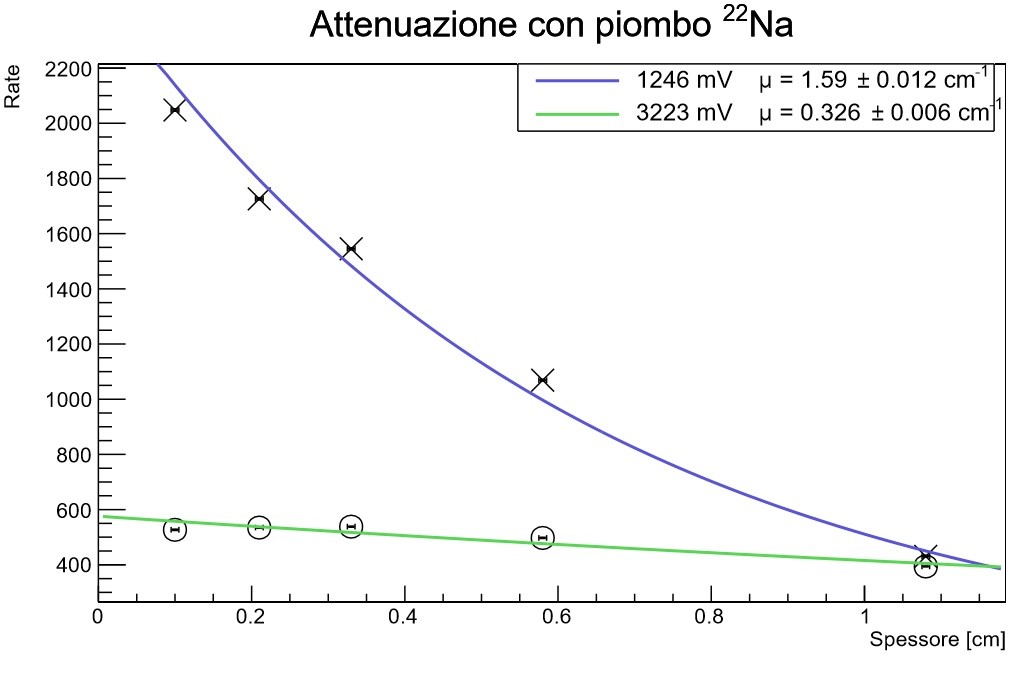
\includegraphics[scale=0.45]{grafici/attenuazionesodiopiombo}
    \caption{Attenuazione del sodio in piombo}
\end{figure}

\begin{figure}[H]
    \centering
    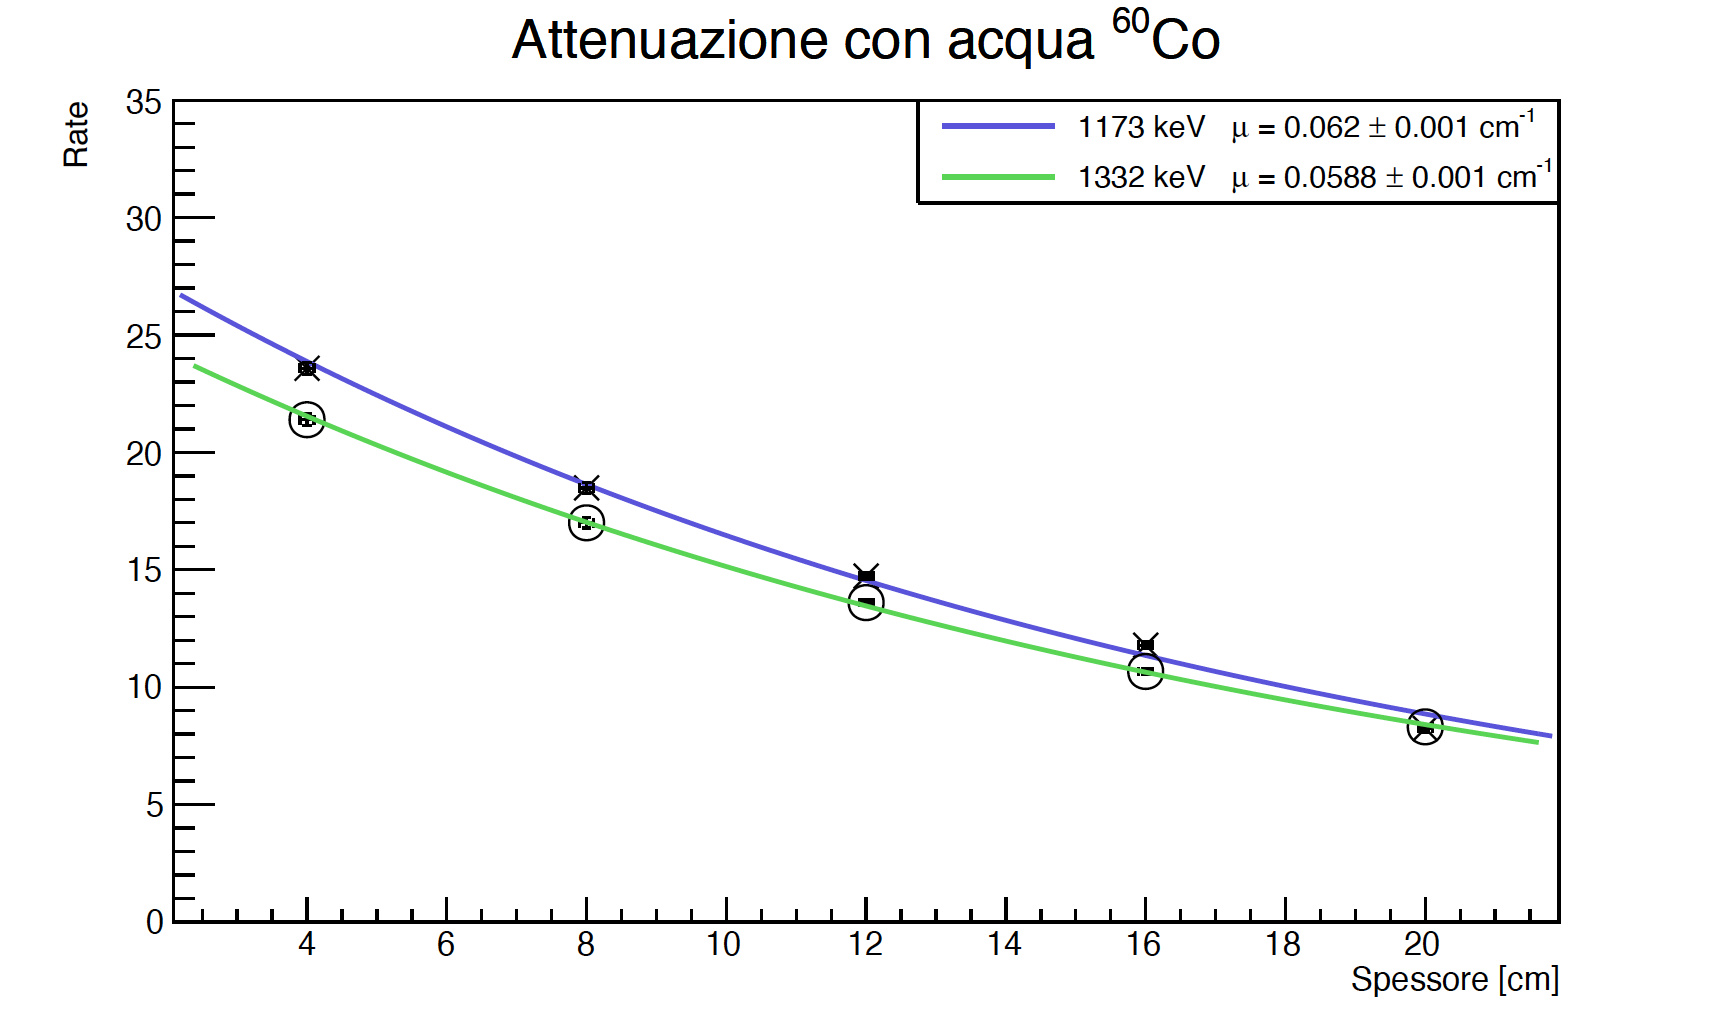
\includegraphics[scale=0.45]{grafici/attenuazionecobaltoacqua}
    \caption{Attenuazione del cobalto in acqua}
\end{figure}

\begin{figure}[H]
    \centering
    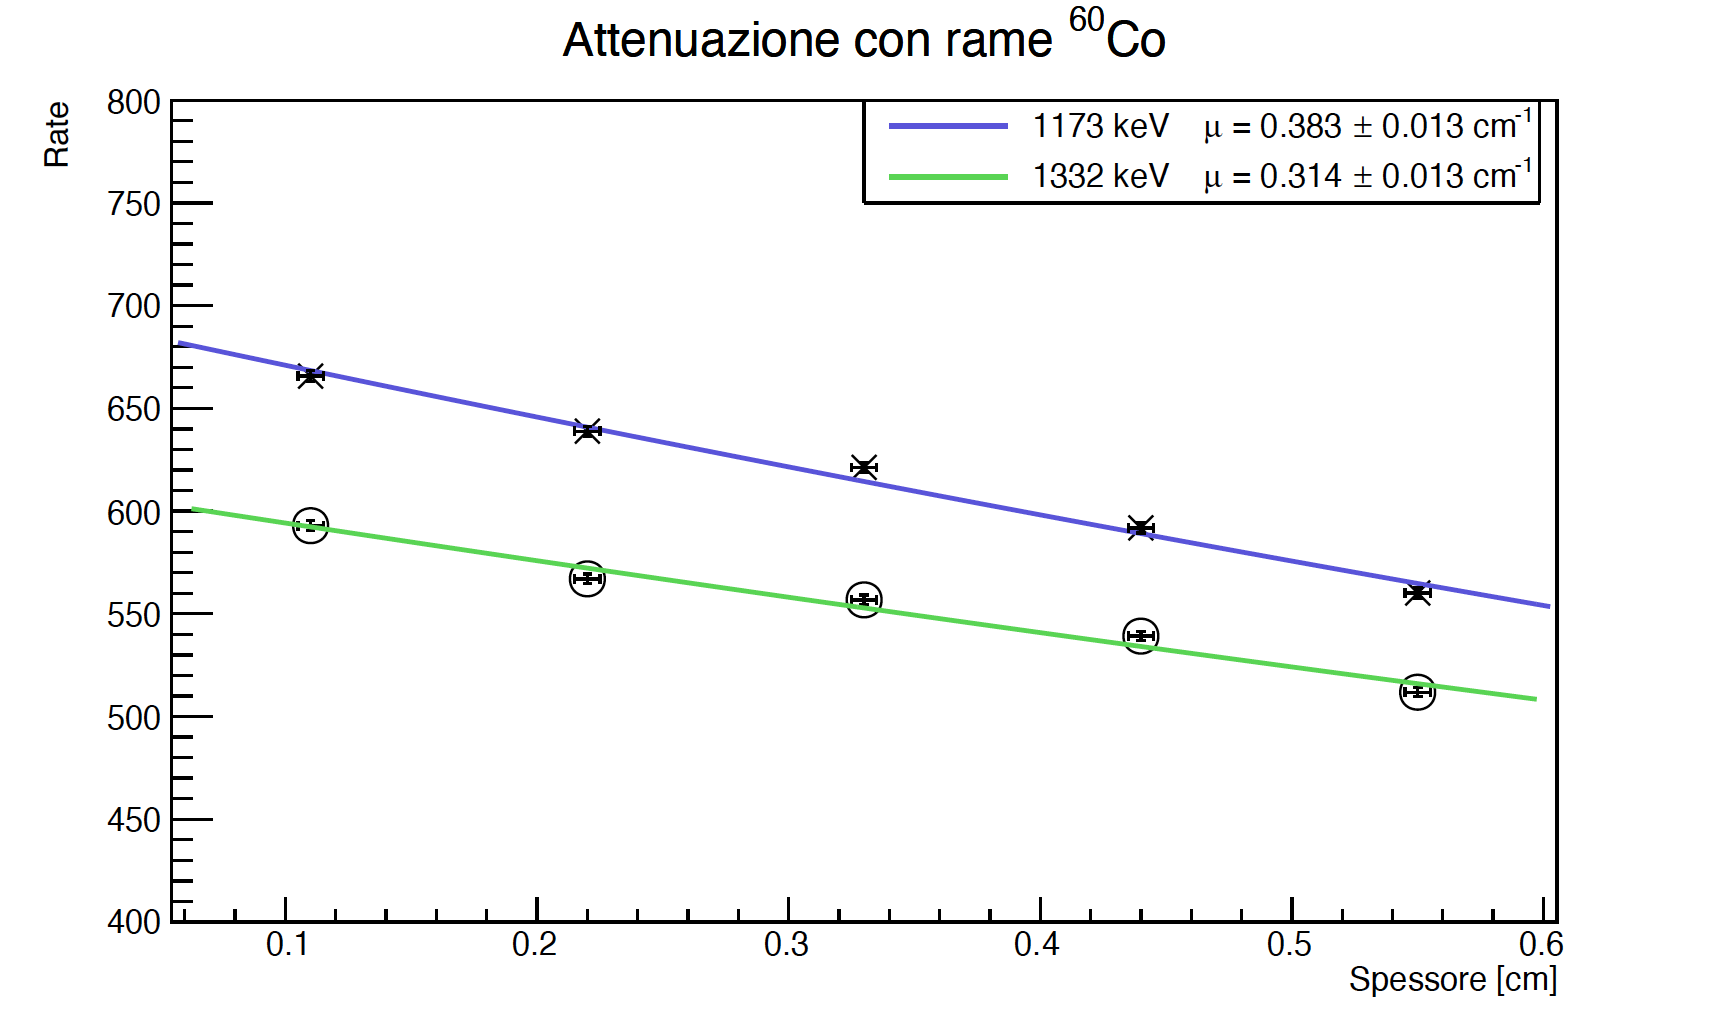
\includegraphics[scale=0.45]{grafici/attenuazionecobaltorame}
    \caption{Attenuazione del cobalto in rame}
\end{figure}

\begin{figure}[H]
    \centering
    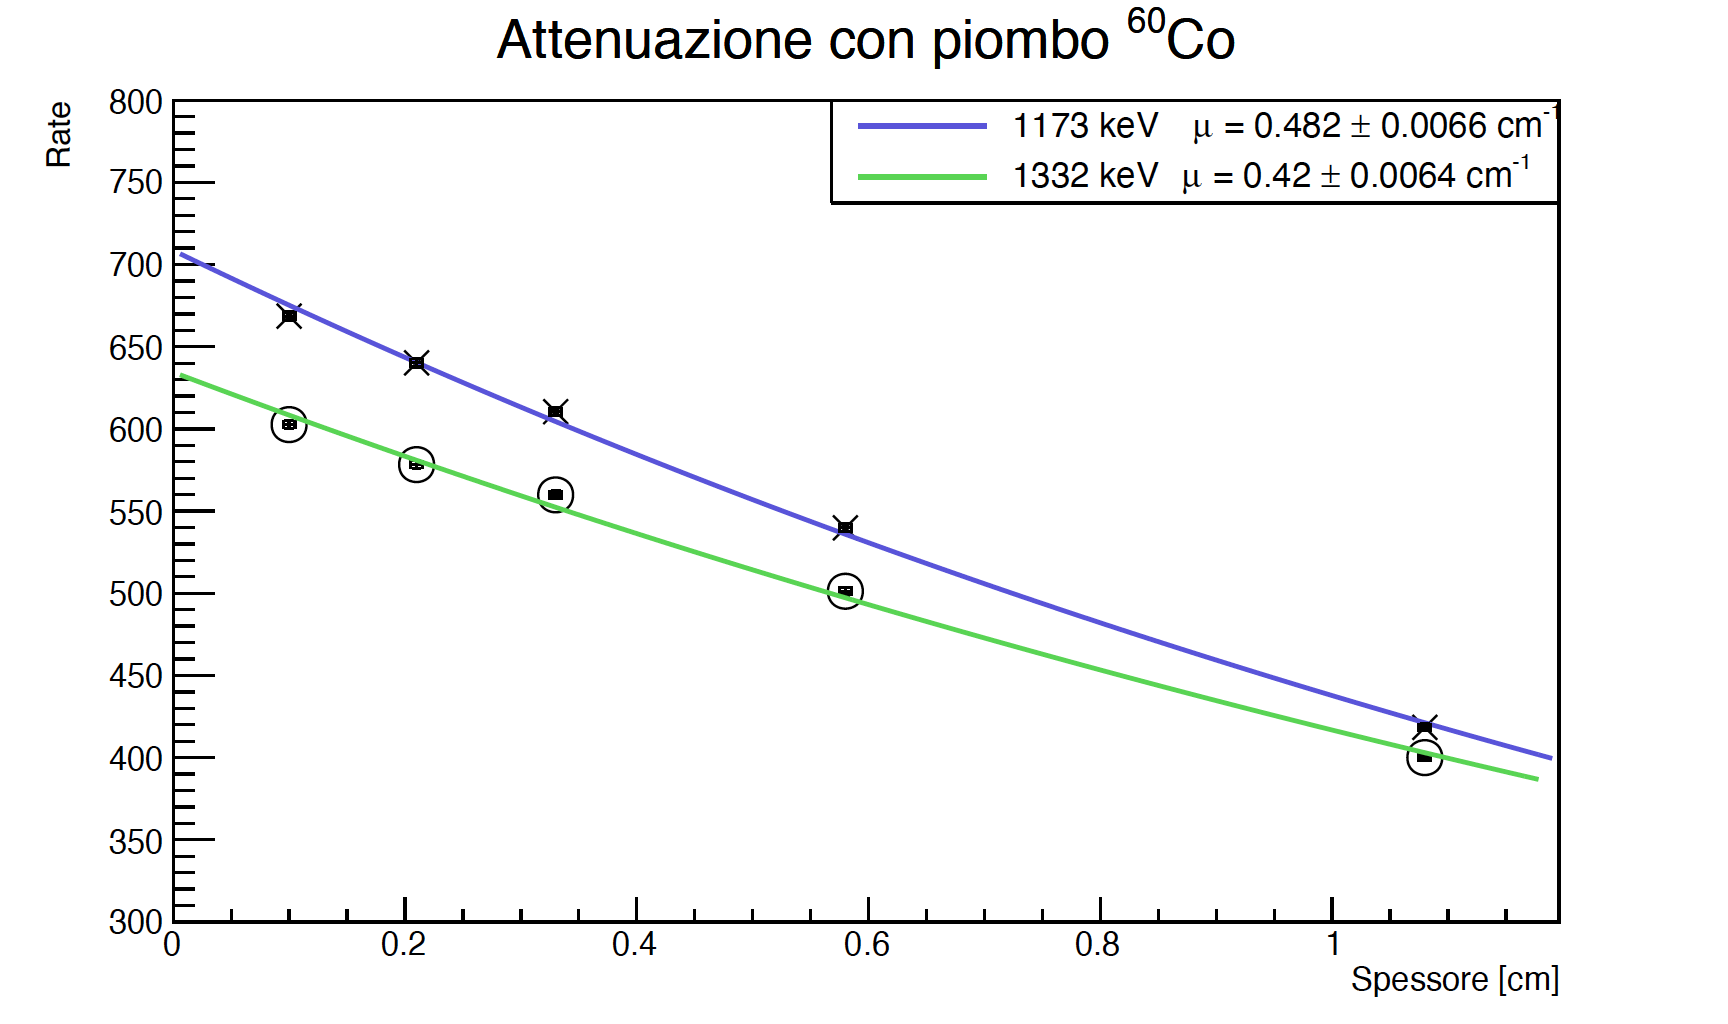
\includegraphics[scale=0.45]{grafici/attenuazionecobaltopiombo}
    \caption{Attenuazione del cobalto in piombo}
\end{figure}

\begin{figure}[H]
    \centering
    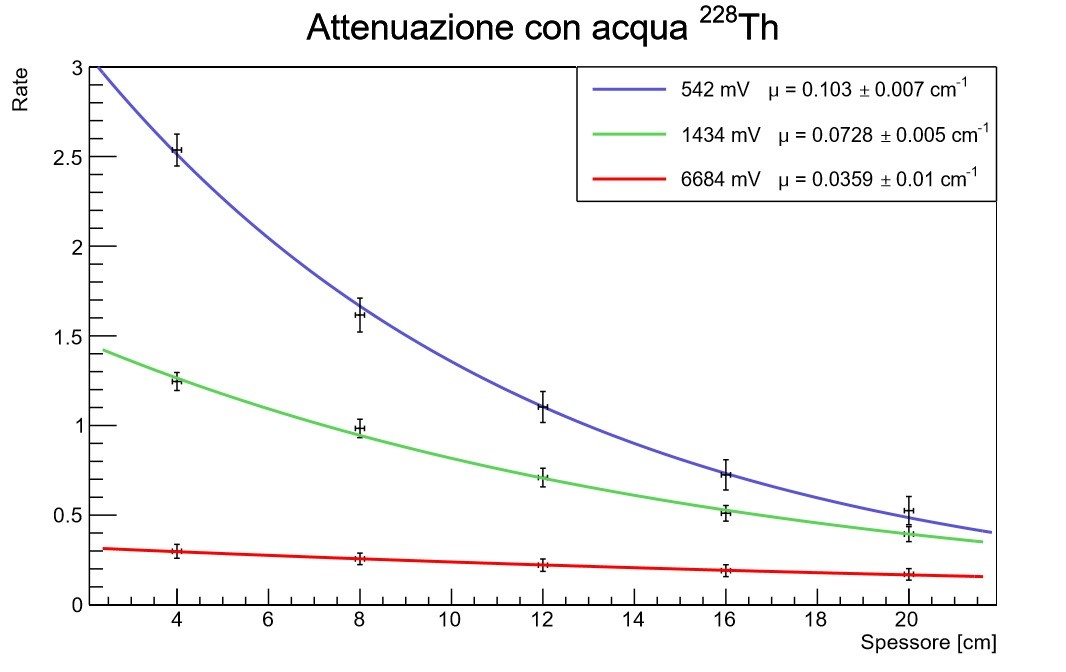
\includegraphics[scale=0.45]{grafici/attenuazionetorioacqua}
    \caption{Attenuazione del torio in acqua}
\end{figure}

\begin{figure}[H]
    \centering
    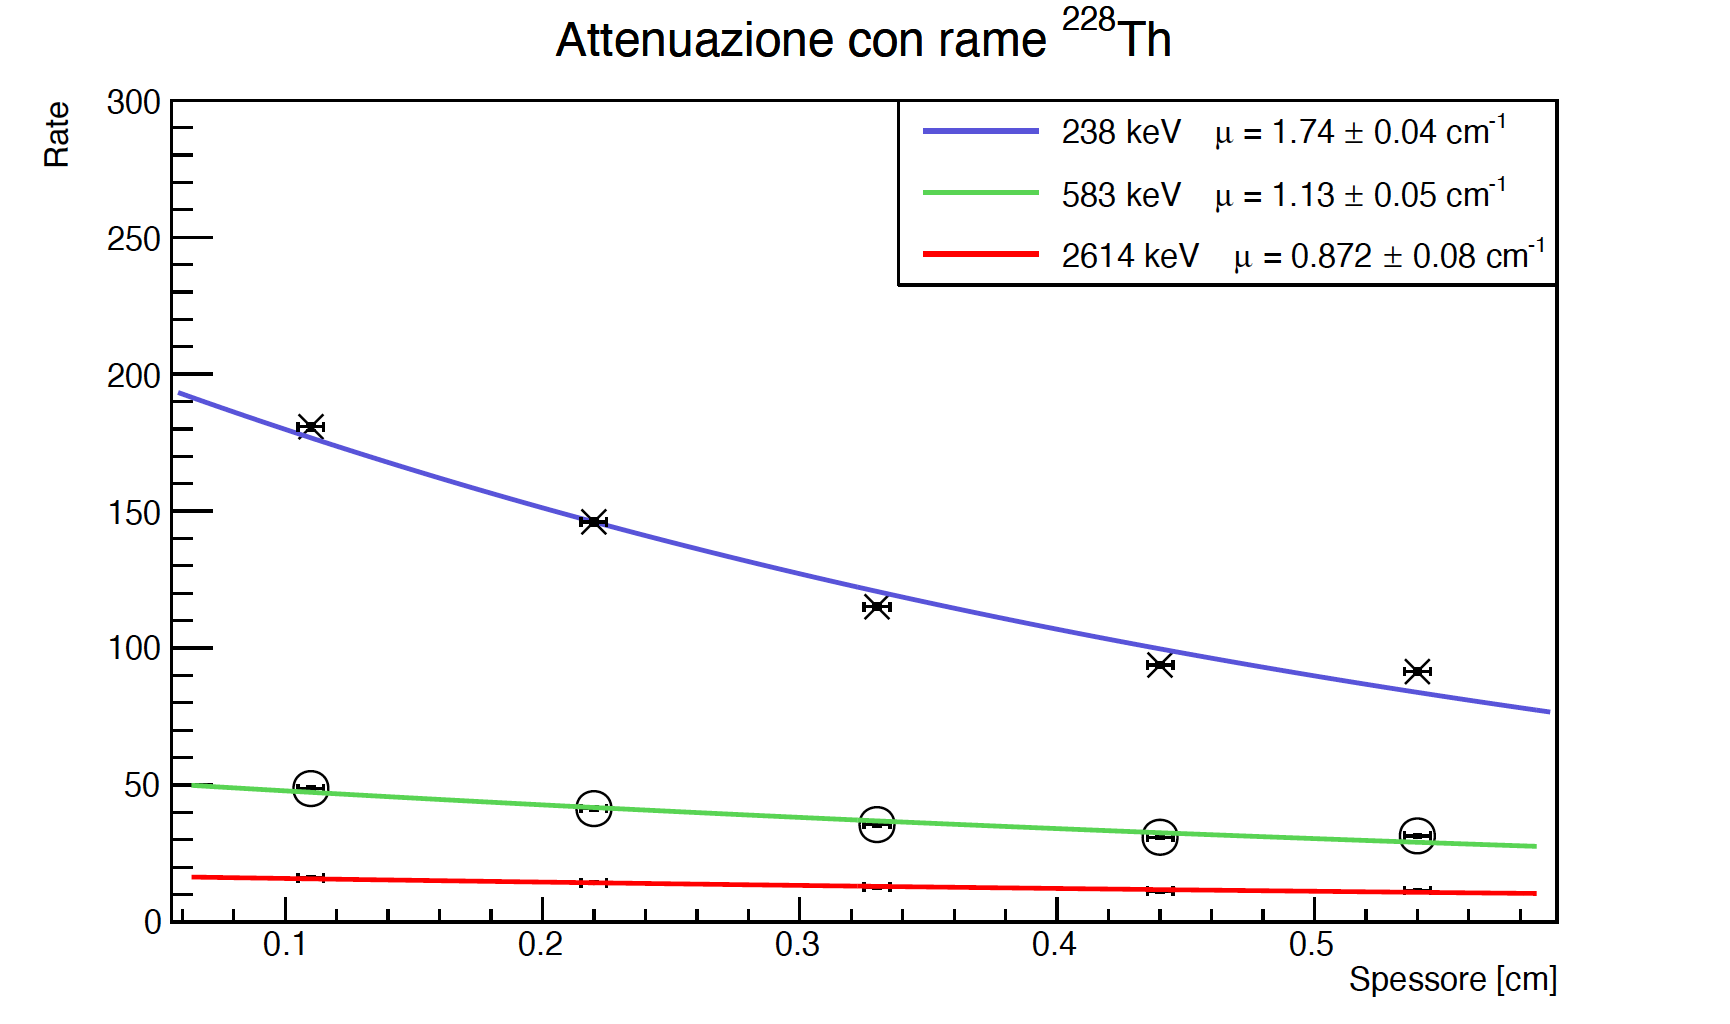
\includegraphics[scale=0.45]{grafici/attenuazionetoriorame}
    \caption{Attenuazione del torio in rame}
\end{figure}

\begin{figure}[H]
    \centering
    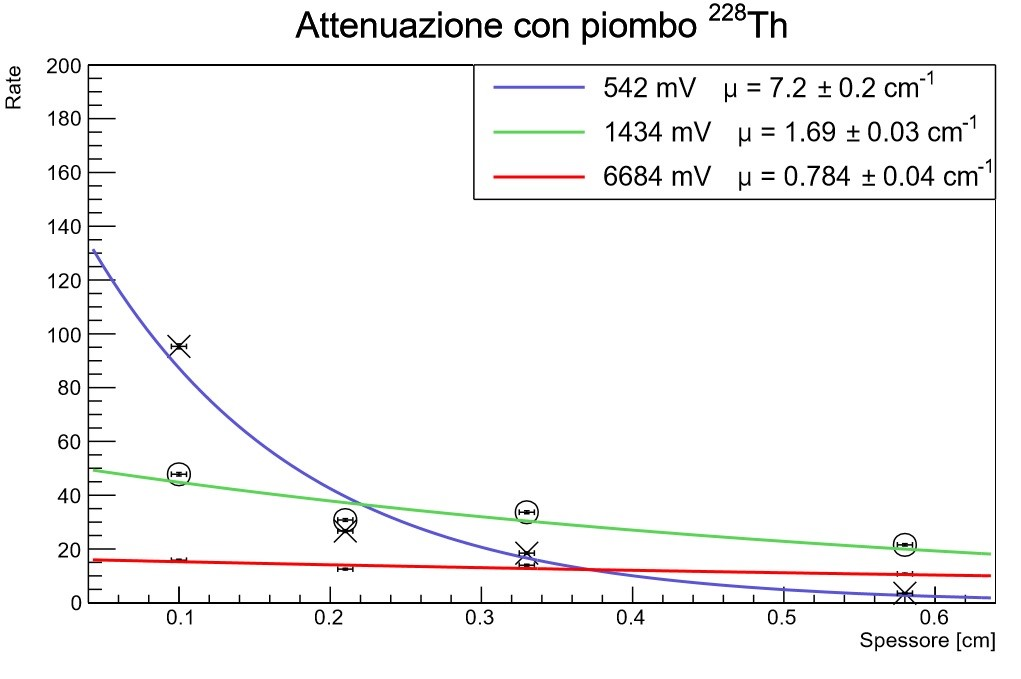
\includegraphics[scale=0.45]{grafici/attenuazionetoriopiombo}
    \caption{Attenuazione del torio in piombo}
\end{figure}

\noindent L'andamento ottenuto per i vari picchi \`e quello atteso: l'attenuazione segue un andamento esponenziale decrescente, caratterizzato dal coefficiente di attenuazione lineare specifico indicato nelle legende dei grafici.

\subsection{Picco a 1460 keV}

\noindent Negli spettri a nostra disposizione si nota la presenza di un picco non atteso, attorno ad una energia di 1460 keV. La presenza di questo picco \`e dovuta alla presenza di 40K nell'ambiente. Come fatto nel punto precendente, andiamo a calcolare il rate di conteggi al secondo di questo picco, mettendolo in funzione dello spessore del materiale:

\begin{figure}[H]
    \centering
    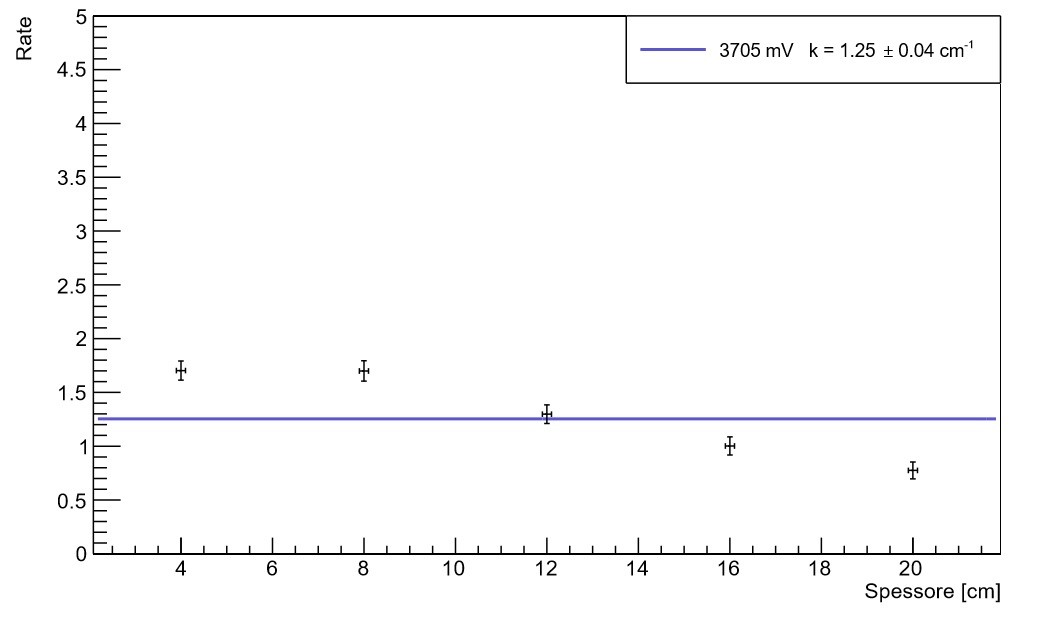
\includegraphics[scale=0.45]{grafici/1460keV}
    \caption{Andamento rate picco a 1460 keV}
\end{figure}

\noindent L'andamento riportato \`e relativo alla sorgente di torio con acqua come bersaglio. Il picco in questione risulta pi\`u evidente in alcuni spettri rispetto ad altri, dove il rate del fondo \`e paragonabile a quello del ${}^{40}$K, e l'andamento del picco di nostro interesse si confonde con il fondo stesso. Si nota come il rate del ${}^{40}$K sia pressoch\`e costante: questo \`e dovuto al fatto che, essendo questo picco dovuto alla radioattivit\`a ambientale, non è prodotto dalla sorgente in questione e di conseguenza non deve attraversare il materiale venendo attenuato. Dunque, per misure della stessa durata temporale il numero di conteggi al secondo di questo isotopo sarà costante.

\subsection{Coefficiente di attenuazione massico e sezione d'urto}
Avendo a disposizione i coefficienti di attenuazione lineare $\mu$ ricavati nella sezione 3.1, andiamo a calcolare i coefficienti di attenuazione massici $\mu/\rho$. Per i 3 materiali si utilizzano come densit\`a:

$$
	\rho_{acqua} = 1\, \unit{g/cm^3}
$$
$$
	\rho_{rame} = 8,96\, \unit{g/cm^3}
$$
$$
	\rho_{piombo} = 11,34\, \unit{g/cm^3}
$$

\noindent I risultati ottenuti vengono messi in un grafico in funzione dell'energia, ottenendo in totale 3 grafici, uno per ciascun materiale bersaglio. Come sottolineato nell'introduzione, attraverso la relazione (2), la sezione d'urto \`e proporzionale a $\mu/\rho$. In questi 3 grafici, avendo fissato di volta in volta il materiale, la sezione d'urto \`e ottenuta semplicemente moltiplicando i valori ottenuti per un valore costante $A/N_{Av}$; per questo l'andamento in funzione dell'energia pu\`o essere ricavato semplicemente dal grafico del coefficiente di attenuazione massico.

\subsubsection{Acqua}
Riportiamo di seguito il grafico di $\mu/\rho$ in funzione dell'energia per l'acqua:

\begin{figure}[H]
    \centering
    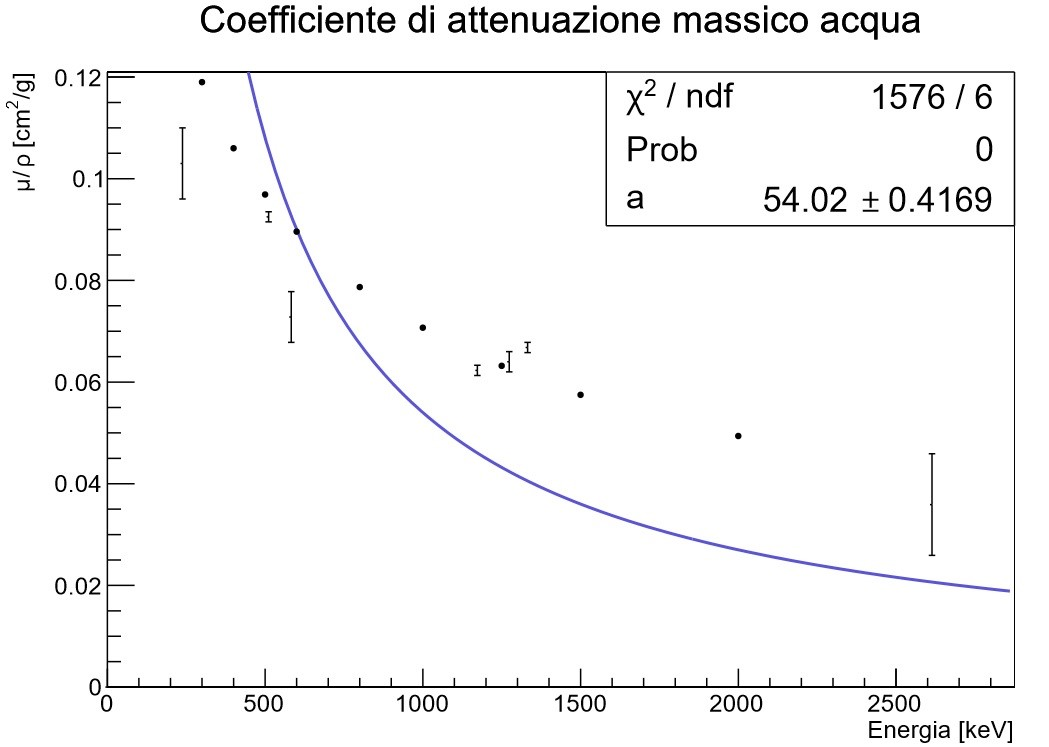
\includegraphics[scale=0.6]{grafici/massicoacqua}
    \caption{Coefficiente di attenuazione massico per acqua}
\end{figure}

\noindent Il grafico \`e stato interpolato, tenendo conto delle relazioni (3), (4) e (5), con la seguente funzione:

\begin{equation}
	\sigma = \frac{a}{E}
\end{equation}
\noindent poich\`e, nel range di energie considerate, in acqua, prevale lo scattering Compton. Nel grafico \`e riportato anche l'andamento teorico del coefficiente di attenuazione massico, rappresentato dai pallini. Si pu\`o notare come, appunto, prevalga l'effetto Compton in questo range di energie, seppur i dati sperimentali non siano completamente conformi alla teoria. Ci\`o \`e dovuto principalmente ad una sottostima del coefficiente $\mu$ a determinate energie, difficolt\`a ascrivibile al calcolo delle corrette aree sottese ai picchi nei vari spettri.  

\subsubsection{Rame}
Riportiamo di seguito il grafico di $\mu/\rho$ in funzione dell'energia per il rame:

\begin{figure}[H]
    \centering
    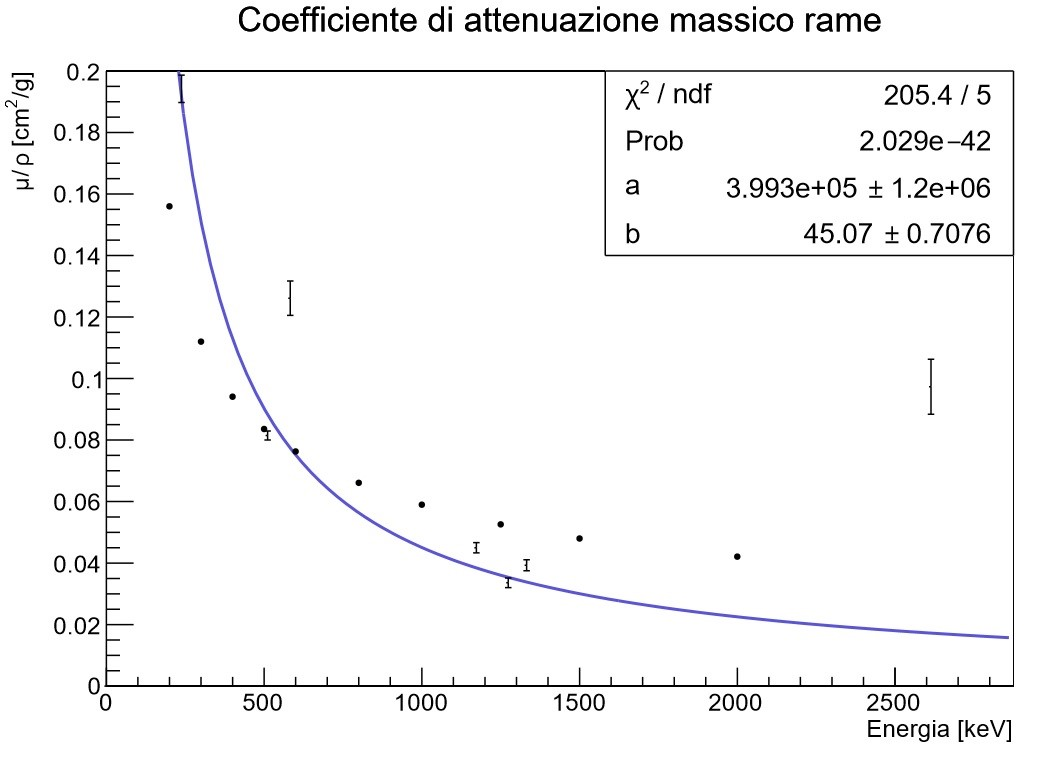
\includegraphics[scale=0.6]{grafici/massicorame}
    \caption{Coefficiente di attenuazione massico per rame}
\end{figure}

\noindent Il grafico \`e stato interpolato, tenendo conto delle relazioni (3), (4) e (5), con la seguente funzione:

\begin{equation}
	\sigma = \frac{a}{E^{3.5}} + \frac{b}{E}
\end{equation}
\noindent poich\`e, nel range di energie considerate prevale l'effetto Compton, ma avendo il rame uno Z=29 anche l'effetto fotoelettrico comincia ad essere rilevante. In particolar modo l'effetto fotoelettrico \`e importante a basse energie, mentre crescendo in energia nel caso del rame continua ad essere preponderante il Compton. Anche in questo caso, alcuni punti si discostano in modo importante dall'andamento teorico.

\subsubsection{Piombo}
Riportiamo di seguito il grafico di $\mu/\rho$ in funzione dell'energia il piombo:

\begin{figure}[H]
    \centering
    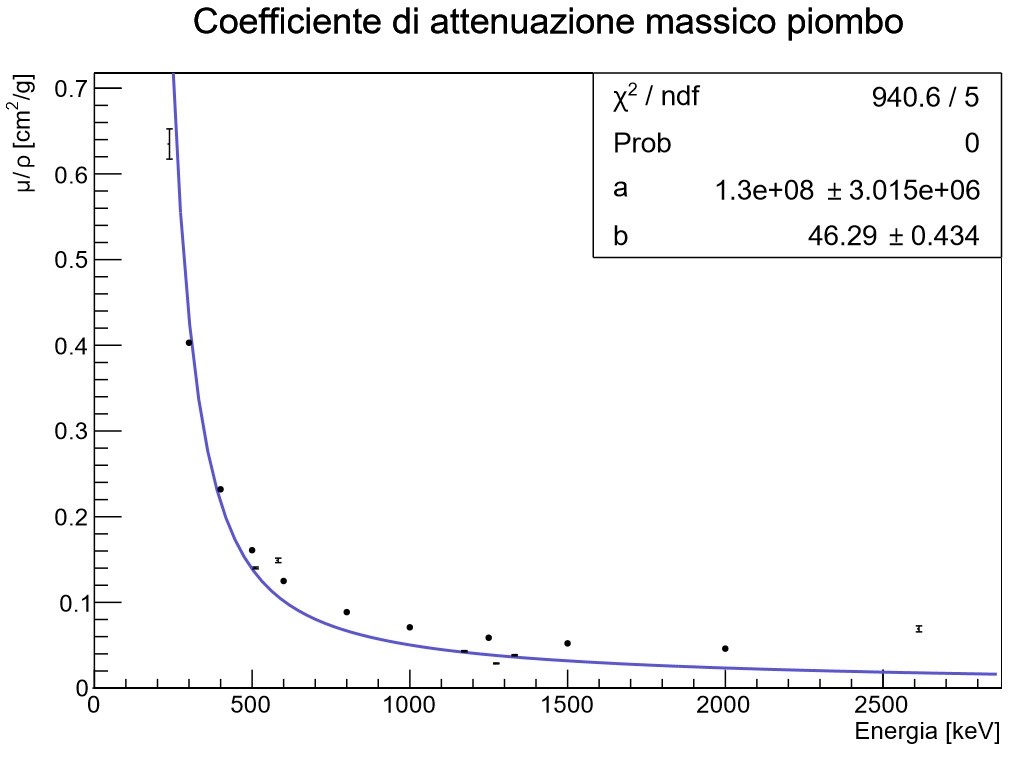
\includegraphics[scale=0.6]{grafici/massicopiombo}
    \caption{Coefficiente di attenuazione massico per piombo}
\end{figure}

\noindent Il grafico \`e stato interpolato, tenendo conto delle relazioni (3), (4) e (5), con la seguente funzione:

\begin{equation}
	\sigma = \frac{a}{E^{3.5}} + \frac{b}{E}
\end{equation}
In questo caso stiamo utilizzando un materiale con Z=82, molto elevato. Per questo, a basse energie l'effetto fotoelettrico si pu\`o notare come sia preponderante, mentre al crescere dell'energia diventa sempre p\`u importante il Compton dato che il termine al denominatore nella relazione diventa sempre pi\`u significativo.

\subsection{Sezione d'urto in funzione di Z}
In questo caso ci proponiamo invece di studiare la dipendenza dalla Z del materiale della sezione d'urto. Fissata l'energia di un certo picco, andiamo a calcolare la sezione d'urto attraverso la relazione (2). Come A \`e stata utilizzata la massa molecolare dell'acqua e la massa atomica di rame e piombo, pesata in base all'abbondanza dei vari isotopi. Per ogni picco avremo a disposizione 3 valori, ognuno corrispondente ad uno dei 3 materiali usati come bersaglio. Si ottengono i seguenti grafici:

\begin{figure}[H]
    \centering
    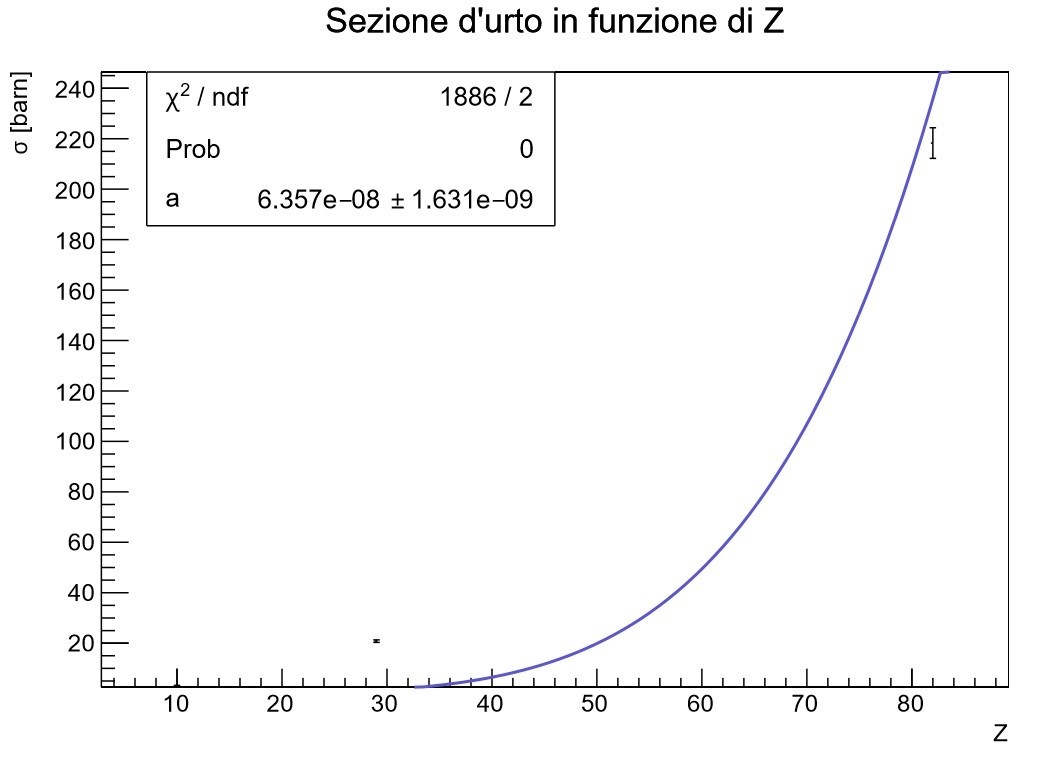
\includegraphics[scale=0.6]{grafici/picco238}
    \caption{Picco a 238 keV}
\end{figure}

\begin{figure}[H]
    \centering
    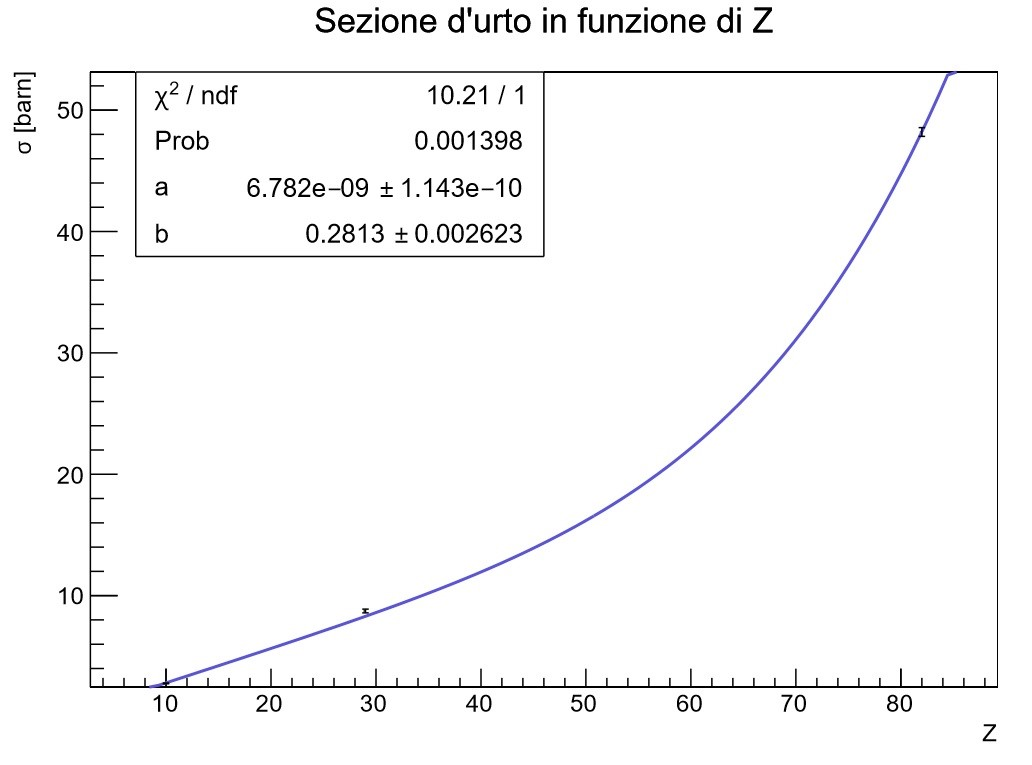
\includegraphics[scale=0.6]{grafici/picco511}
    \caption{Picco a 511 keV}
\end{figure}

\begin{figure}[H]
    \centering
    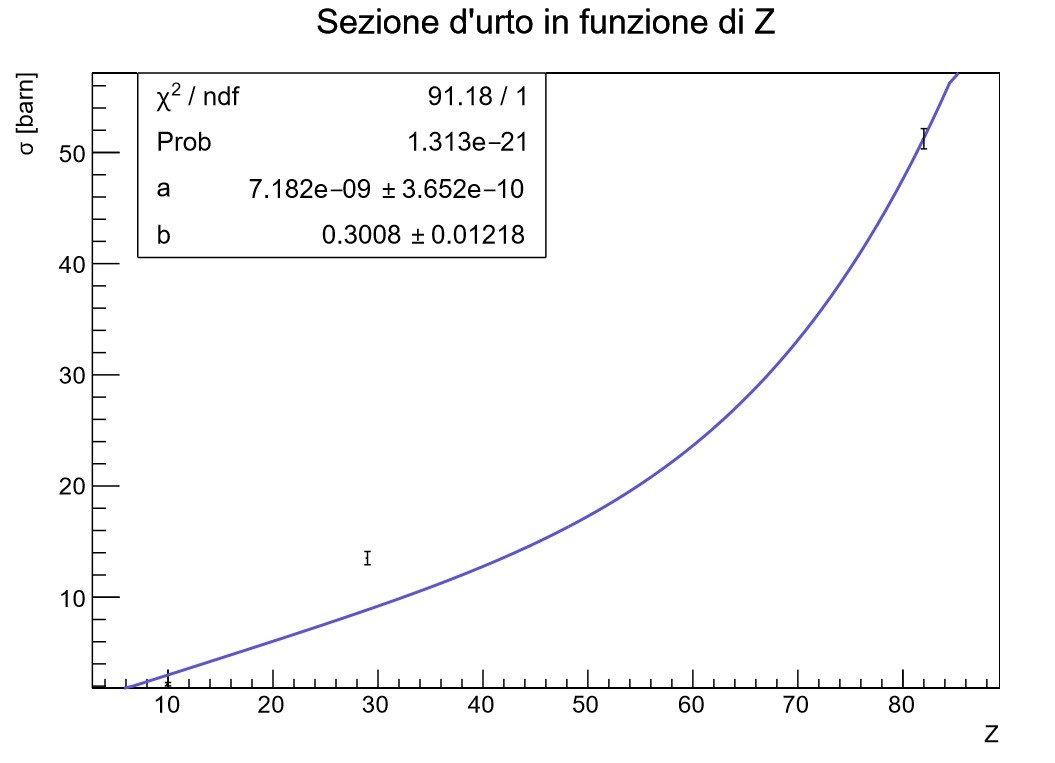
\includegraphics[scale=0.6]{grafici/picco583}
    \caption{Picco a 583 keV}
\end{figure}

\begin{figure}[H]
    \centering
    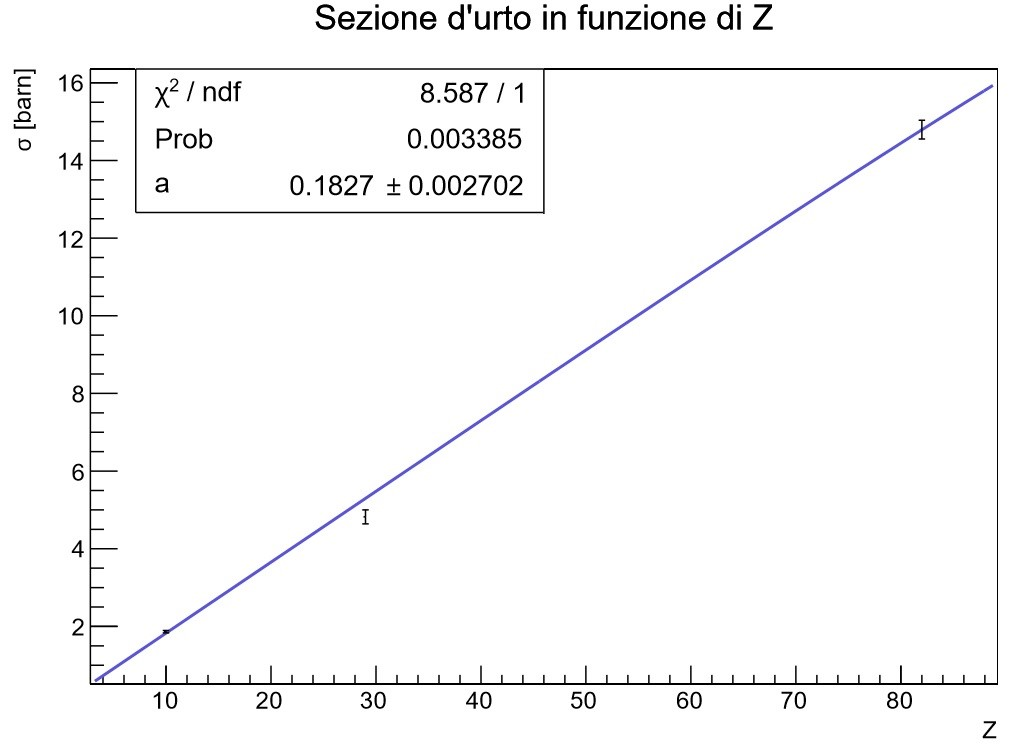
\includegraphics[scale=0.6]{grafici/picco1173}
    \caption{Picco a 1173 keV}
\end{figure}

\begin{figure}[H]
    \centering
    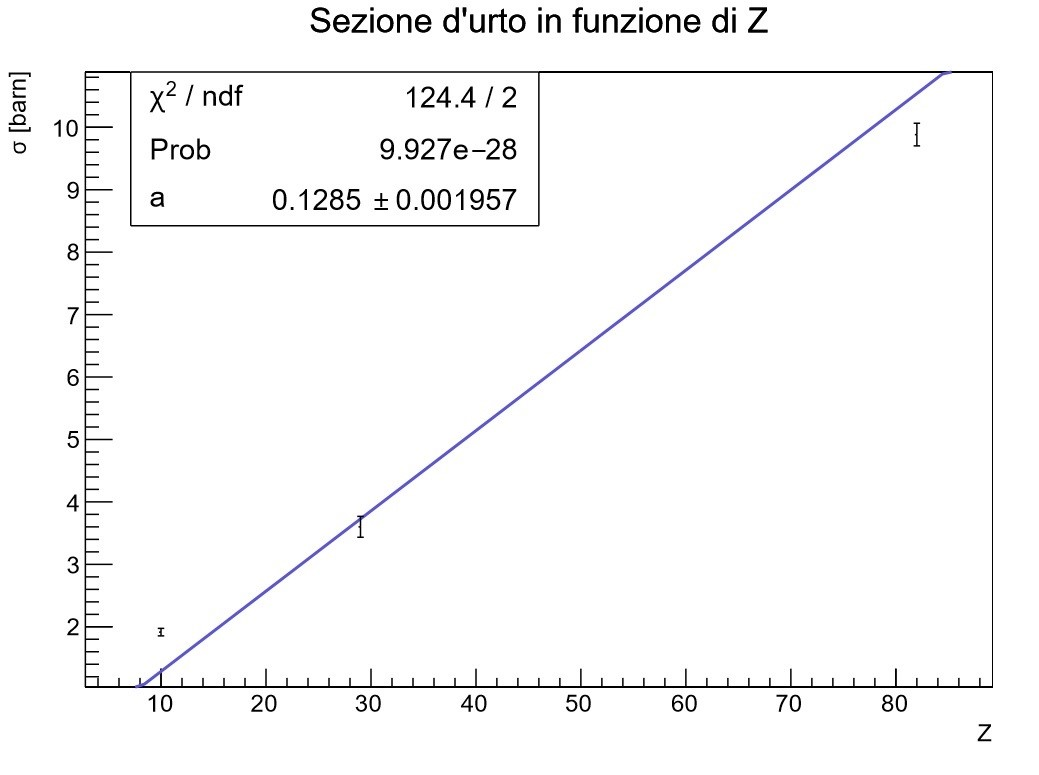
\includegraphics[scale=0.6]{grafici/picco1274}
    \caption{Picco a 1274 keV}
\end{figure}

\begin{figure}[H]
    \centering
    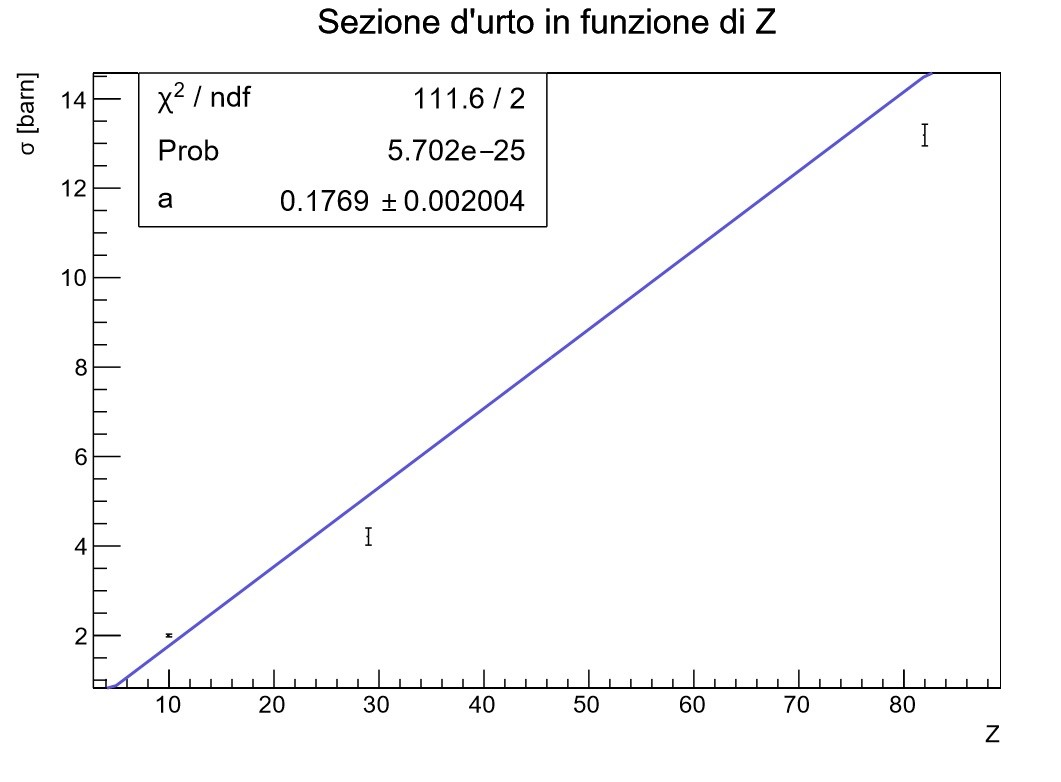
\includegraphics[scale=0.6]{grafici/picco1332}
    \caption{Picco a 1332 keV}
\end{figure}

\begin{figure}[H]
    \centering
    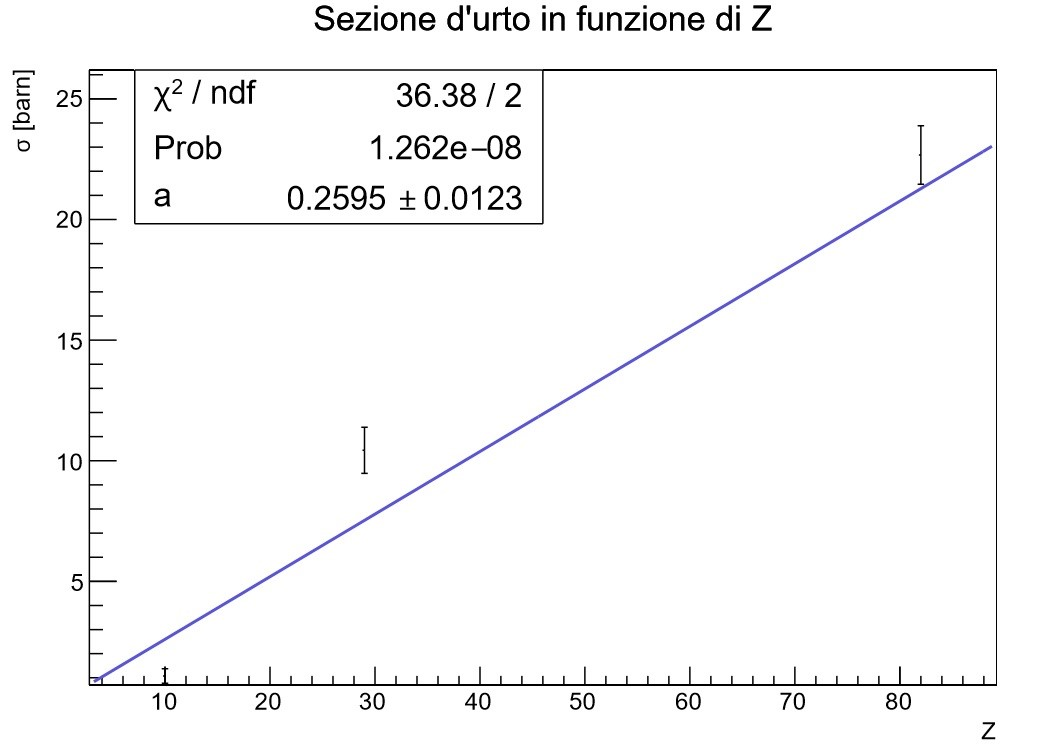
\includegraphics[scale=0.6]{grafici/picco2614}
    \caption{Picco a 2614 keV}
\end{figure}

\noindent dove sull'asse delle y la sezione d'urto $\sigma$ è riportata in barn.

\noindent A seconda dell'energia del picco in questione si interpola con funzioni differenti. Per la figura 19 abbiamo interpolato tenendo conto della relazione (3) dal momento che a basse energie domina l'effetto fotoelettrico; per le figure 20 e 21 abbiamo interpolato con una combinazione lineare delle relazioni (3) e (4), mostrando che per materiali con basso Z come acqua e rame la relazione \`e gi\`a lineare, a prova del fatto che l'effetto preponderante \`e il Compton, mentre per materiali ad alto Z come il piombo prevale ancora il fotoelettrico; per le restanti figure abbiamo interpolato tenendo conto solo della relazione (4) mostrando come l'andamento sia lineare, provando che l'effetto prevalente sia il Compton. In tutto questo non abbiamo tenuto conto del contributo della produzione di coppie, dal momento che siamo ancora ad energie basse per avere un contributo significativo legato a tale fenomeno. In generale \`e possibile affermare che per avere una idea migliore e pi\`u completa dell'andamento sarebbe stato necessario utilizzare pi\`u di 3 materiali come bersaglio. 

%%% APPENDICE %%%

\section{Appendice}

%%% SODIO %%%
\subsection{Sodio con acqua a 4, 8, 12, 16 e 20 cm di spessore}
\begin{figure}[H]
    \centering
    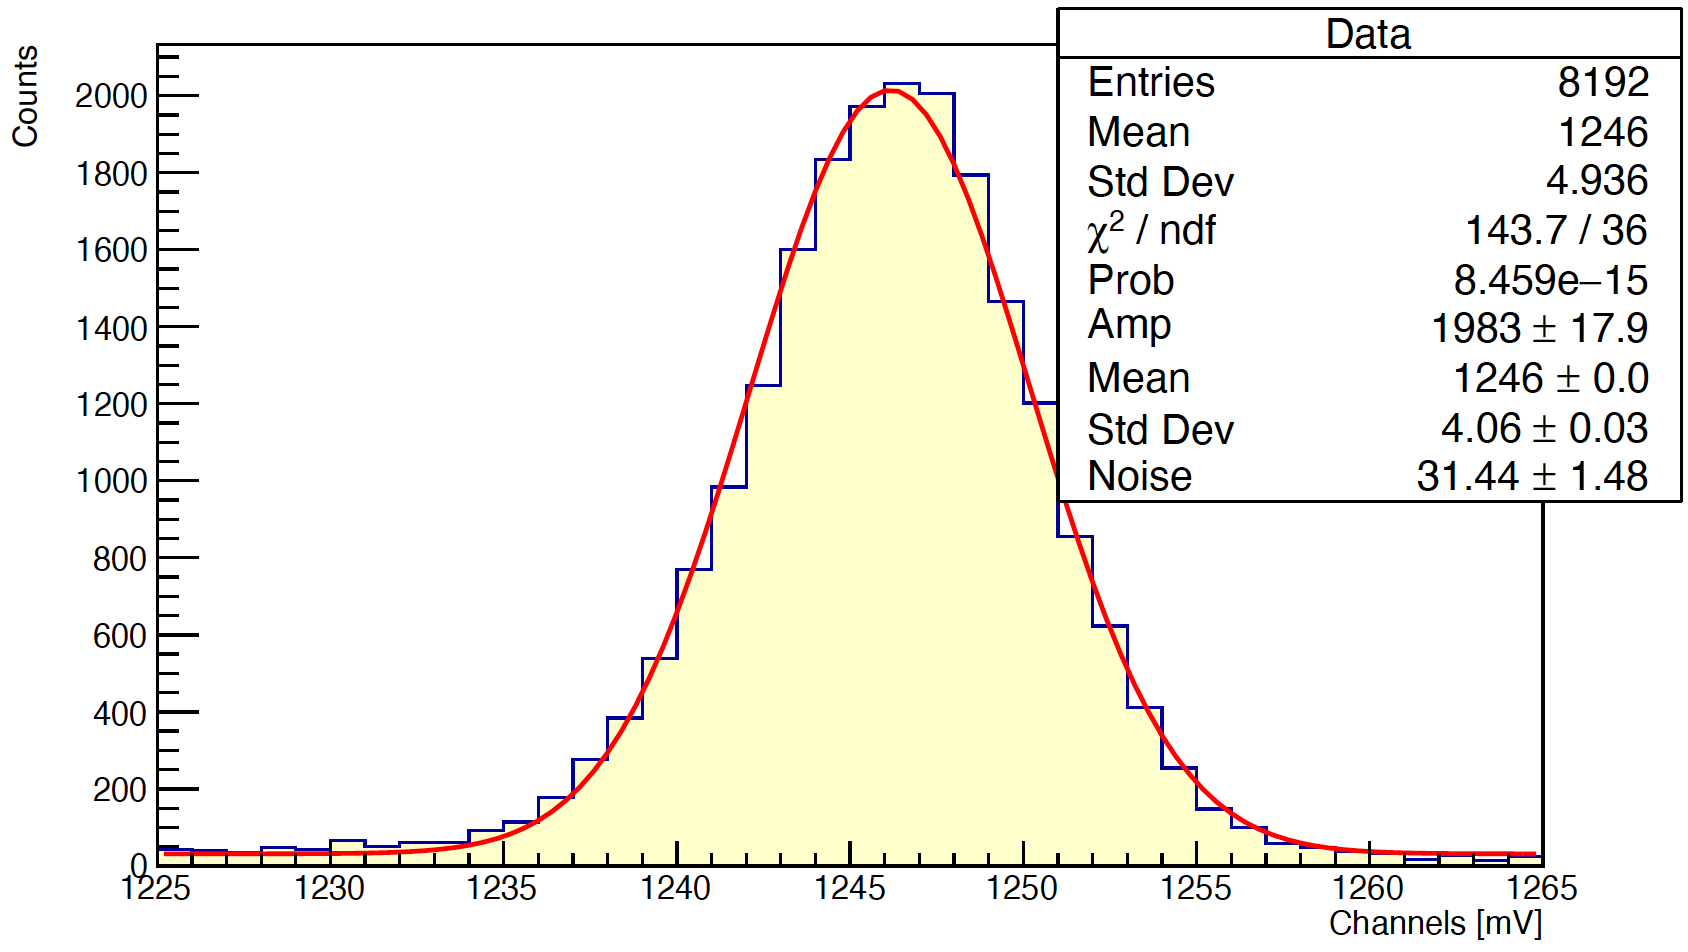
\includegraphics[scale=0.45]{appendice/spettri/NaA1_4}
    \caption{Picco a 511 keV}
\end{figure}
\begin{figure}[H]
    \centering
    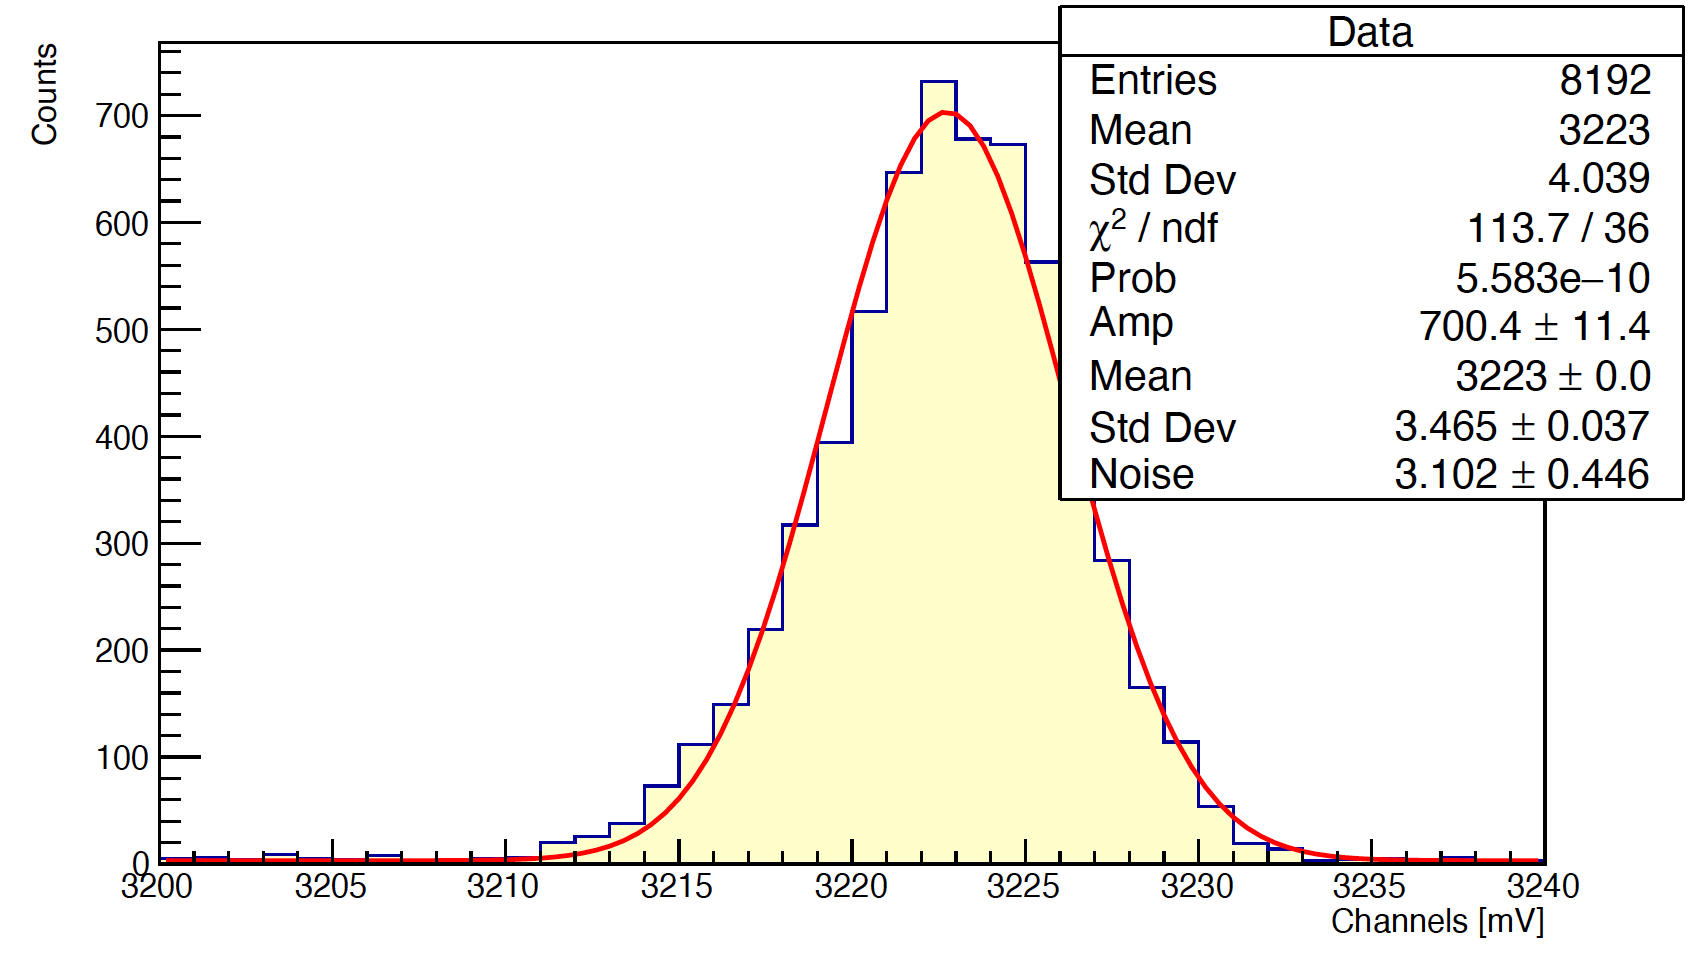
\includegraphics[scale=0.45]{appendice/spettri/NaA2_4}
    \caption{Picco a 1274 keV}
\end{figure}
\begin{figure}[H]
    \centering
    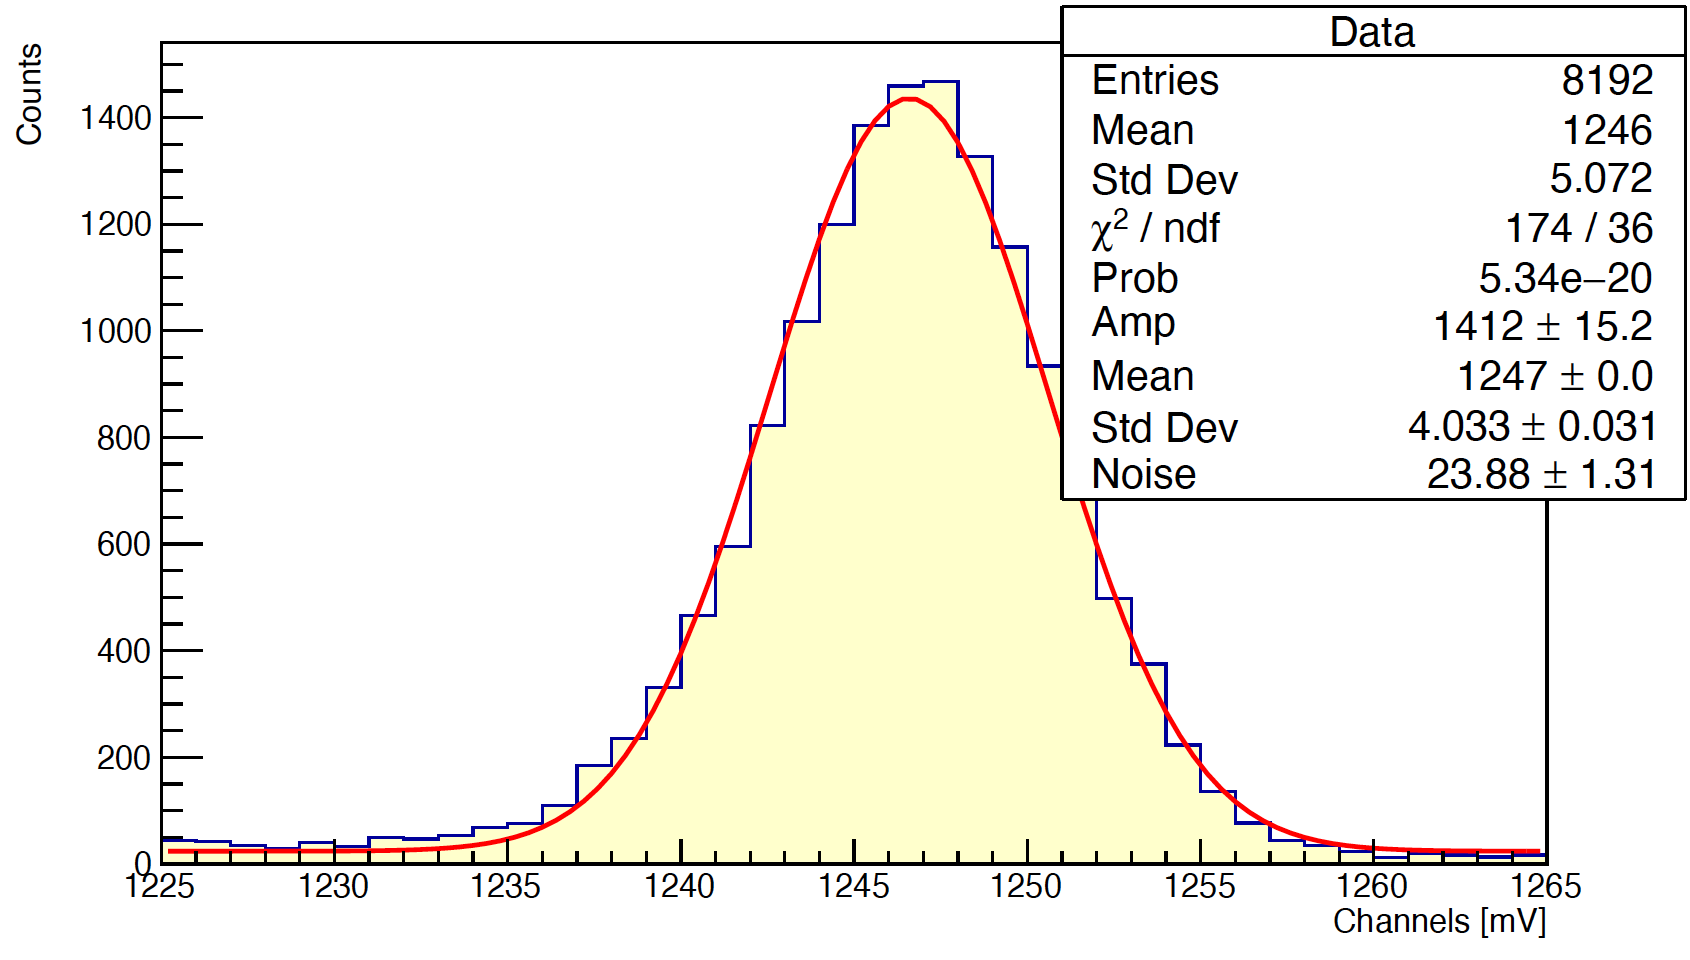
\includegraphics[scale=0.45]{appendice/spettri/NaA1_8}
    \caption{Picco a 511 keV}
\end{figure}
\begin{figure}[H]
    \centering
    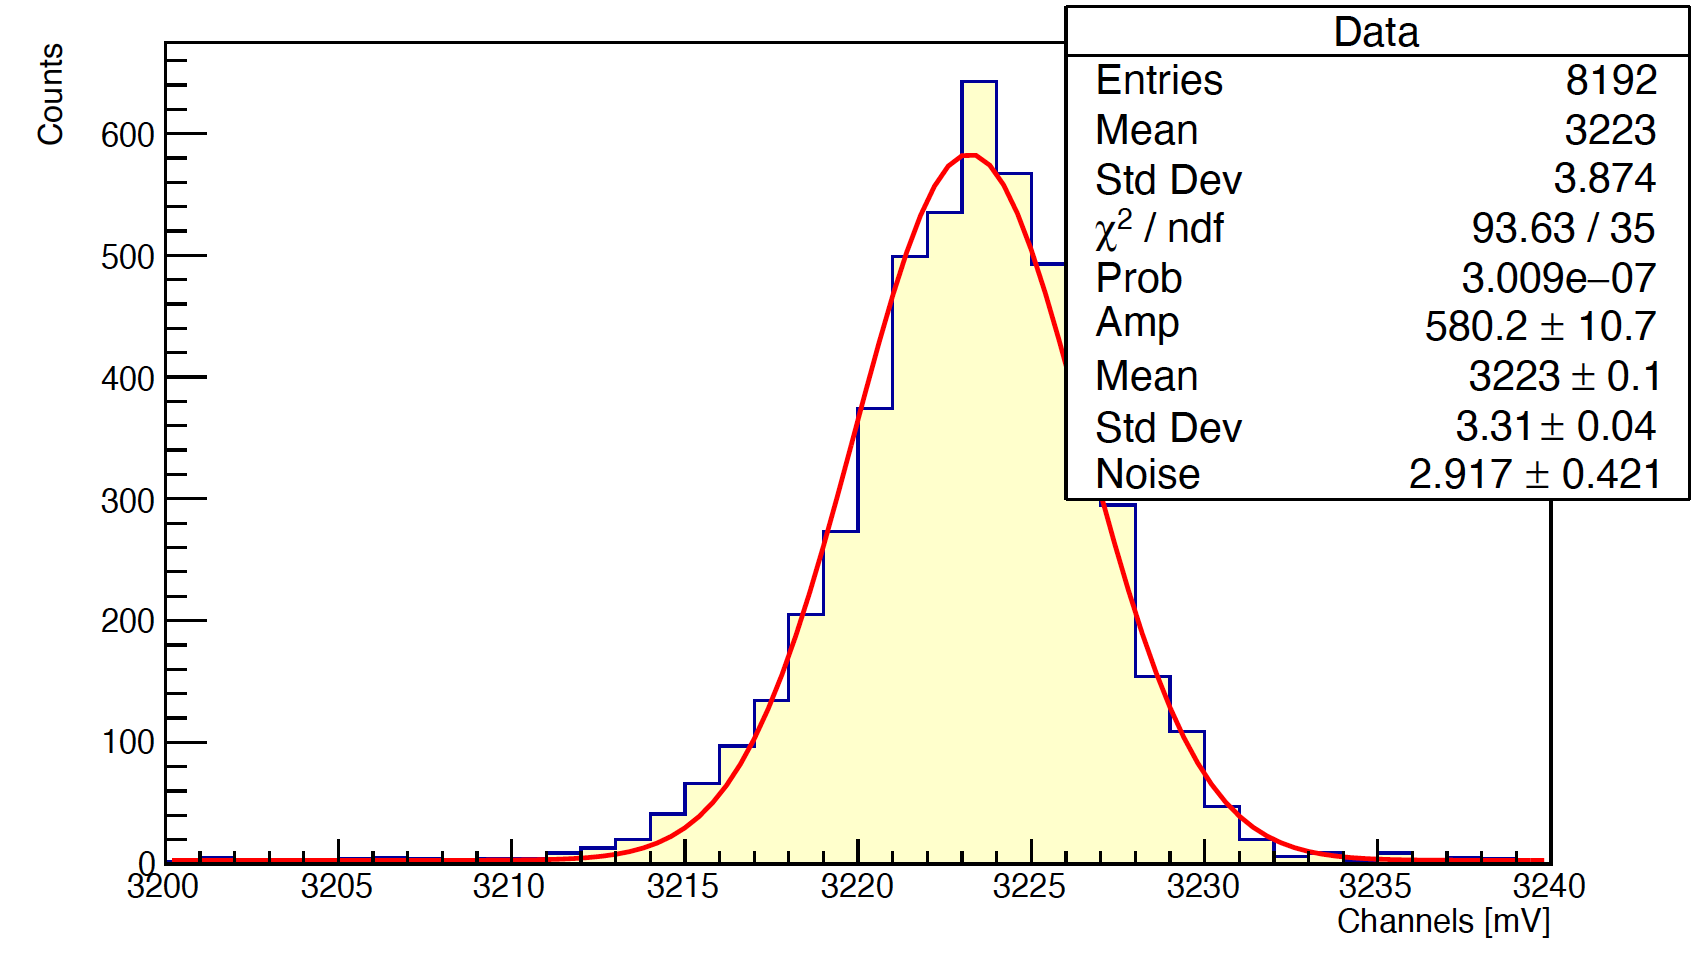
\includegraphics[scale=0.45]{appendice/spettri/NaA2_8}
    \caption{Picco a 1274 keV}
\end{figure}
\begin{figure}[H]
    \centering
    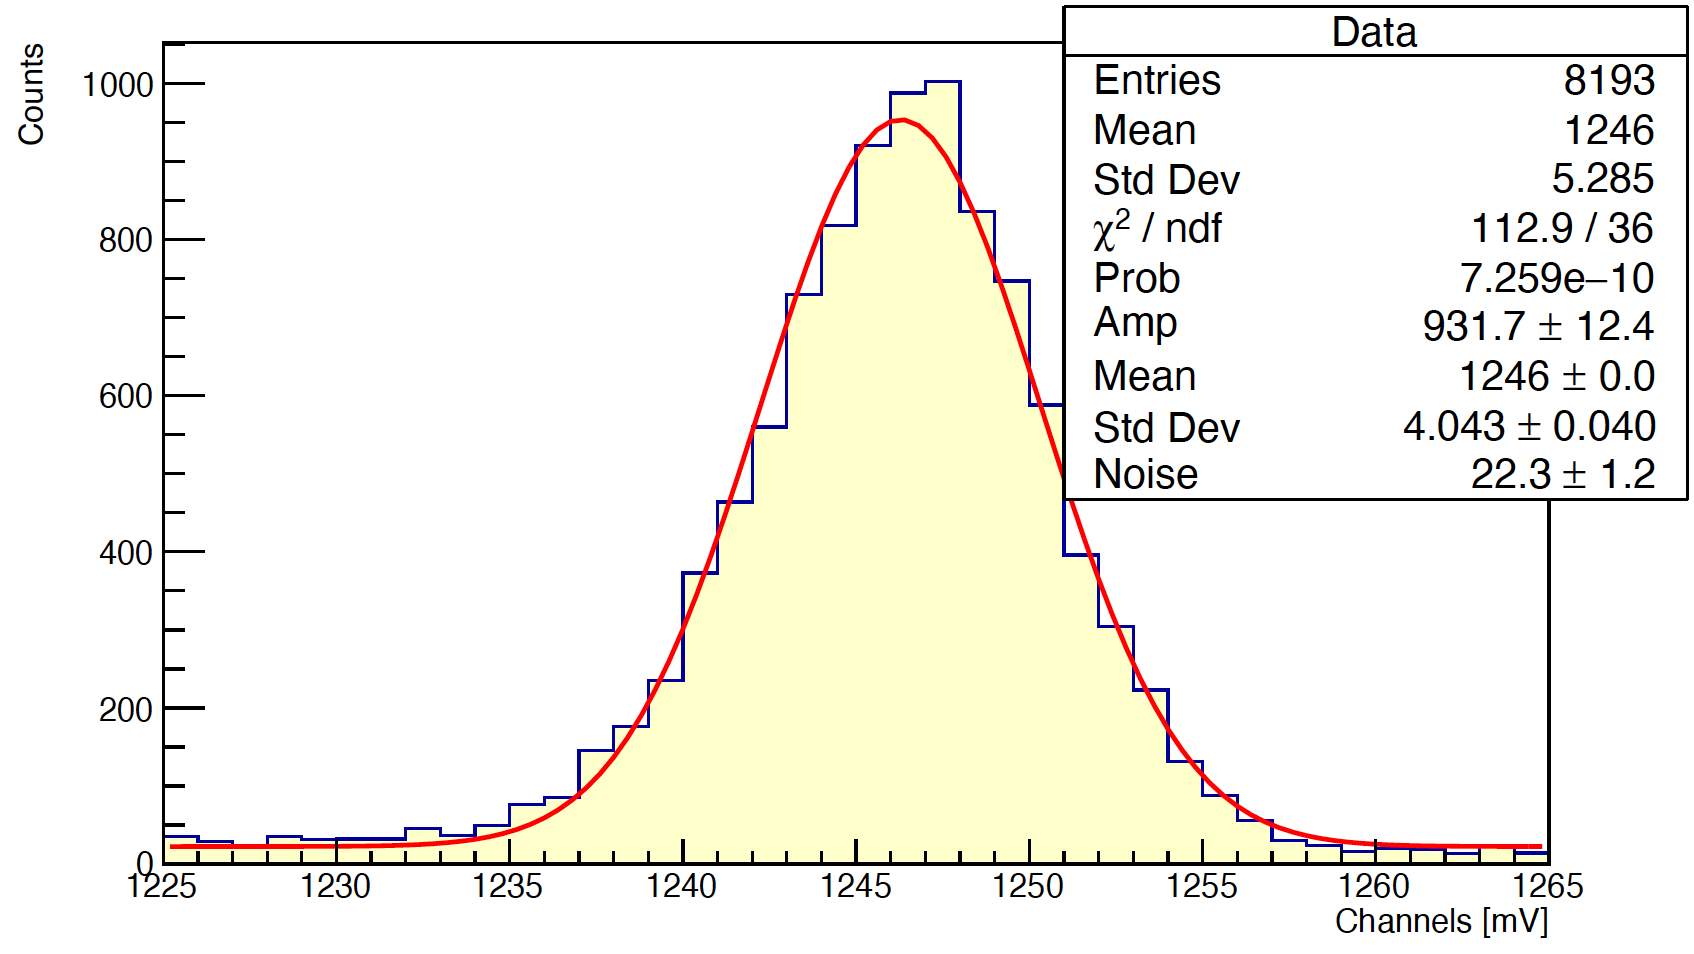
\includegraphics[scale=0.45]{appendice/spettri/NaA1_12}
    \caption{Picco a 511 keV}
\end{figure}
\begin{figure}[H]
    \centering
    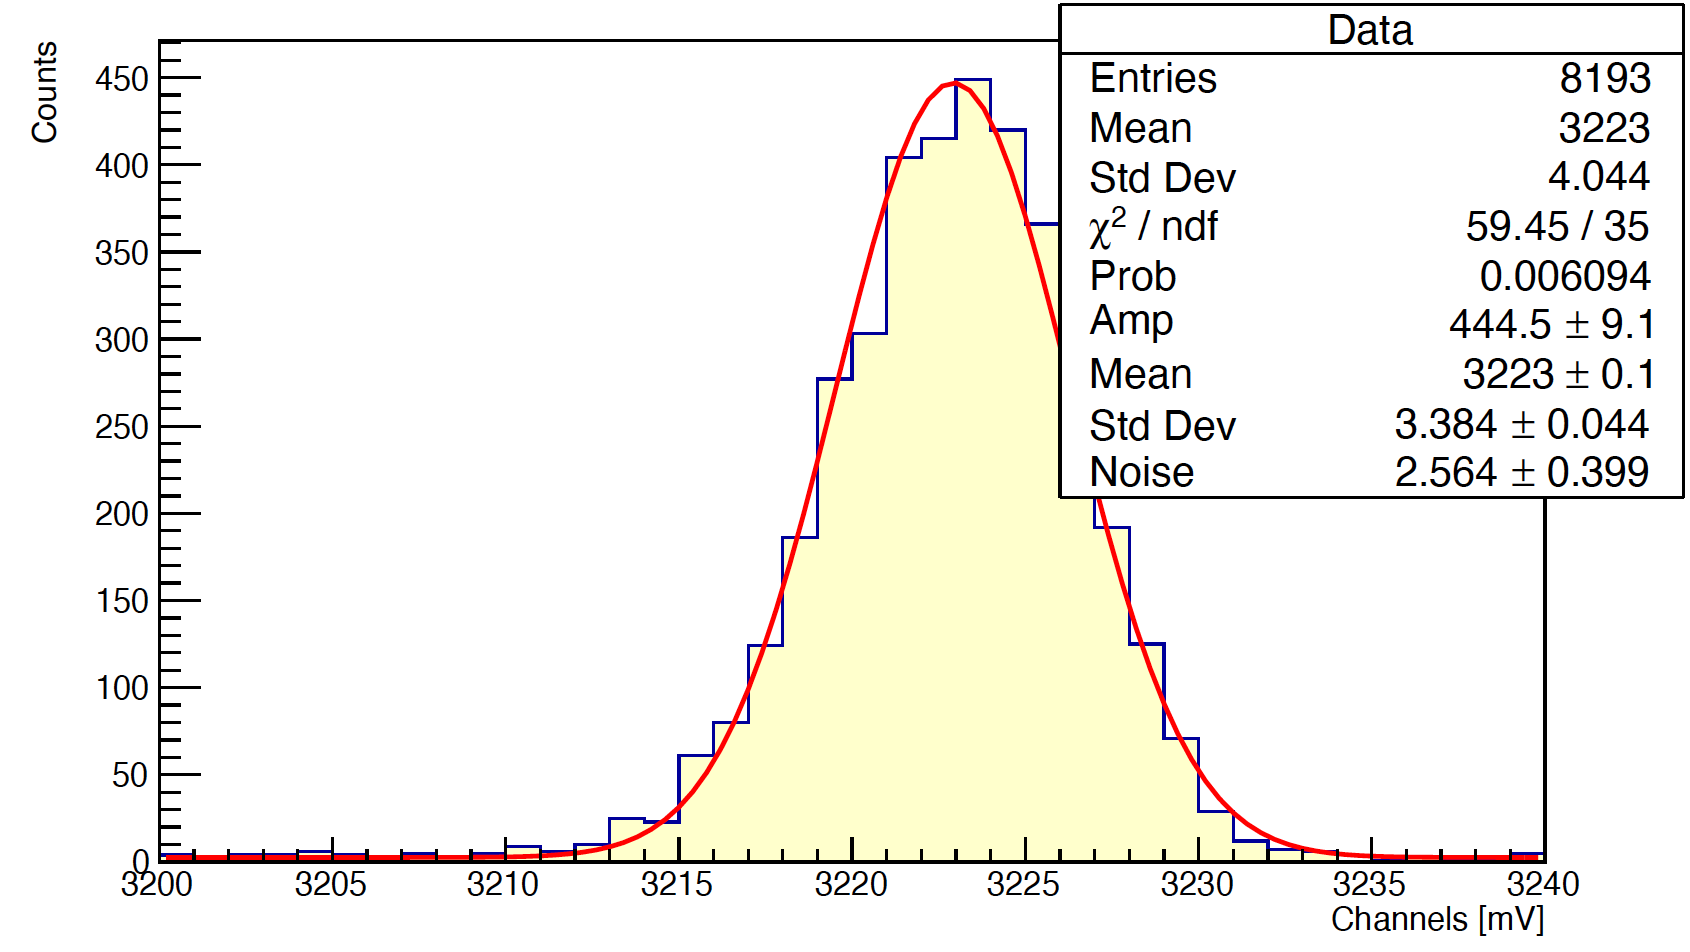
\includegraphics[scale=0.45]{appendice/spettri/NaA2_12}
    \caption{Picco a 1274 keV}
\end{figure}
\begin{figure}[H]
    \centering
    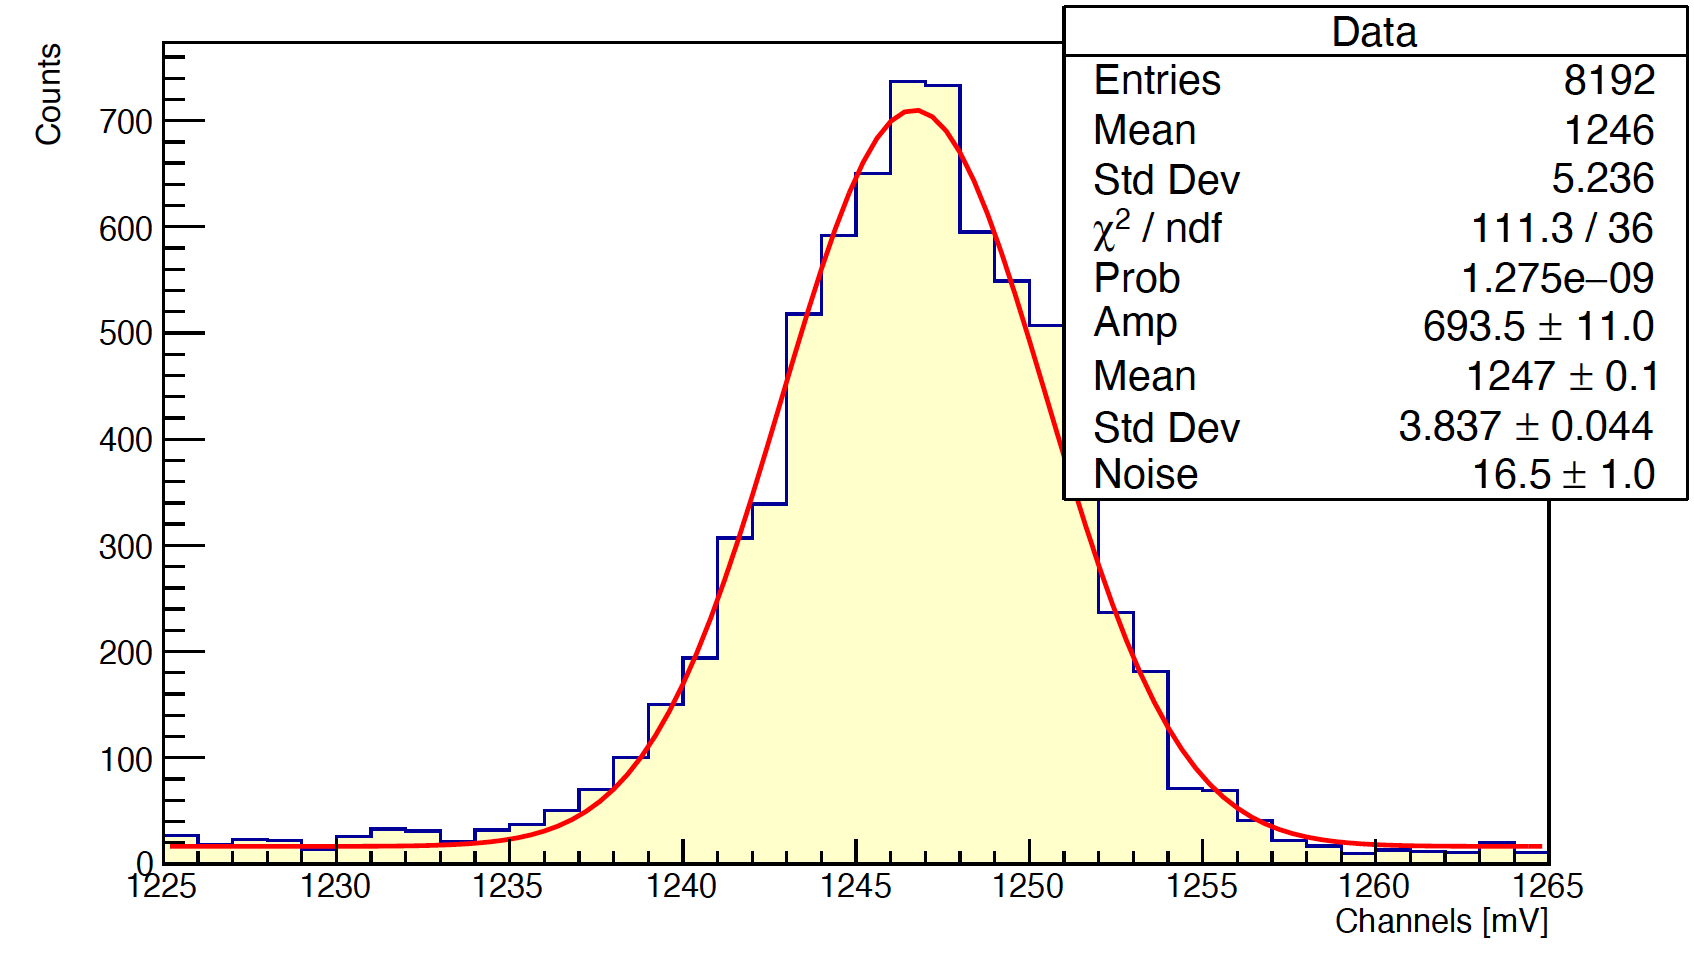
\includegraphics[scale=0.45]{appendice/spettri/NaA1_16}
    \caption{Picco a 511 keV}
\end{figure}
\begin{figure}[H]
    \centering
    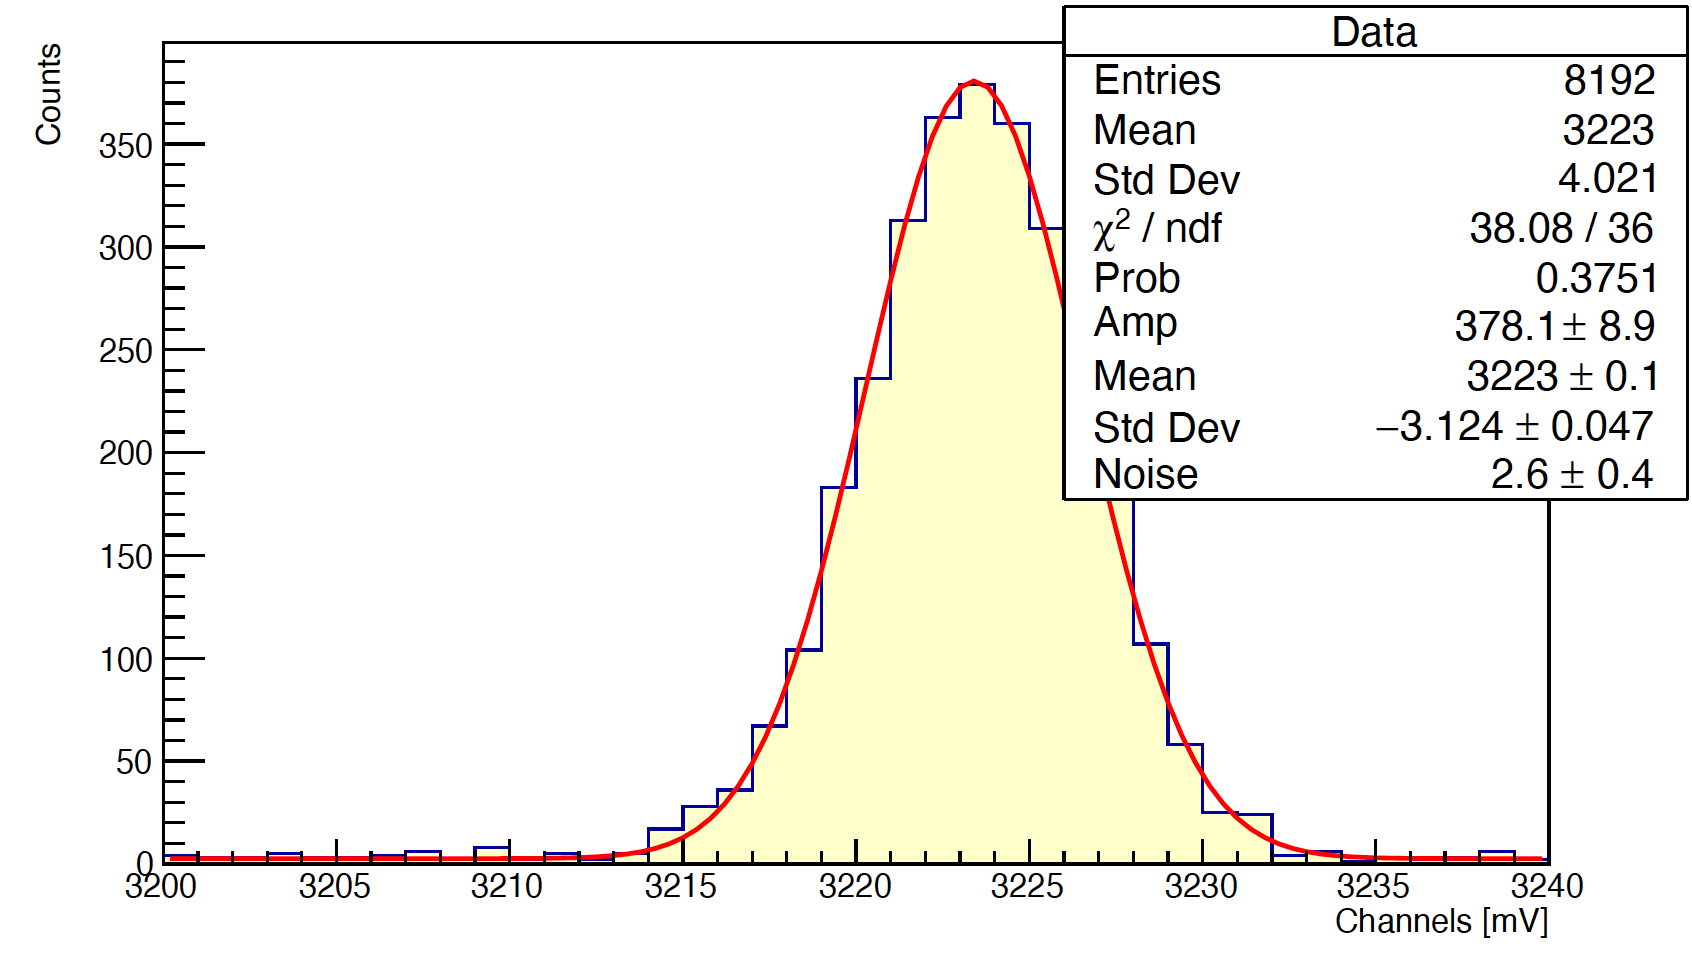
\includegraphics[scale=0.45]{appendice/spettri/NaA2_16}
    \caption{Picco a 1274 keV}
\end{figure}
\begin{figure}[H]
    \centering
    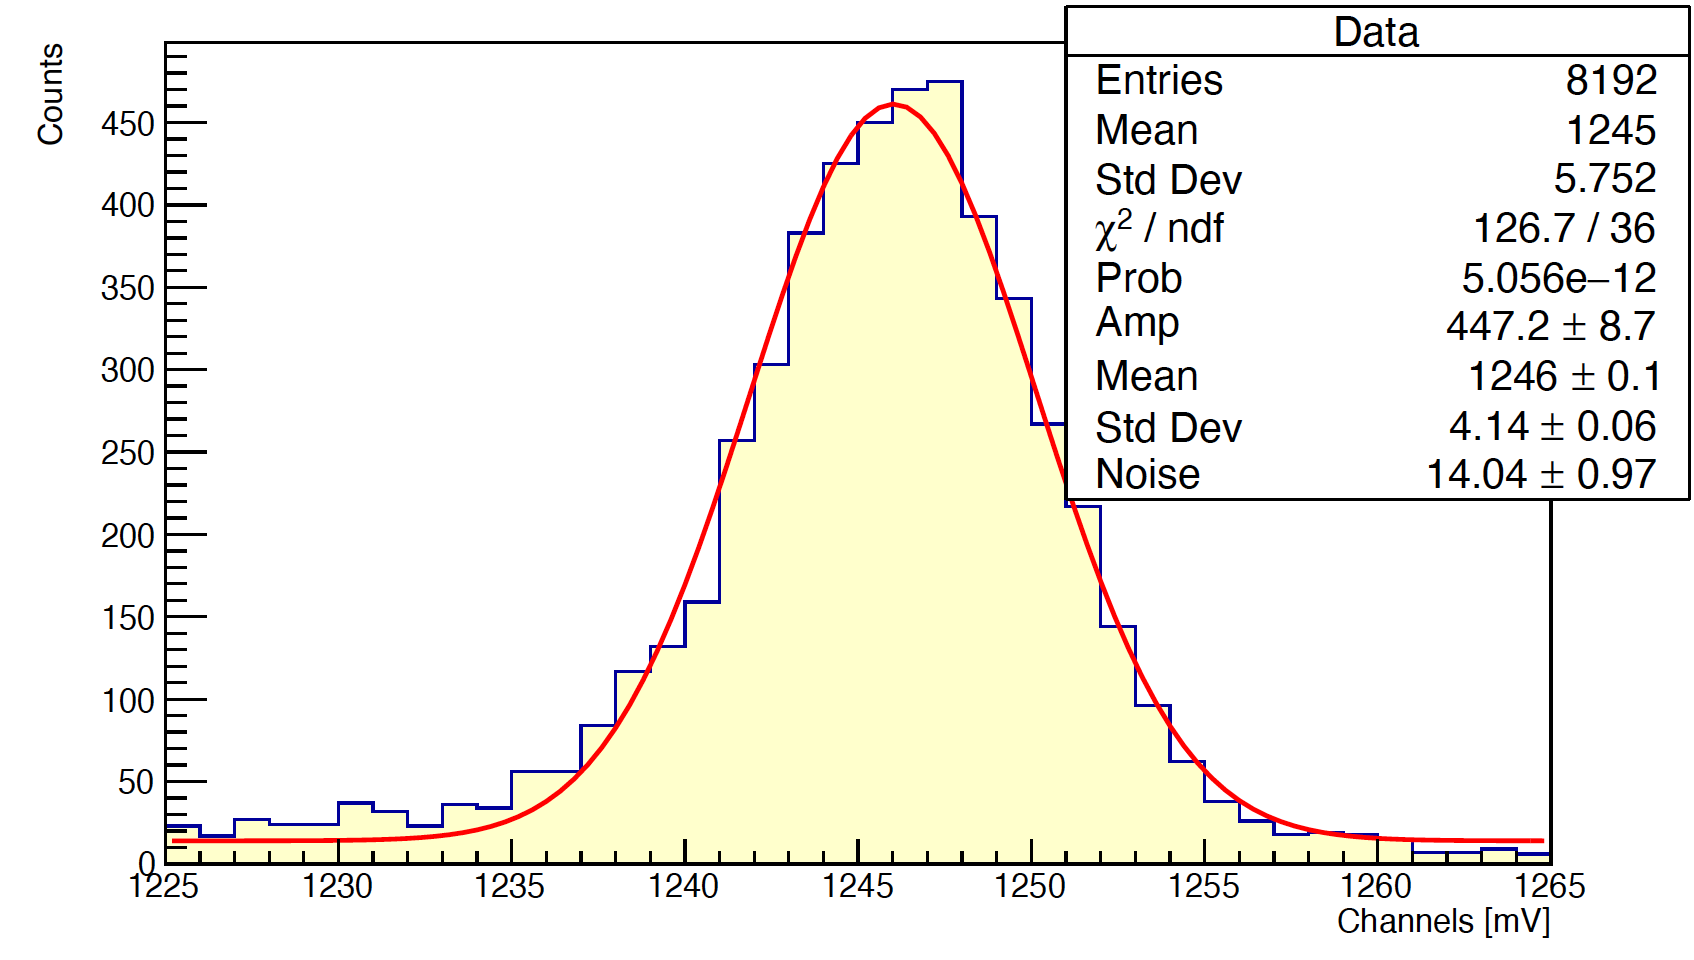
\includegraphics[scale=0.45]{appendice/spettri/NaA1_20}
    \caption{Picco a 511 keV}
\end{figure}
\begin{figure}[H]
    \centering
    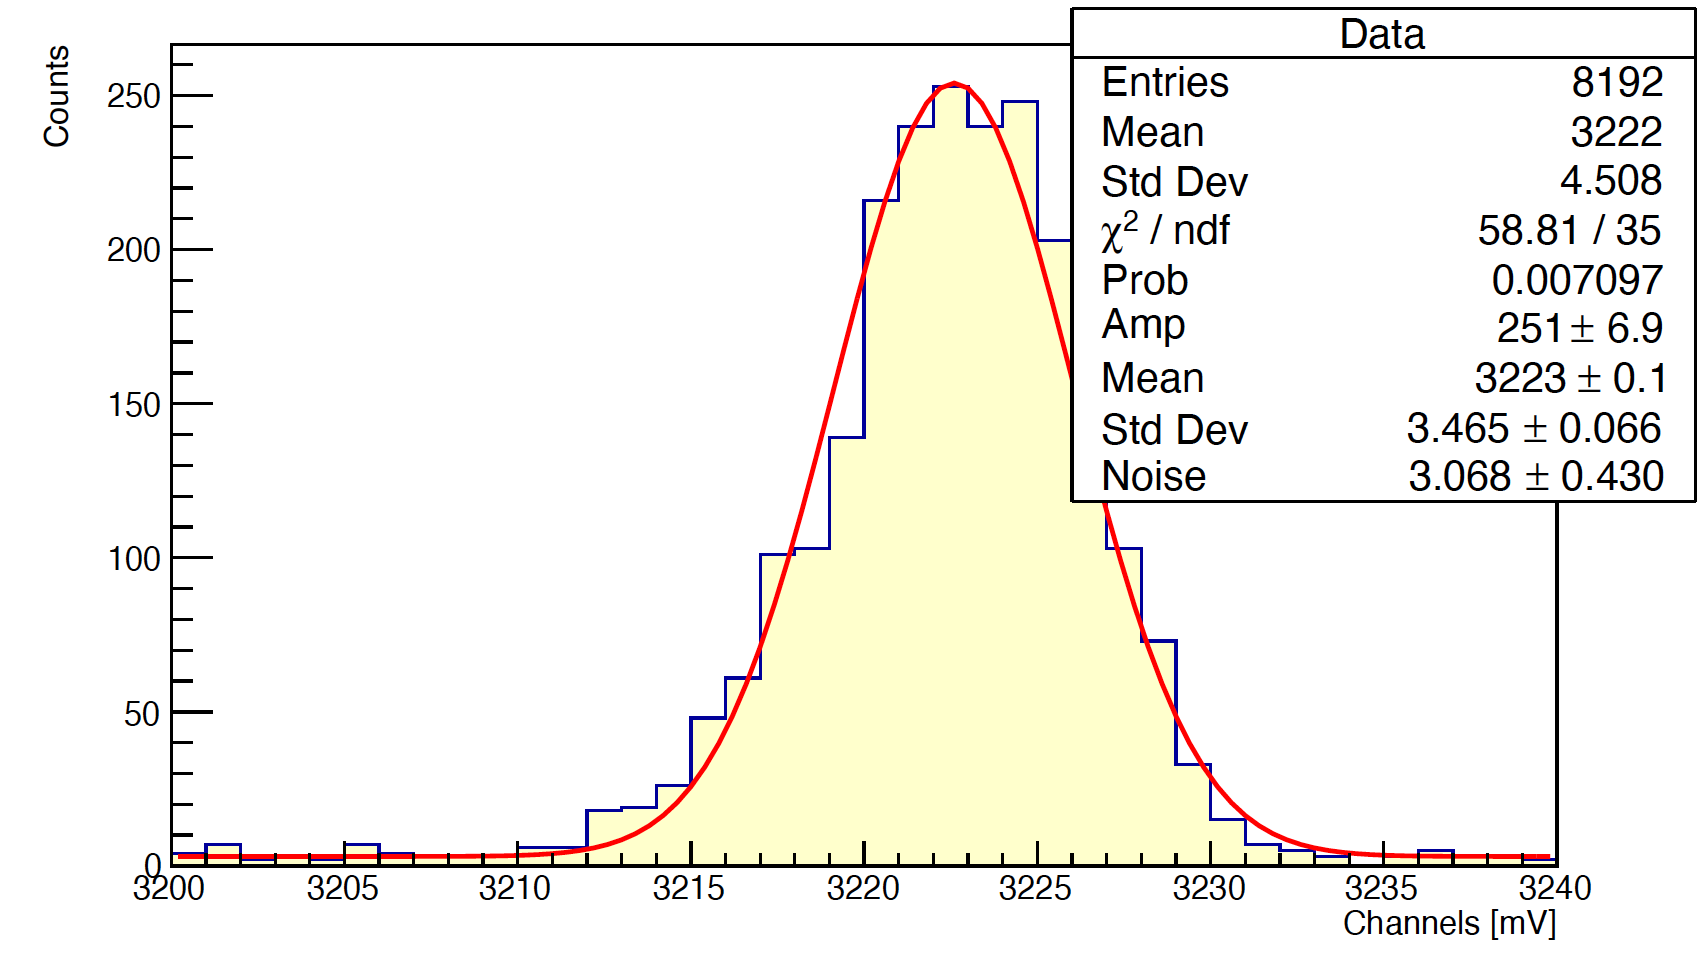
\includegraphics[scale=0.45]{appendice/spettri/NaA2_20}
    \caption{Picco a 1274 keV}
\end{figure}

\subsection{Sodio con rame a 11, 22, 33, 44 e 54 cm di spessore}
\begin{figure}[H]
    \centering
    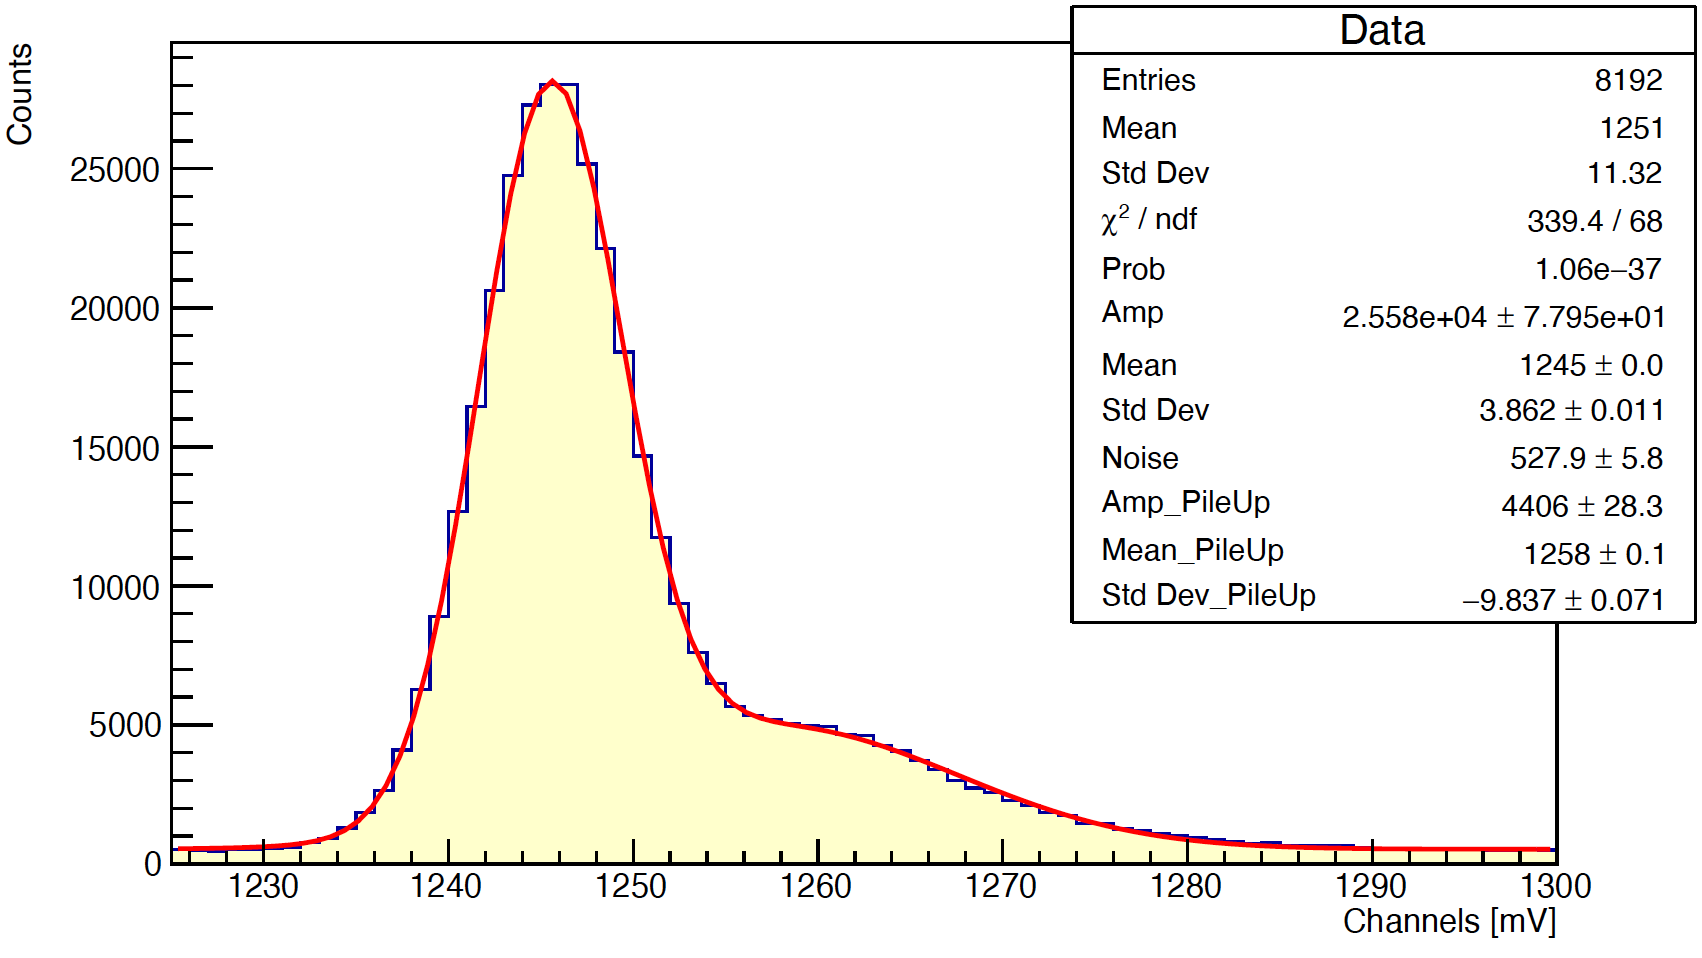
\includegraphics[scale=0.45]{appendice/spettri/NaCu1_11}
    \caption{Picco a 511 keV}
\end{figure}
\begin{figure}[H]
    \centering
    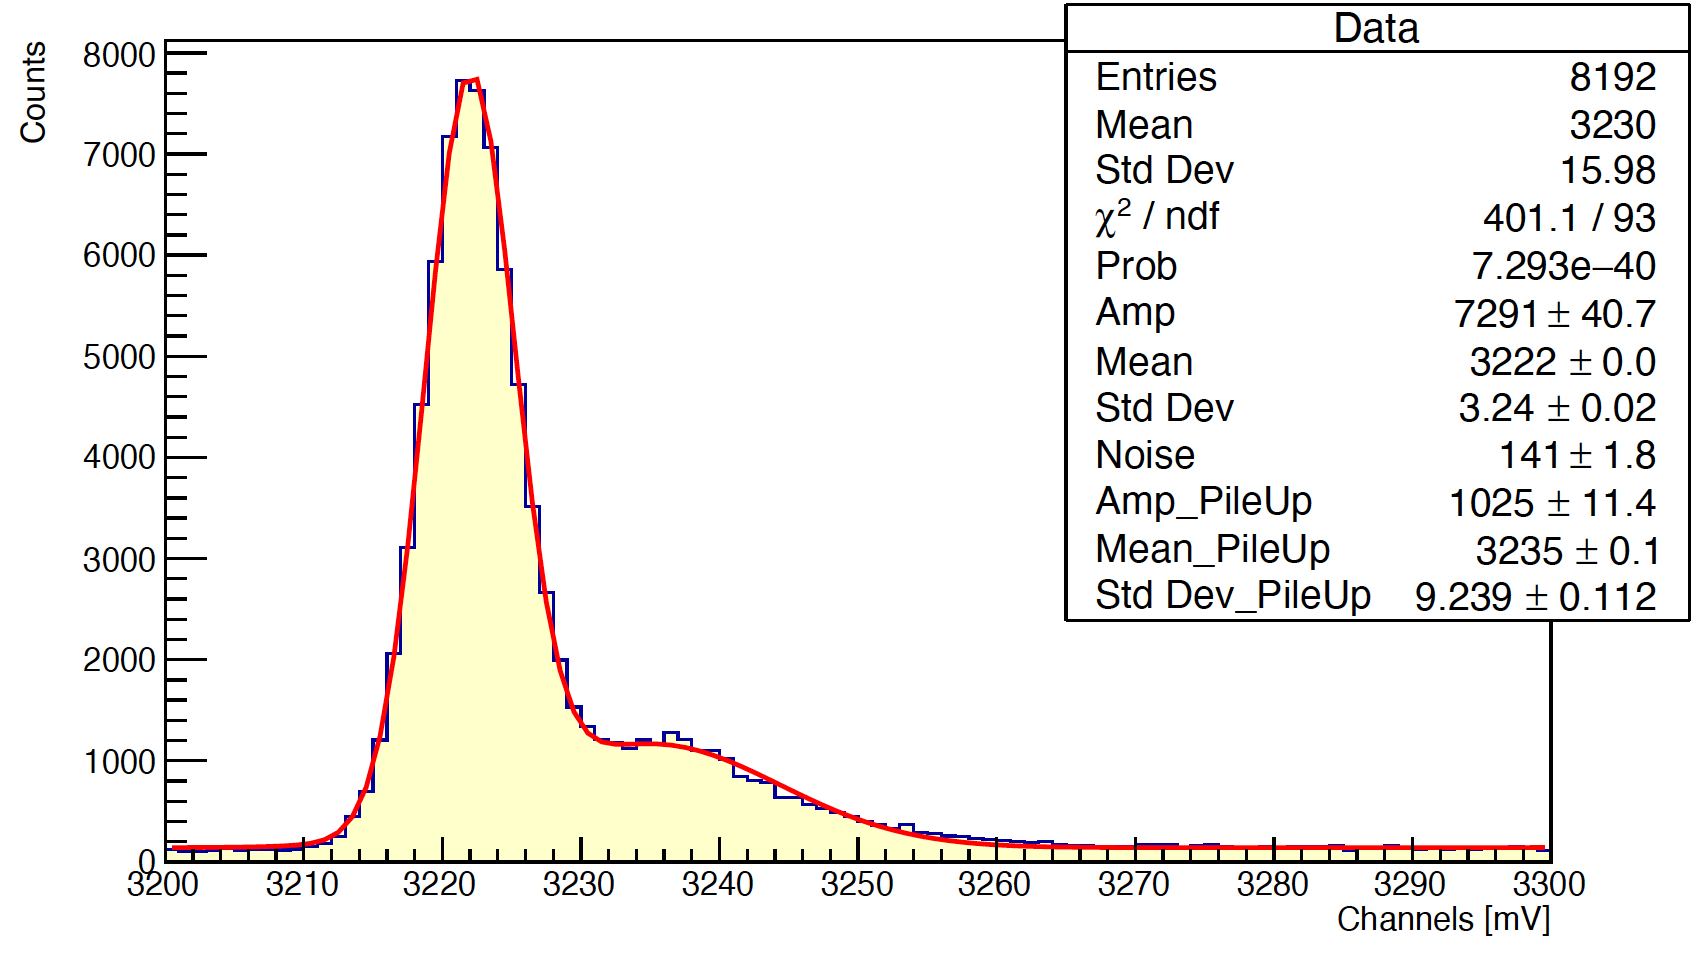
\includegraphics[scale=0.45]{appendice/spettri/NaCu2_11}
    \caption{Picco a 1274 keV}
\end{figure}
\begin{figure}[H]
    \centering
    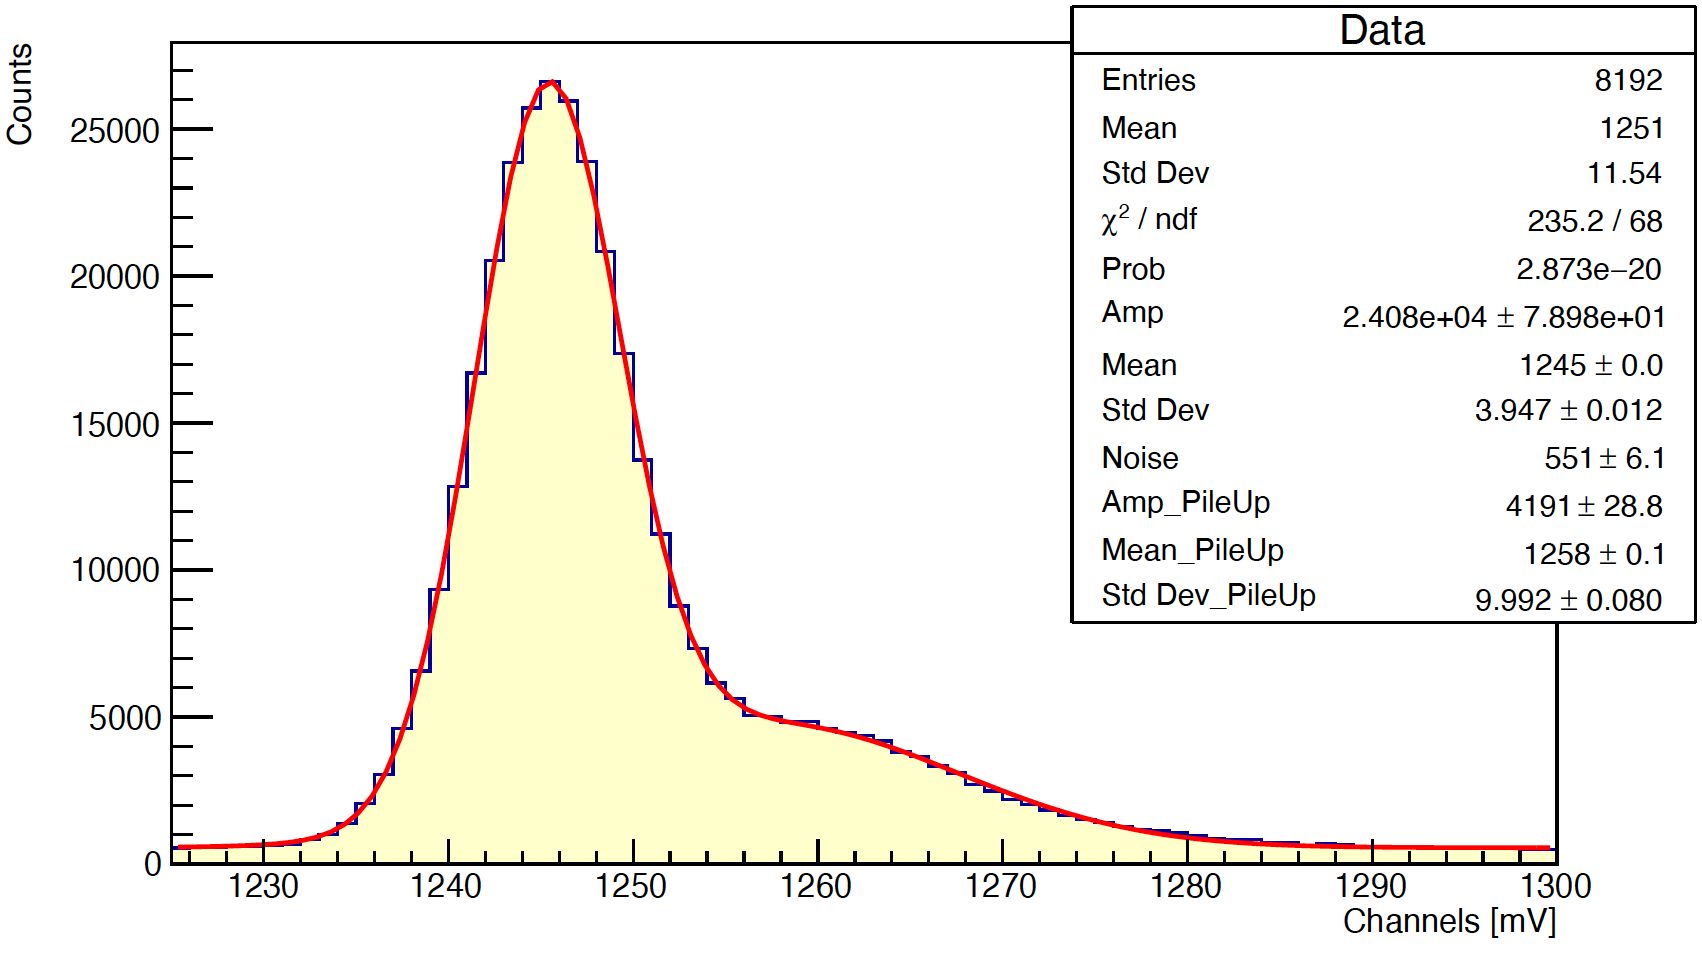
\includegraphics[scale=0.45]{appendice/spettri/NaCu1_22}
    \caption{Picco a 511 keV}
\end{figure}
\begin{figure}[H]
    \centering
    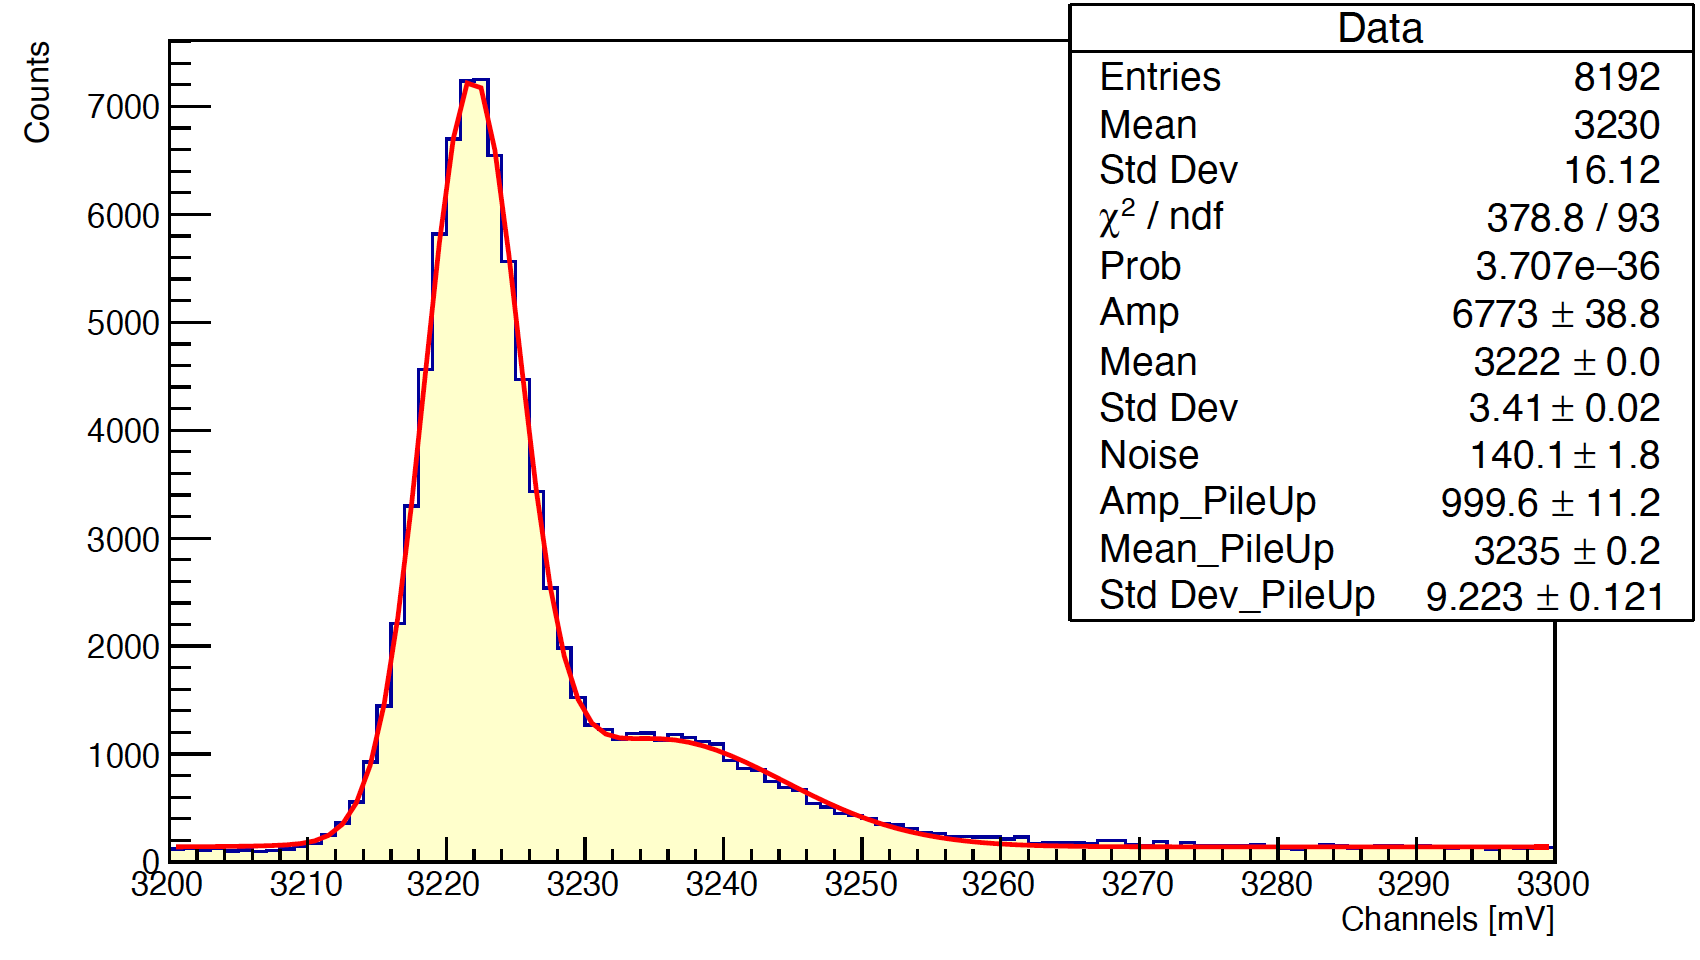
\includegraphics[scale=0.45]{appendice/spettri/NaCu2_22}
    \caption{Picco a 1274 keV}
\end{figure}
\begin{figure}[H]
    \centering
    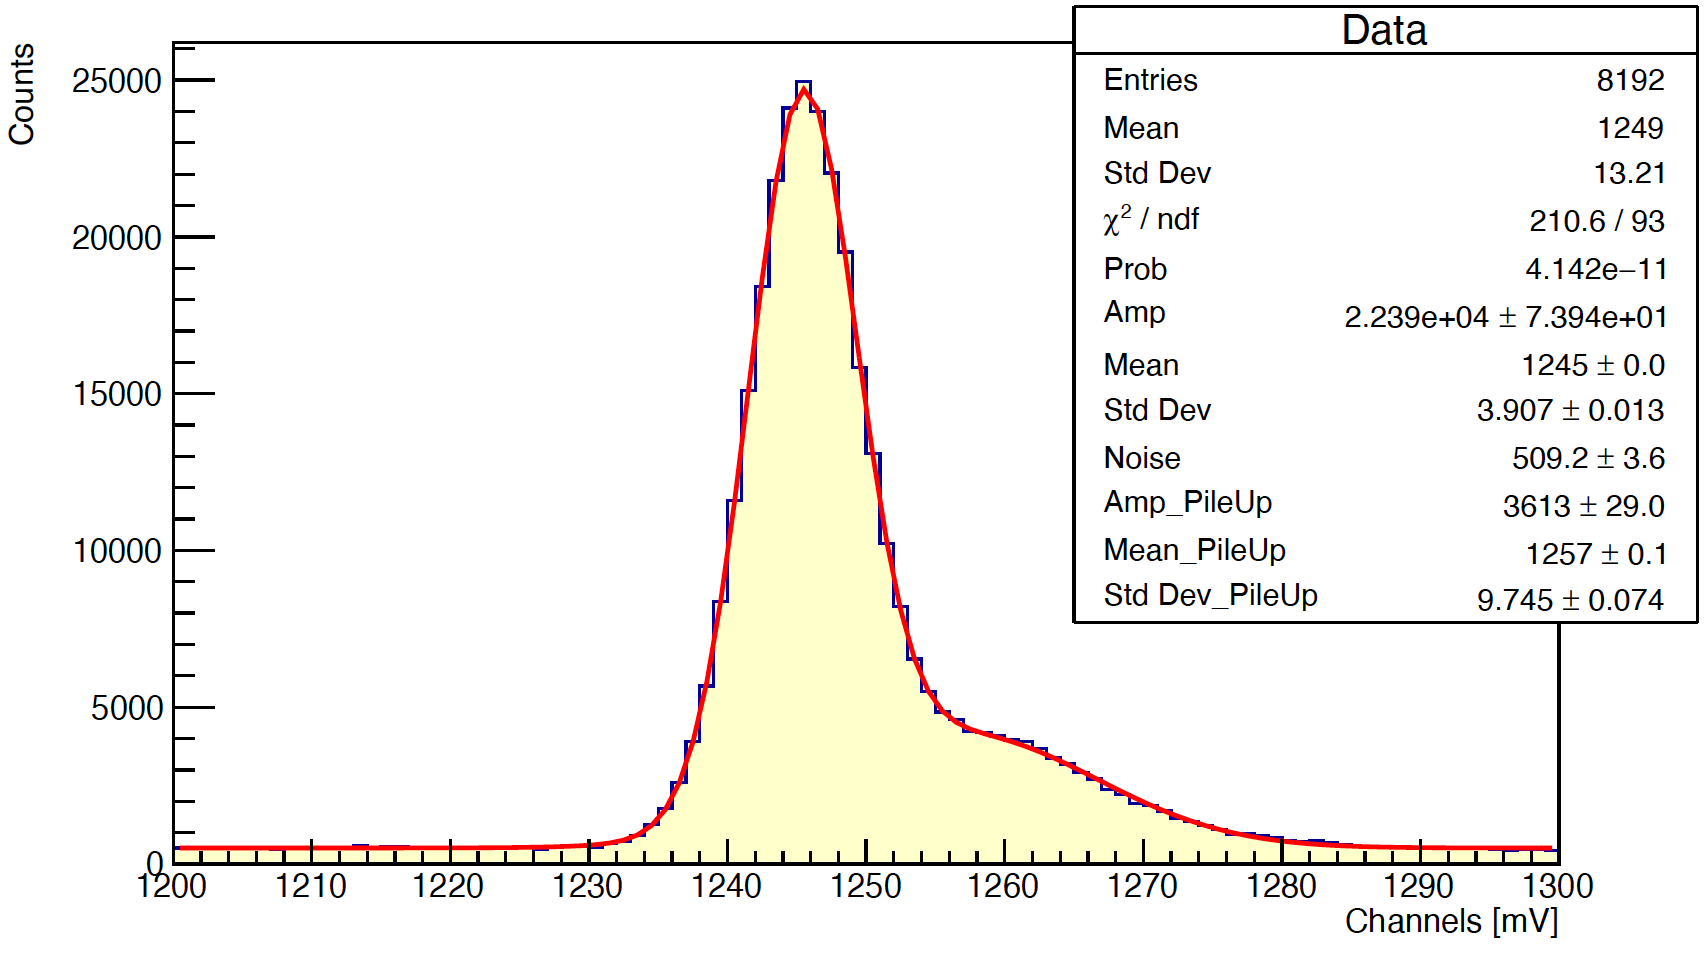
\includegraphics[scale=0.45]{appendice/spettri/NaCu1_33}
    \caption{Picco a 511 keV}
\end{figure}
\begin{figure}[H]
    \centering
    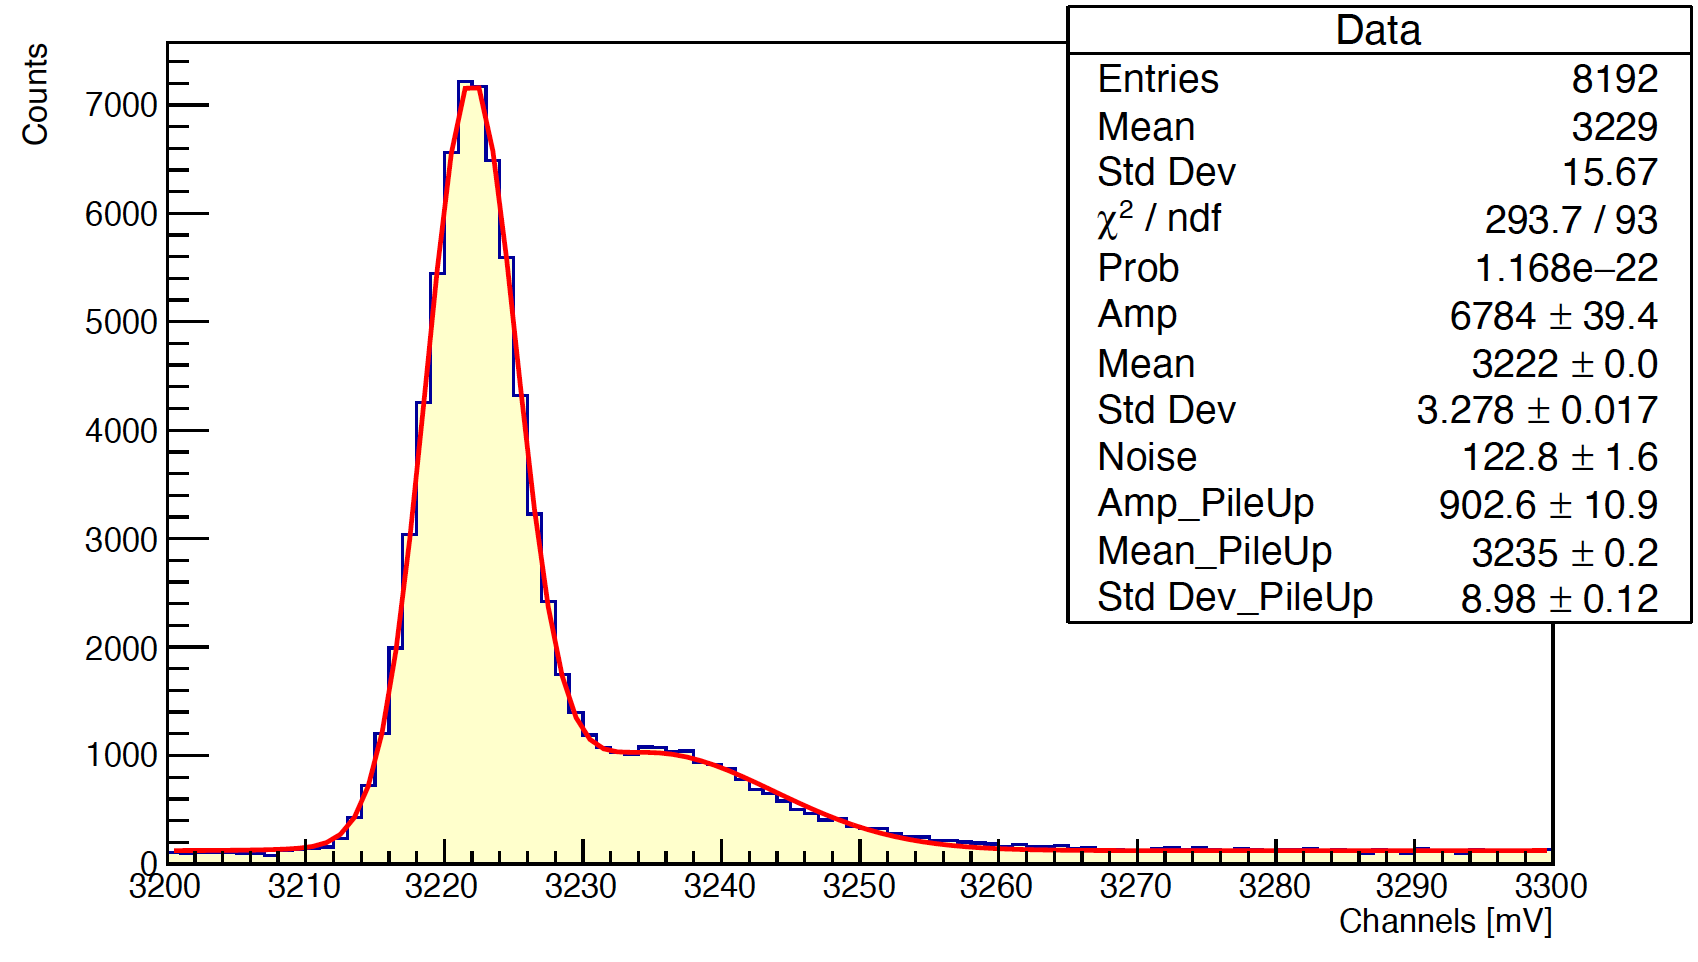
\includegraphics[scale=0.45]{appendice/spettri/NaCu2_33}
    \caption{Picco a 1274 keV}
\end{figure}
\begin{figure}[H]
    \centering
    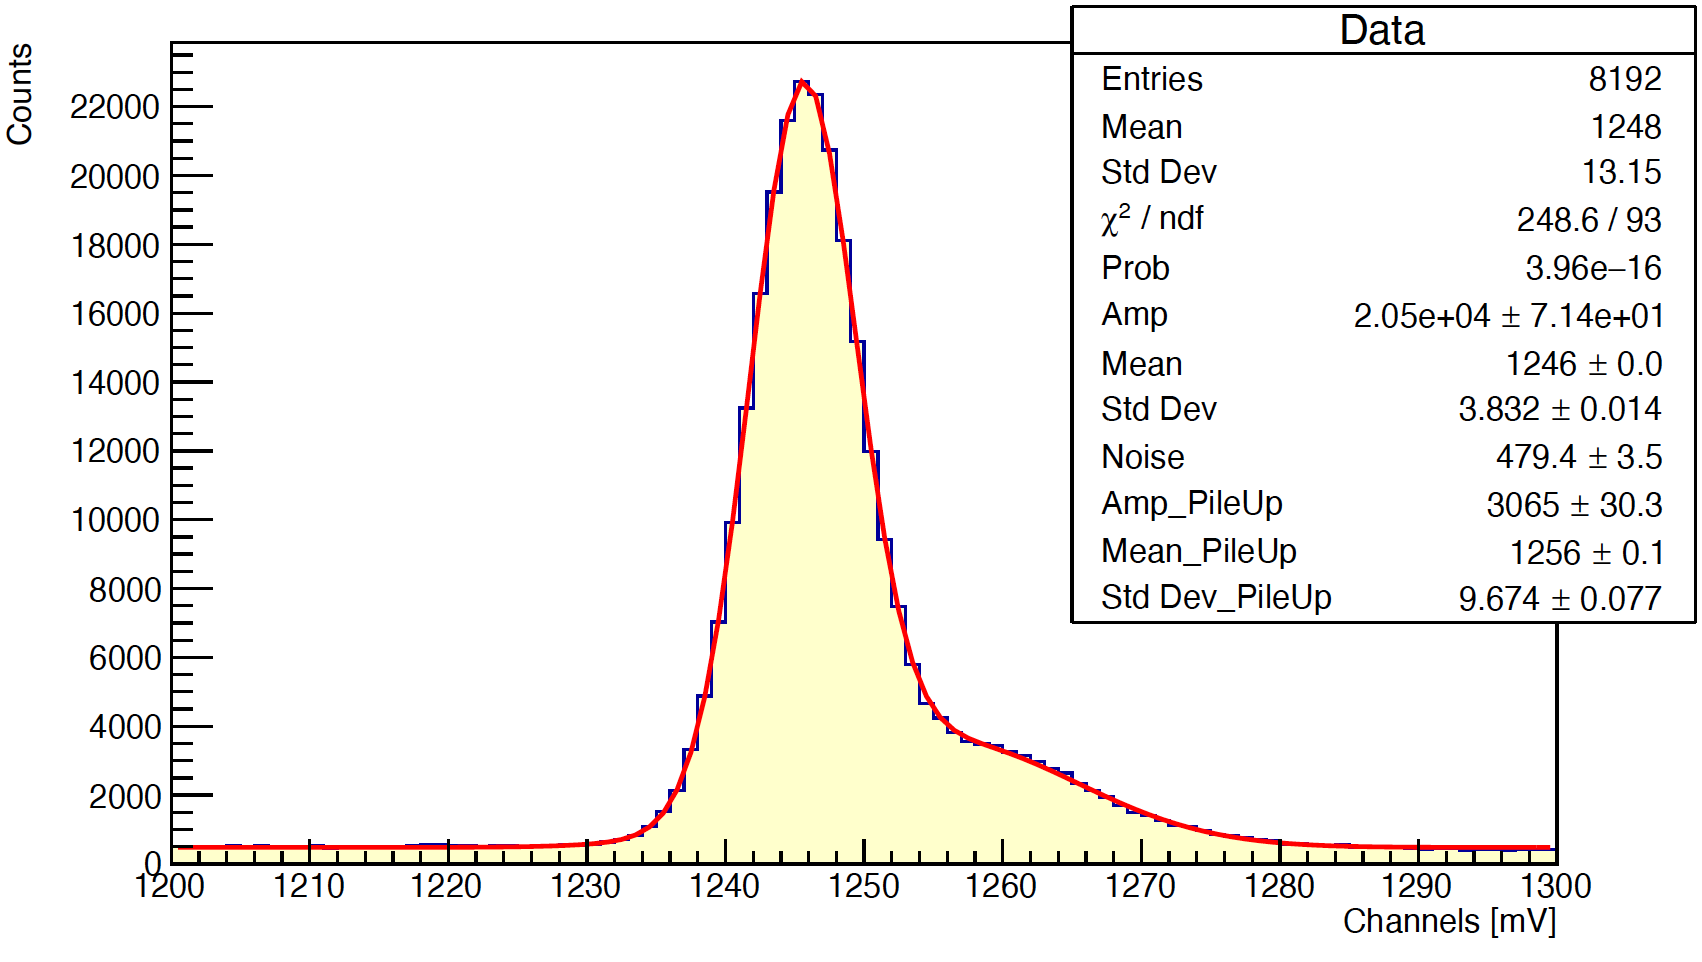
\includegraphics[scale=0.45]{appendice/spettri/NaCu1_44}
    \caption{Picco a 511 keV}
\end{figure}
\begin{figure}[H]
    \centering
    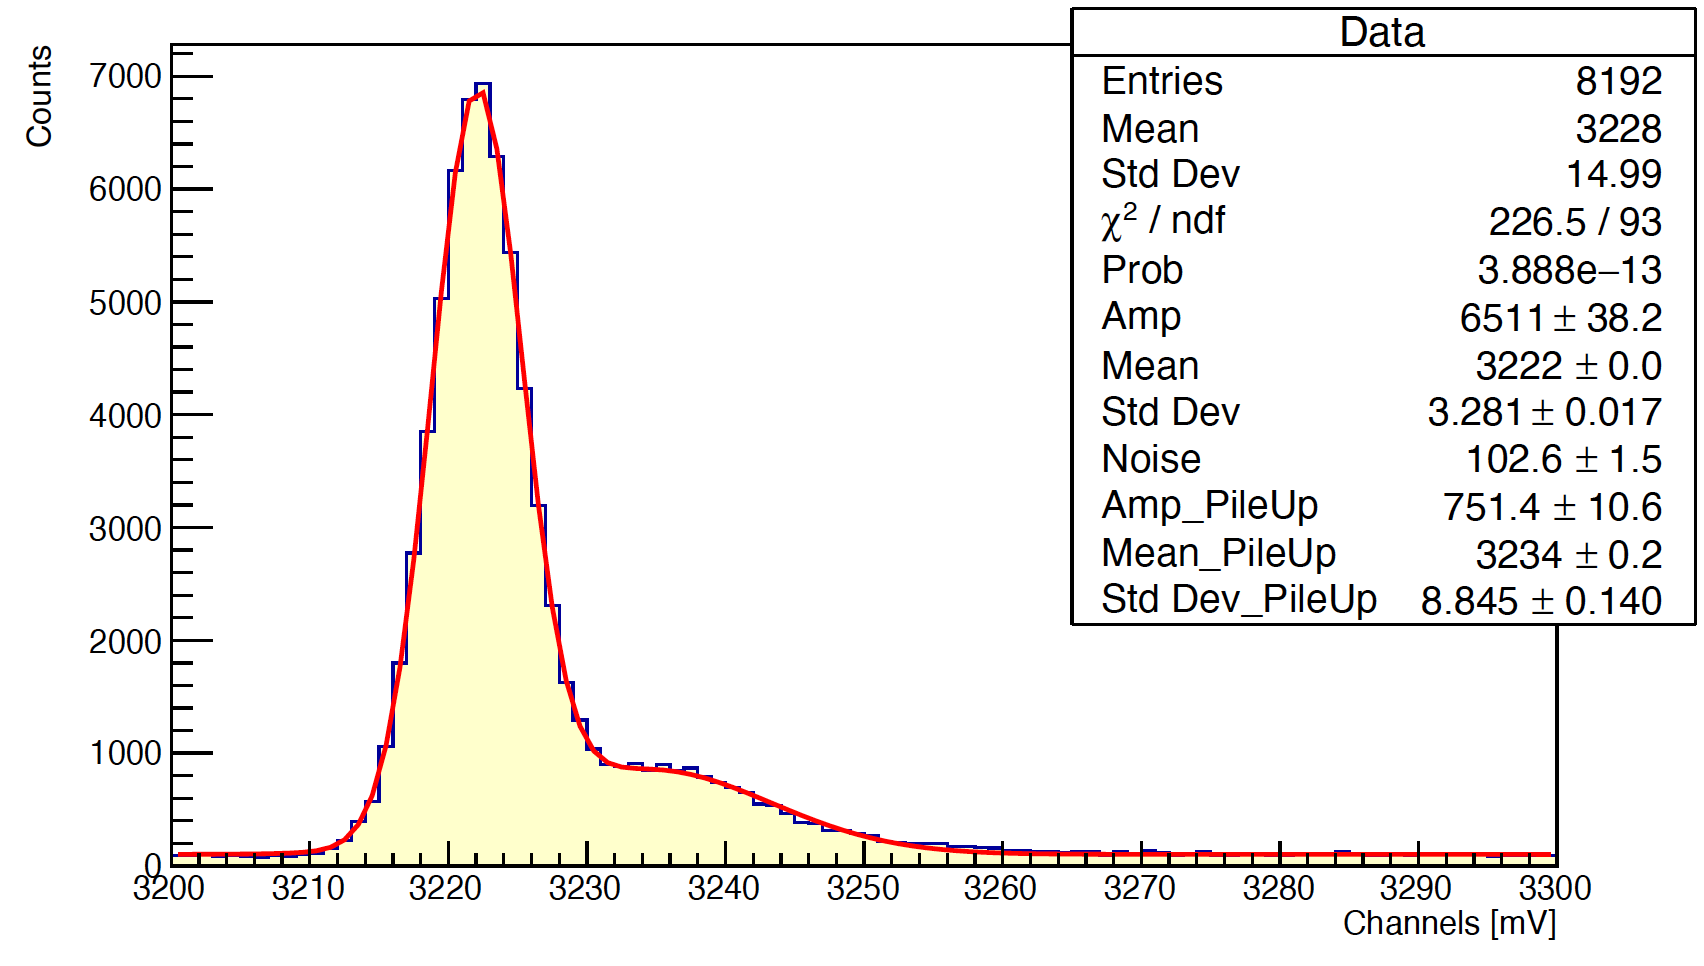
\includegraphics[scale=0.45]{appendice/spettri/NaCu2_44}
    \caption{Picco a 1274 keV}
\end{figure}
\begin{figure}[H]
    \centering
    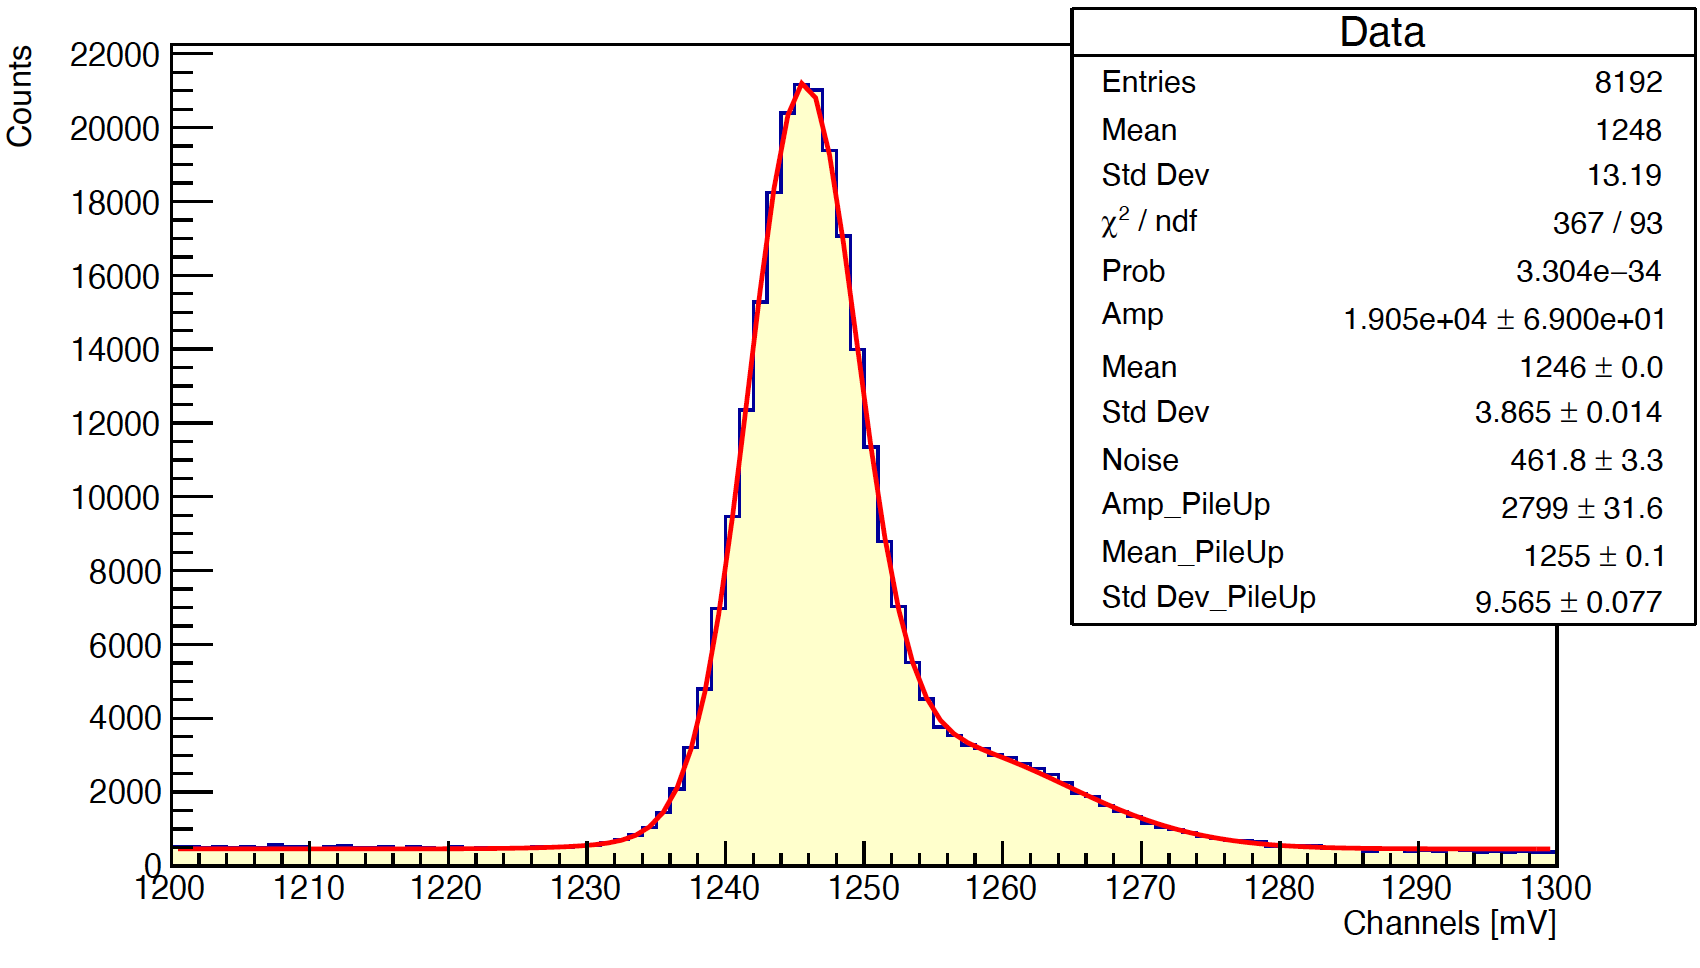
\includegraphics[scale=0.45]{appendice/spettri/NaCu1_54}
    \caption{Picco a 511 keV}
\end{figure}
\begin{figure}[H]
    \centering
    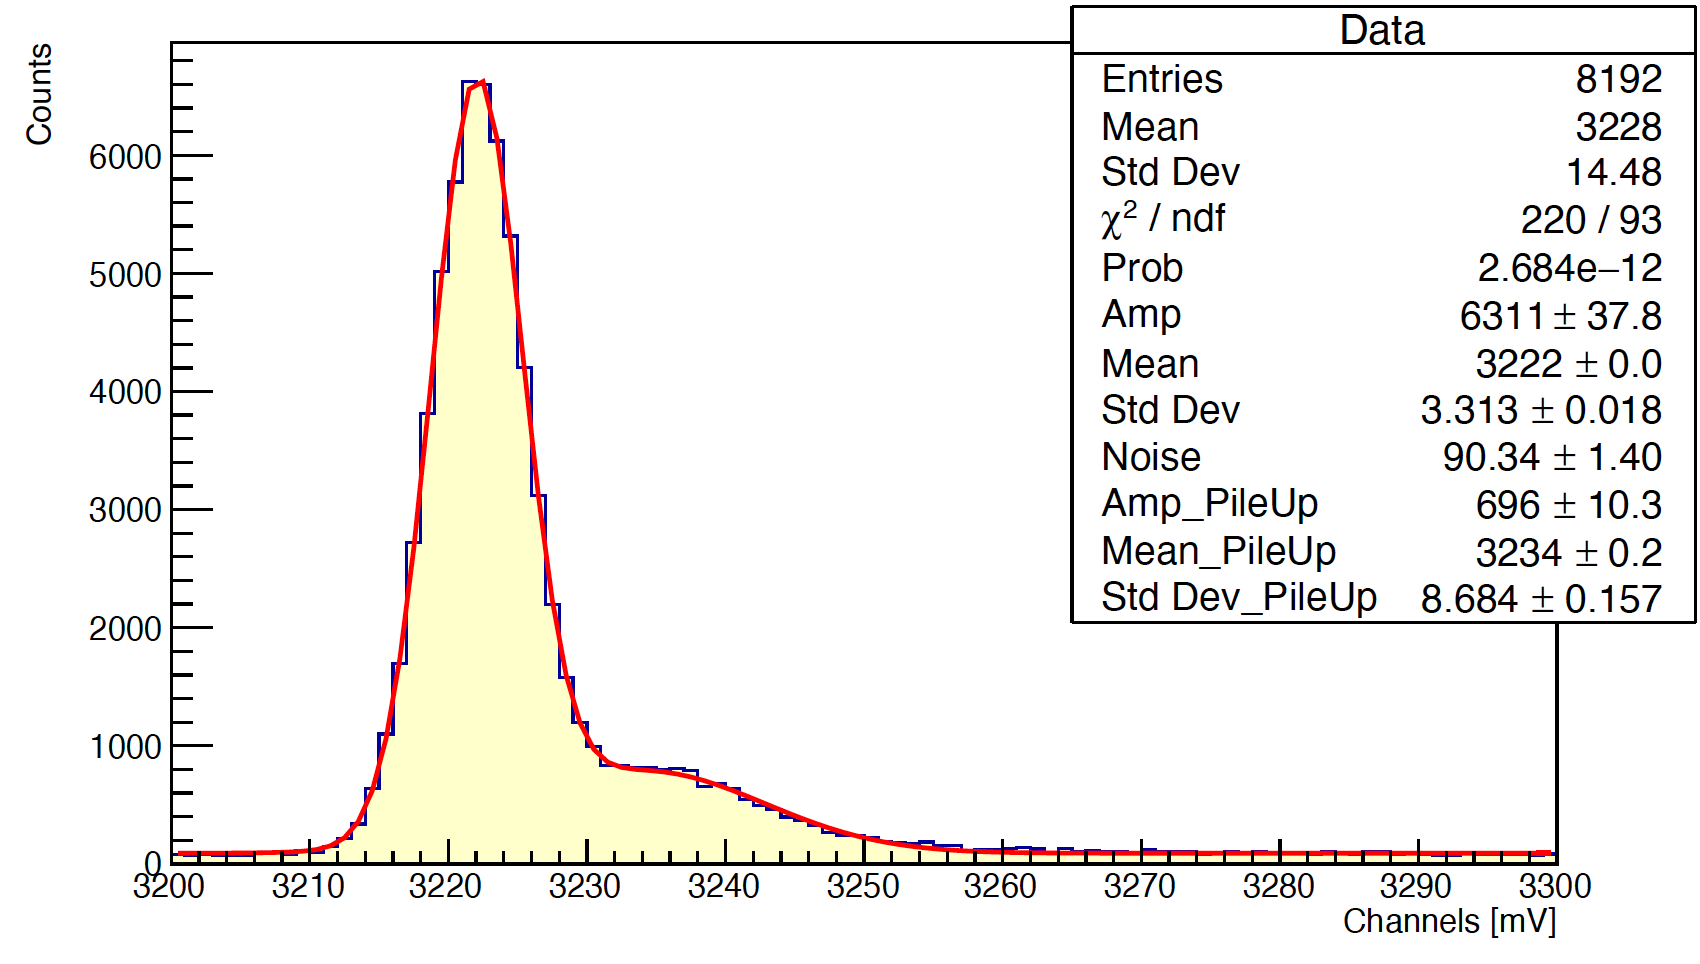
\includegraphics[scale=0.45]{appendice/spettri/NaCu2_54}
    \caption{Picco a 1274 keV}
\end{figure}

\subsection{Sodio con piombo a 1, 21, 33, 58 e 108 cm di spessore}
\begin{figure}[H]
    \centering
    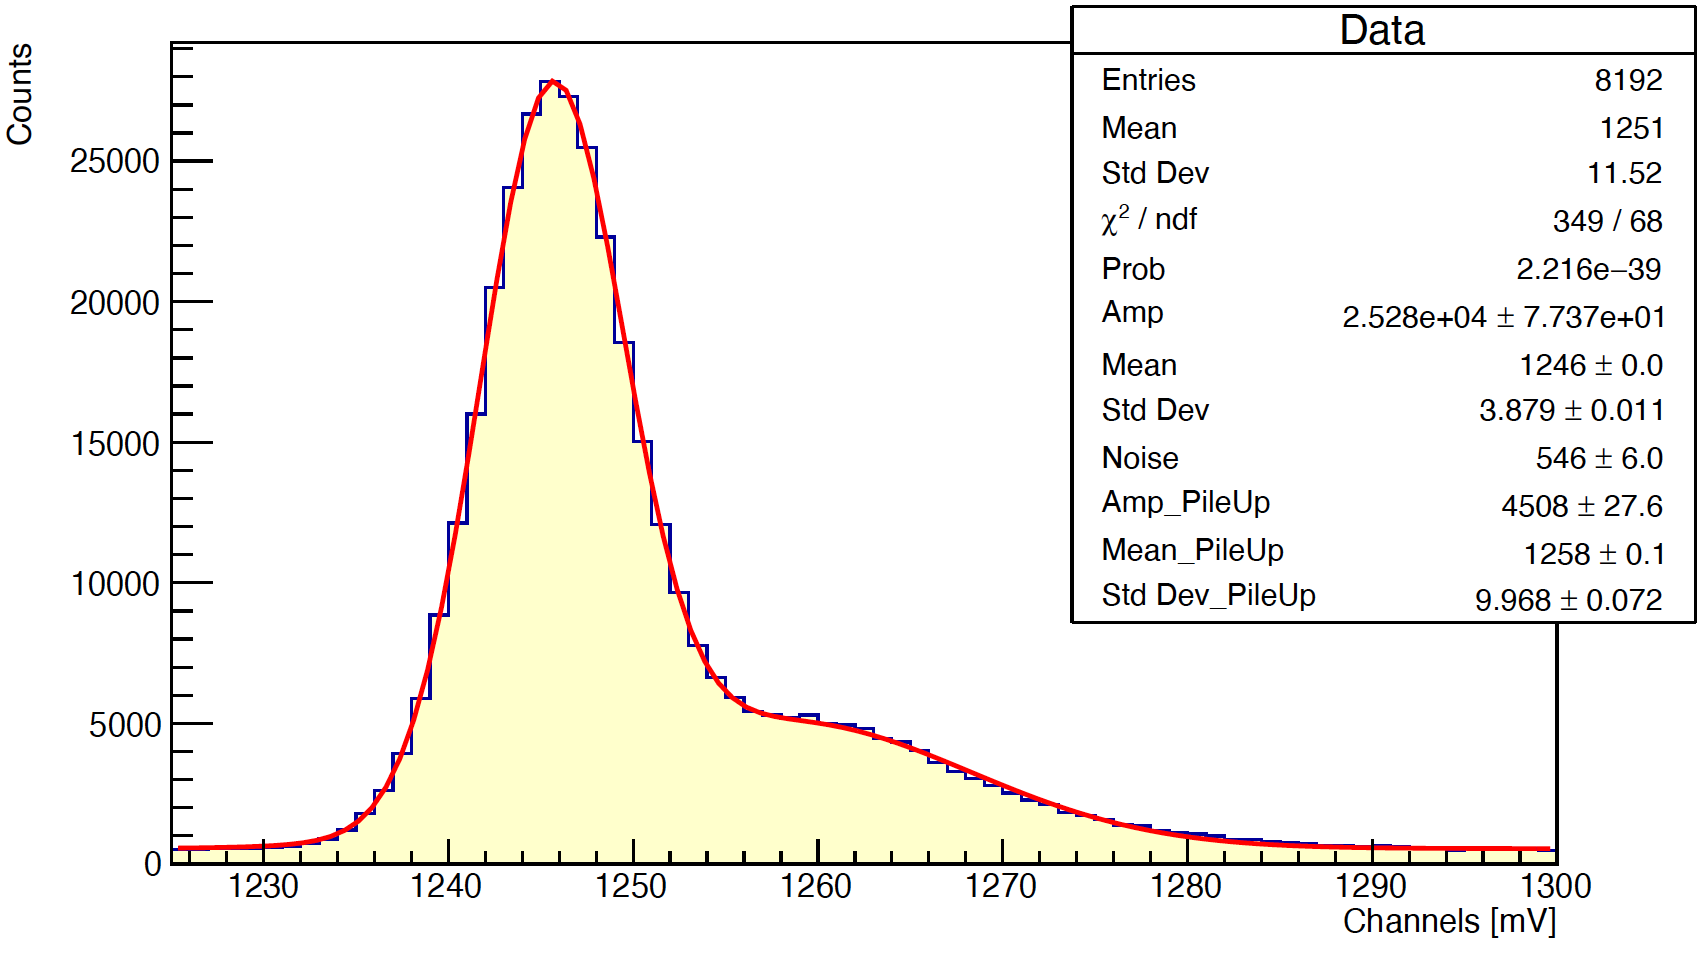
\includegraphics[scale=0.45]{appendice/spettri/NaPb1_1}
    \caption{Picco a 511 keV}
\end{figure}
\begin{figure}[H]
    \centering
    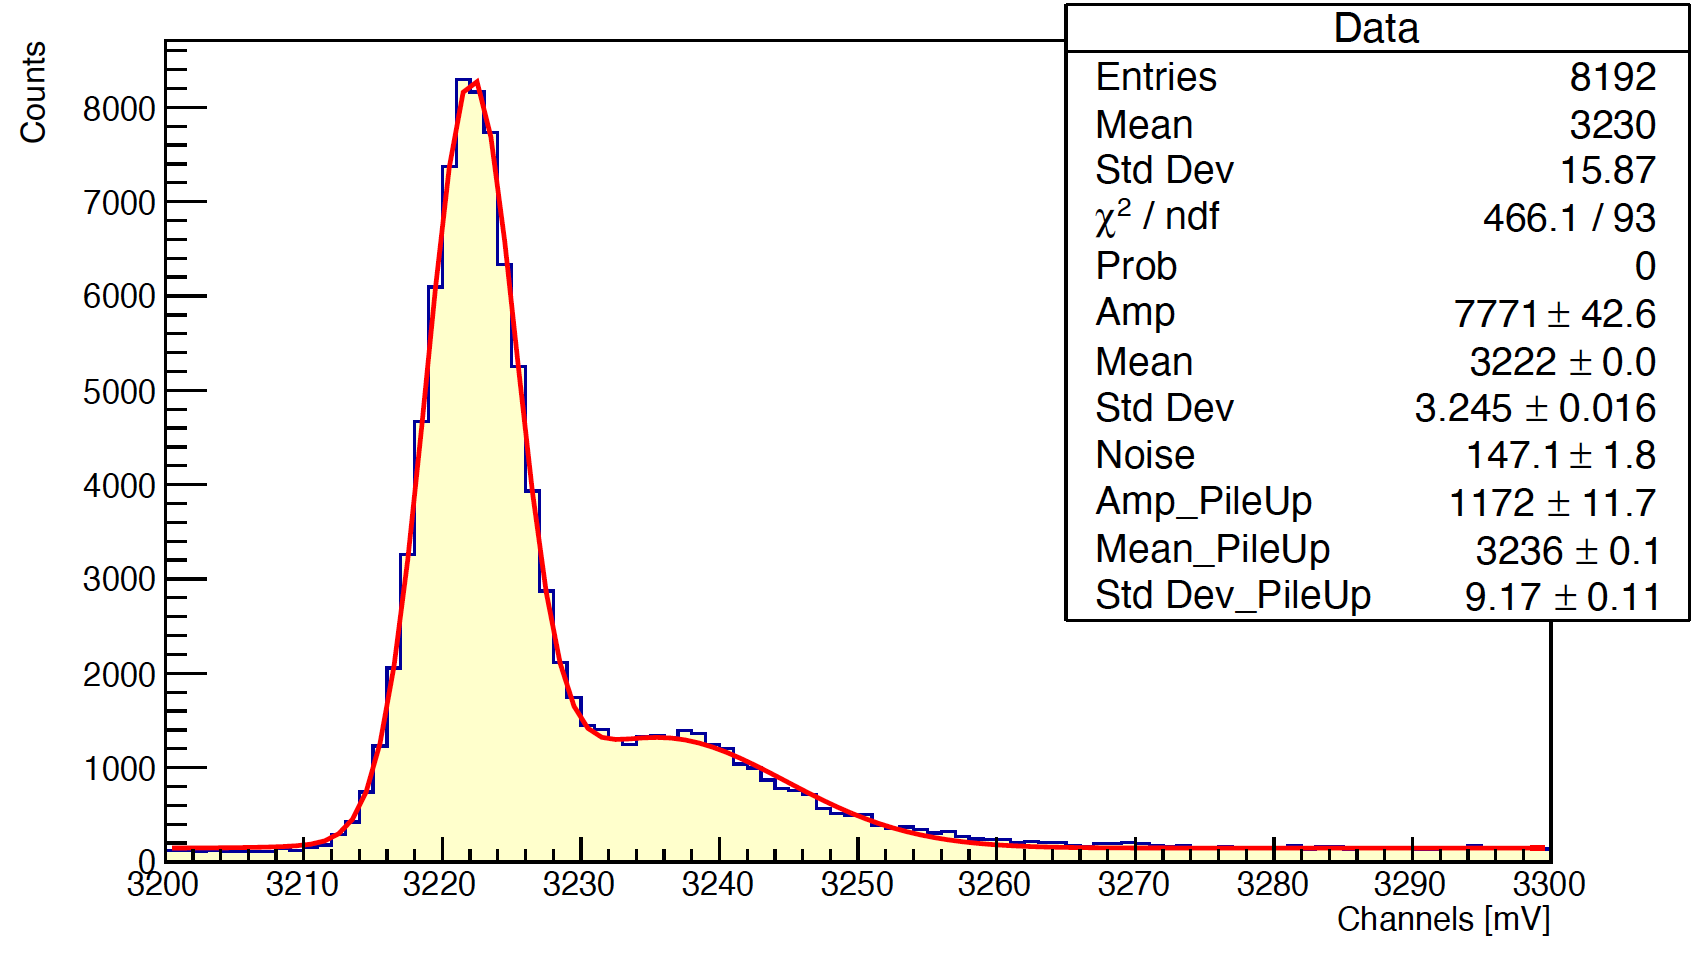
\includegraphics[scale=0.45]{appendice/spettri/NaPb2_1}
    \caption{Picco a 1274 keV}
\end{figure}
\begin{figure}[H]
    \centering
    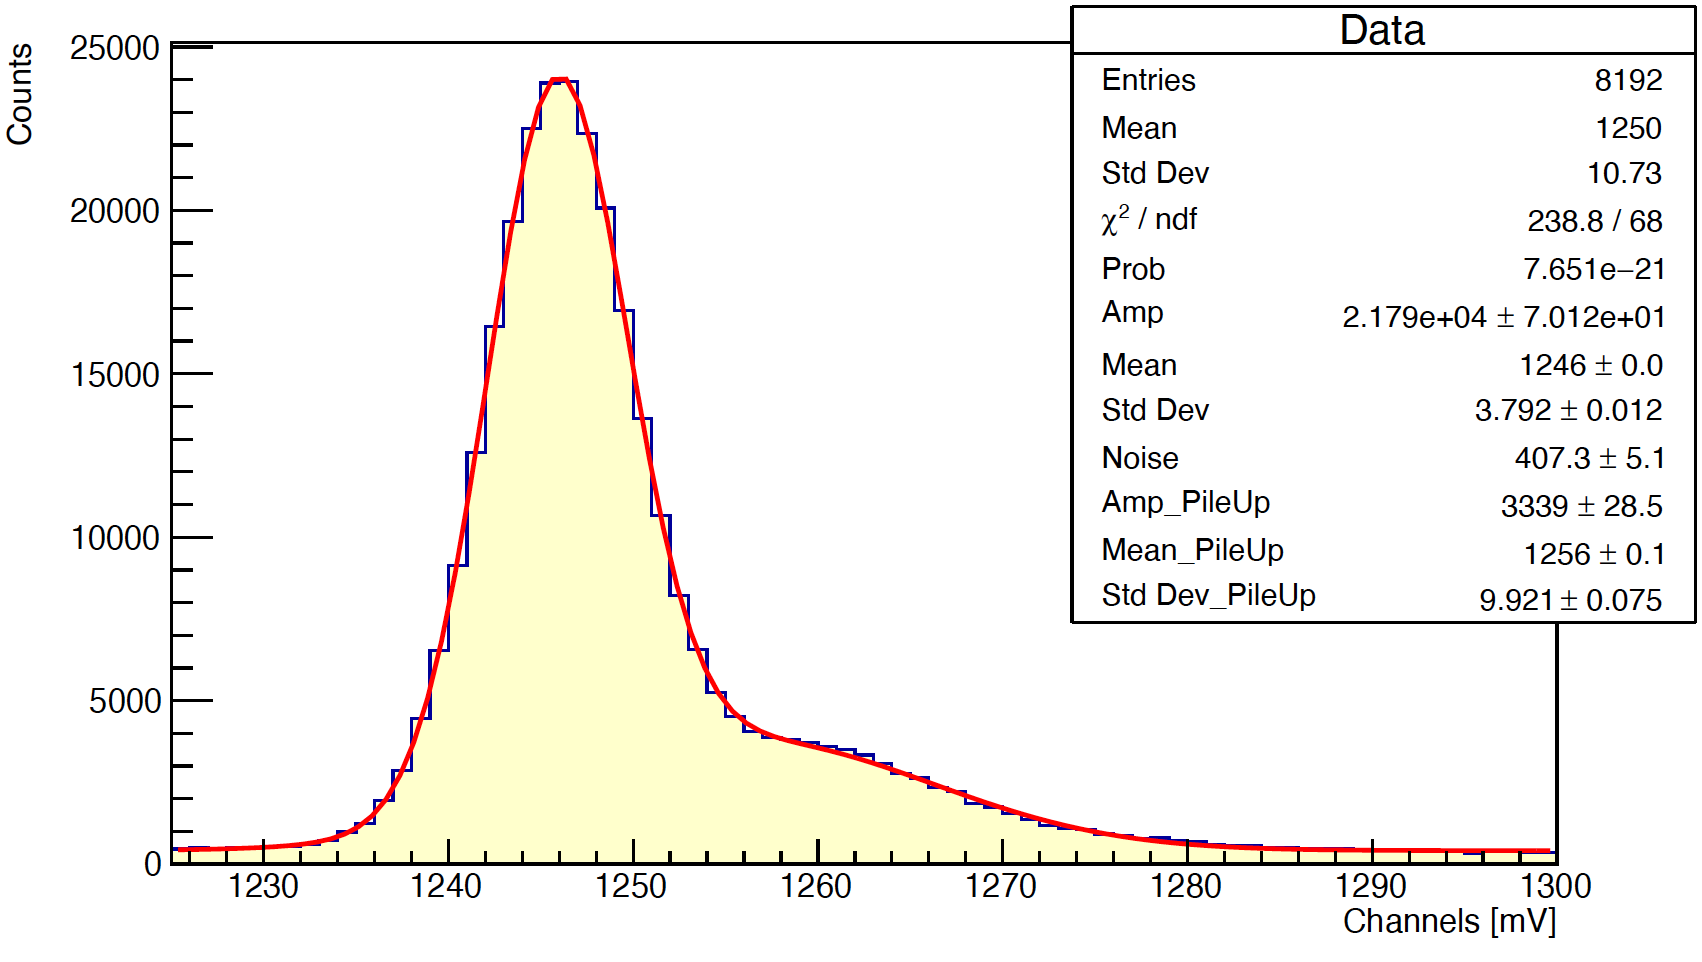
\includegraphics[scale=0.45]{appendice/spettri/NaPb1_21}
    \caption{Picco a 511 keV}
\end{figure}
\begin{figure}[H]
    \centering
    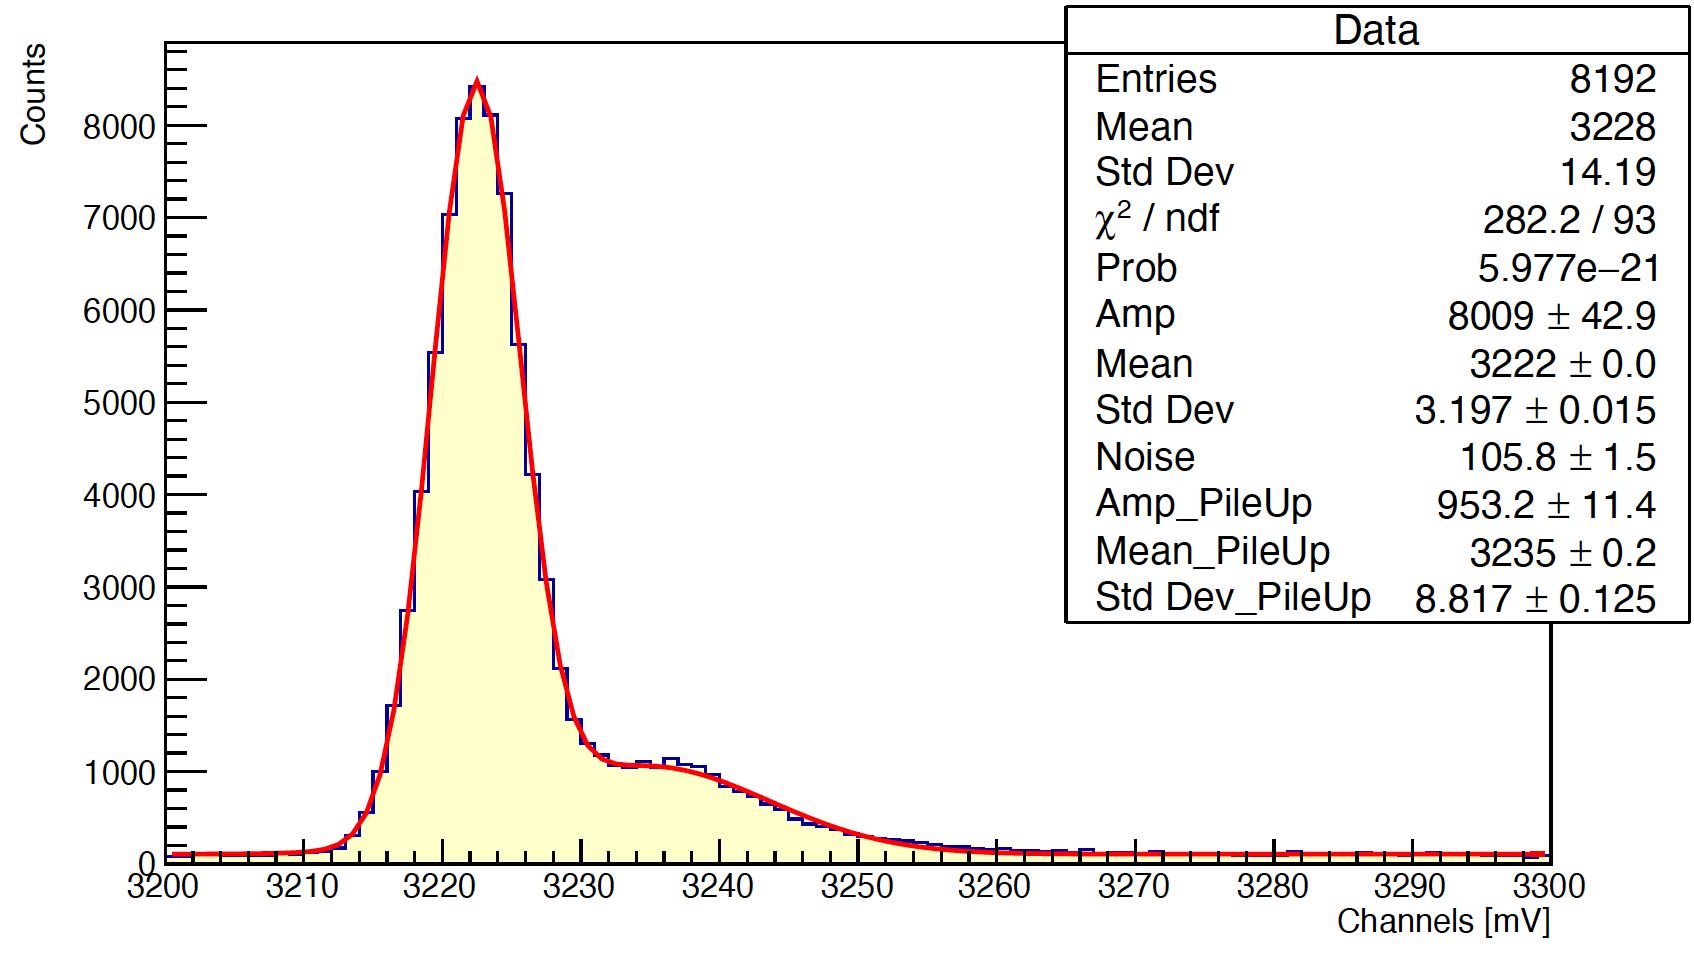
\includegraphics[scale=0.45]{appendice/spettri/NaPb2_21}
    \caption{Picco a 1274 keV}
\end{figure}
\begin{figure}[H]
    \centering
    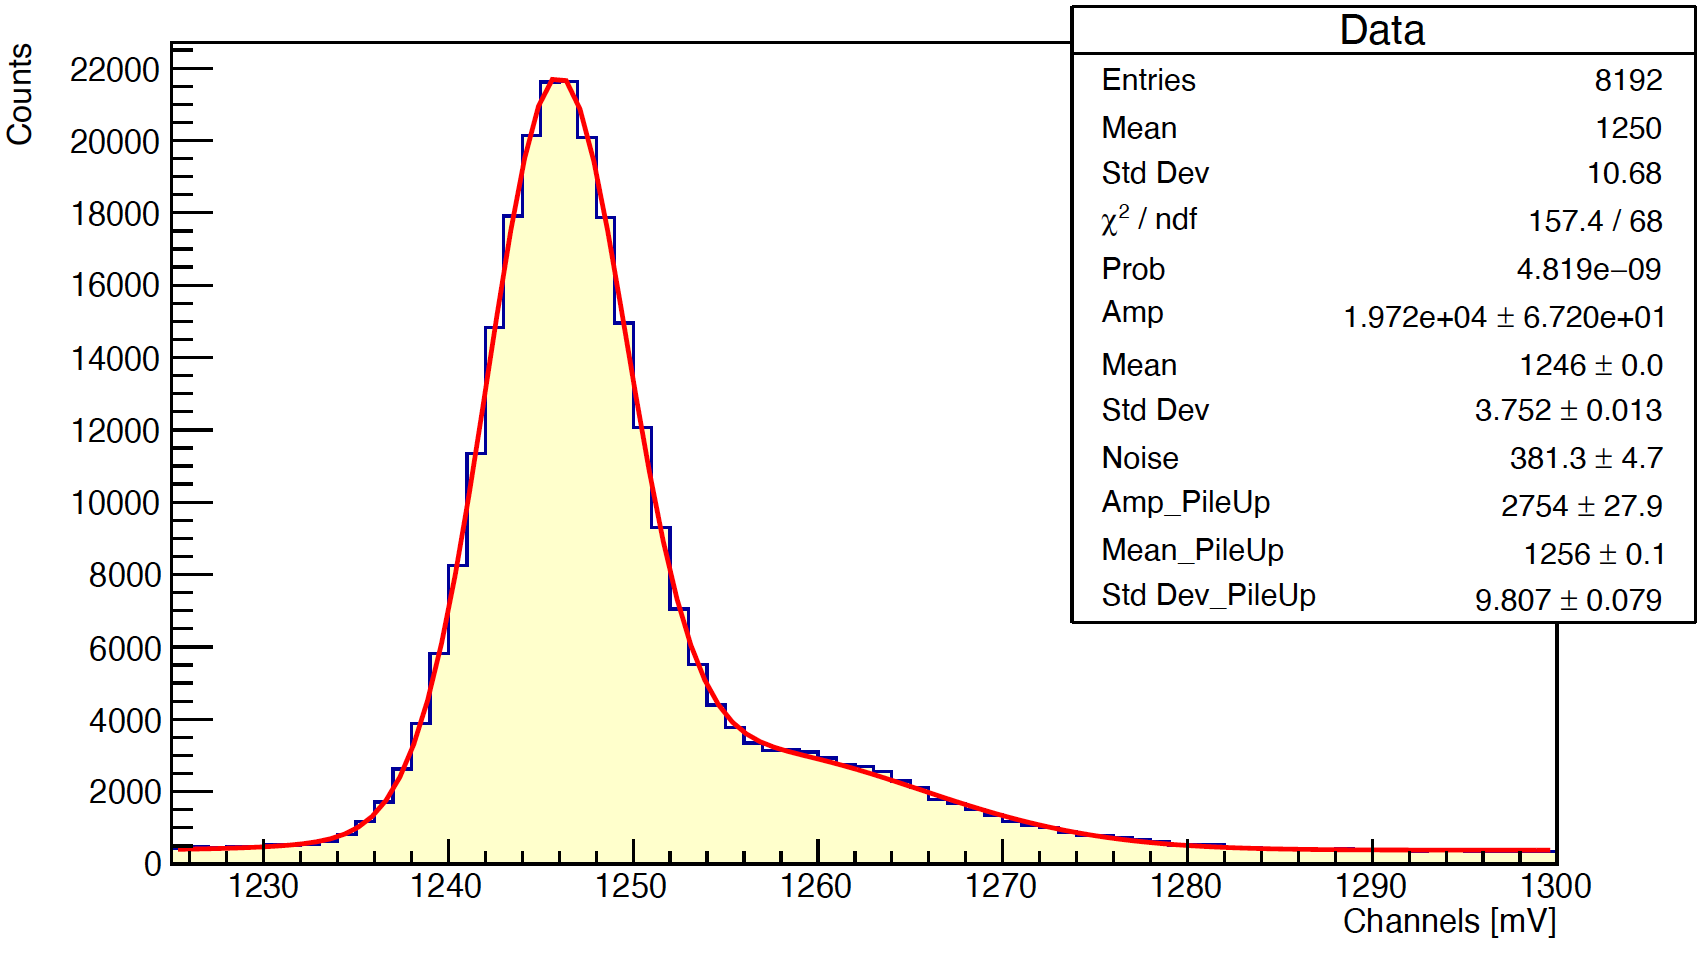
\includegraphics[scale=0.45]{appendice/spettri/NaPb1_33}
    \caption{Picco a 511 keV}
\end{figure}
\begin{figure}[H]
    \centering
    \includegraphics[scale=0.45]{appendice/spettri/NaPb2_33}
    \caption{Picco a 1274 keV}
\end{figure}
\begin{figure}[H]
    \centering
    \includegraphics[scale=0.45]{appendice/spettri/NaPb1_58}
    \caption{Picco a 511 keV}
\end{figure}
\begin{figure}[H]
    \centering
    \includegraphics[scale=0.45]{appendice/spettri/NaPb2_58}
    \caption{Picco a 1274 keV}
\end{figure}
\begin{figure}[H]
    \centering
    \includegraphics[scale=0.45]{appendice/spettri/NaPb1_108}
    \caption{Picco a 511 keV}
\end{figure}
\begin{figure}[H]
    \centering
    \includegraphics[scale=0.45]{appendice/spettri/NaPb2_108}
    \caption{Picco a 1274 keV}
\end{figure}

%%% Cobalto %%%
\subsection{Cobalto con acqua a 4, 8, 12, 16 e 20 cm di spessore}
\begin{figure}[H]
    \centering
    \includegraphics[scale=0.45]{appendice/spettri/CoA1_4}
    \caption{Picco a 1173 keV}
\end{figure}
\begin{figure}[H]
    \centering
    \includegraphics[scale=0.45]{appendice/spettri/CoA2_4}
    \caption{Picco a 1332 keV}
\end{figure}
\begin{figure}[H]
    \centering
    \includegraphics[scale=0.45]{appendice/spettri/CoA1_8}
    \caption{Picco a 1173 keV}
\end{figure}
\begin{figure}[H]
    \centering
    \includegraphics[scale=0.45]{appendice/spettri/CoA2_8}
    \caption{Picco a 1332 keV}
\end{figure}
\begin{figure}[H]
    \centering
    \includegraphics[scale=0.45]{appendice/spettri/CoA1_12}
    \caption{Picco a 1173 keV}
\end{figure}
\begin{figure}[H]
    \centering
    \includegraphics[scale=0.45]{appendice/spettri/CoA2_12}
    \caption{Picco a 1332 keV}
\end{figure}
\begin{figure}[H]
    \centering
    \includegraphics[scale=0.45]{appendice/spettri/CoA1_16}
    \caption{Picco a 1173 keV}
\end{figure}
\begin{figure}[H]
    \centering
    \includegraphics[scale=0.45]{appendice/spettri/CoA2_16}
    \caption{Picco a 1332 keV}
\end{figure}
\begin{figure}[H]
    \centering
    \includegraphics[scale=0.45]{appendice/spettri/CoA1_20}
    \caption{Picco a 1173 keV}
\end{figure}
\begin{figure}[H]
    \centering
    \includegraphics[scale=0.45]{appendice/spettri/CoA2_20}
    \caption{Picco a 1332 keV}
\end{figure}


%%% COBALTO %%%
\subsection{Cobalto con rame a 11, 22, 33, 44 e 54 cm di spessore}
\begin{figure}[H]
    \centering
    \includegraphics[scale=0.45]{appendice/spettri/CoCu1_11}
    \caption{Picco a 1173 keV}
\end{figure}
\begin{figure}[H]
    \centering
    \includegraphics[scale=0.45]{appendice/spettri/CoCu2_11}
    \caption{Picco a 1332 keV}
\end{figure}
\begin{figure}[H]
    \centering
    \includegraphics[scale=0.45]{appendice/spettri/CoCu1_22}
    \caption{Picco a 1173 keV}
\end{figure}
\begin{figure}[H]
    \centering
    \includegraphics[scale=0.45]{appendice/spettri/CoCu2_22}
    \caption{Picco a 1332 keV}
\end{figure}
\begin{figure}[H]
    \centering
    \includegraphics[scale=0.45]{appendice/spettri/CoCu1_33}
    \caption{Picco a 1173 keV}
\end{figure}
\begin{figure}[H]
    \centering
    \includegraphics[scale=0.45]{appendice/spettri/CoCu2_33}
    \caption{Picco a 1332 keV}
\end{figure}
\begin{figure}[H]
    \centering
    \includegraphics[scale=0.45]{appendice/spettri/CoCu1_44}
    \caption{Picco a 1173 keV}
\end{figure}
\begin{figure}[H]
    \centering
    \includegraphics[scale=0.45]{appendice/spettri/CoCu2_44}
    \caption{Picco a 1332 keV}
\end{figure}
\begin{figure}[H]
    \centering
    \includegraphics[scale=0.45]{appendice/spettri/CoCu1_54}
    \caption{Picco a 1173 keV}
\end{figure}
\begin{figure}[H]
    \centering
    \includegraphics[scale=0.45]{appendice/spettri/CoCu2_54}
    \caption{Picco a 1332 keV}
\end{figure}

\subsection{Cobalto con piombo a 1, 21, 33, 58 e 108 cm di spessore}
\begin{figure}[H]
    \centering
    \includegraphics[scale=0.45]{appendice/spettri/CoPb1_1}
    \caption{Picco a 1173 keV}
\end{figure}
\begin{figure}[H]
    \centering
    \includegraphics[scale=0.45]{appendice/spettri/CoPb2_1}
    \caption{Picco a 1332 keV}
\end{figure}
\begin{figure}[H]
    \centering
    \includegraphics[scale=0.45]{appendice/spettri/CoPb1_21}
    \caption{Picco a 1173 keV}
\end{figure}
\begin{figure}[H]
    \centering
    \includegraphics[scale=0.45]{appendice/spettri/CoPb2_21}
    \caption{Picco a 1332 keV}
\end{figure}
\begin{figure}[H]
    \centering
    \includegraphics[scale=0.45]{appendice/spettri/CoPb1_33}
    \caption{Picco a 1173 keV}
\end{figure}
\begin{figure}[H]
    \centering
    \includegraphics[scale=0.45]{appendice/spettri/CoPb2_33}
    \caption{Picco a 1332 keV}
\end{figure}
\begin{figure}[H]
    \centering
    \includegraphics[scale=0.45]{appendice/spettri/CoPb1_58}
    \caption{Picco a 1173 keV}
\end{figure}
\begin{figure}[H]
    \centering
    \includegraphics[scale=0.45]{appendice/spettri/CoPb2_58}
    \caption{Picco a 1332 keV}
\end{figure}
\begin{figure}[H]
    \centering
    \includegraphics[scale=0.45]{appendice/spettri/CoPb1_108}
    \caption{Picco a 1173 keV}
\end{figure}
\begin{figure}[H]
    \centering
    \includegraphics[scale=0.45]{appendice/spettri/CoPb2_108}
    \caption{Picco a 1332 keV}
\end{figure}

%%% Torio %%%
\subsection{Torio con acqua a 4, 8, 12, 16 e 20 cm di spessore}
\begin{figure}[H]
    \centering
    \includegraphics[scale=0.45]{appendice/spettri/ThA1_4}
    \caption{Picco a 238 keV}
\end{figure}
\begin{figure}[H]
    \centering
    \includegraphics[scale=0.45]{appendice/spettri/ThA2_4}
    \caption{Picco a 583 keV}
\end{figure}
\begin{figure}[H]
    \centering
    \includegraphics[scale=0.45]{appendice/spettri/ThA3_4}
    \caption{Picco a 2614 keV}
\end{figure}
\begin{figure}[H]
    \centering
    \includegraphics[scale=0.45]{appendice/spettri/ThA1_8}
    \caption{Picco a 238 keV}
\end{figure}
\begin{figure}[H]
    \centering
    \includegraphics[scale=0.45]{appendice/spettri/ThA2_8}
    \caption{Picco a 583 keV}
\end{figure}
\begin{figure}[H]
    \centering
    \includegraphics[scale=0.45]{appendice/spettri/ThA3_8}
    \caption{Picco a 2614 keV}
\end{figure}
\begin{figure}[H]
    \centering
    \includegraphics[scale=0.45]{appendice/spettri/ThA1_12}
    \caption{Picco a 238 keV}
\end{figure}
\begin{figure}[H]
    \centering
    \includegraphics[scale=0.45]{appendice/spettri/ThA2_12}
    \caption{Picco a 583 keV}
\end{figure}
\begin{figure}[H]
    \centering
    \includegraphics[scale=0.45]{appendice/spettri/ThA3_12}
    \caption{Picco a 2614 keV}
\end{figure}
\begin{figure}[H]
    \centering
    \includegraphics[scale=0.45]{appendice/spettri/ThA1_16}
    \caption{Picco a 238 keV}
\end{figure}
\begin{figure}[H]
    \centering
    \includegraphics[scale=0.45]{appendice/spettri/ThA2_16}
    \caption{Picco a 583 keV}
\end{figure}
\begin{figure}[H]
    \centering
    \includegraphics[scale=0.45]{appendice/spettri/ThA3_16}
    \caption{Picco a 2614 keV}
\end{figure}
\begin{figure}[H]
    \centering
    \includegraphics[scale=0.45]{appendice/spettri/ThA1_20}
    \caption{Picco a 238 keV}
\end{figure}
\begin{figure}[H]
    \centering
    \includegraphics[scale=0.45]{appendice/spettri/ThA2_20}
    \caption{Picco a 583 keV}
\end{figure}
\begin{figure}[H]
    \centering
    \includegraphics[scale=0.45]{appendice/spettri/ThA3_20}
    \caption{Picco a 2614 keV}
\end{figure}
\subsection{Torio con rame a 11, 22, 33, 44 e 54 cm di spessore}
\begin{figure}[H]
    \centering
    \includegraphics[scale=0.45]{appendice/spettri/ThCu1_11}
    \caption{Picco a 238 keV}
\end{figure}
\begin{figure}[H]
    \centering
    \includegraphics[scale=0.45]{appendice/spettri/ThCu2_11}
    \caption{Picco a 583 keV}
\end{figure}
\begin{figure}[H]
    \centering
    \includegraphics[scale=0.45]{appendice/spettri/ThCu3_11}
    \caption{Picco a 2614 keV}
\end{figure}
\begin{figure}[H]
    \centering
    \includegraphics[scale=0.45]{appendice/spettri/ThCu1_22}
    \caption{Picco a 238 keV}
\end{figure}
\begin{figure}[H]
    \centering
    \includegraphics[scale=0.45]{appendice/spettri/ThCu2_22}
    \caption{Picco a 583 keV}
\end{figure}
\begin{figure}[H]
    \centering
    \includegraphics[scale=0.45]{appendice/spettri/ThCu3_22}
    \caption{Picco a 2614 keV}
\end{figure}
\begin{figure}[H]
    \centering
    \includegraphics[scale=0.45]{appendice/spettri/ThCu1_33}
    \caption{Picco a 238 keV}
\end{figure}
\begin{figure}[H]
    \centering
    \includegraphics[scale=0.45]{appendice/spettri/ThCu2_33}
    \caption{Picco a 583 keV}
\end{figure}
\begin{figure}[H]
    \centering
    \includegraphics[scale=0.45]{appendice/spettri/ThCu3_33}
    \caption{Picco a 2614 keV}
\end{figure}
\begin{figure}[H]
    \centering
    \includegraphics[scale=0.45]{appendice/spettri/ThCu1_44}
    \caption{Picco a 238 keV}
\end{figure}
\begin{figure}[H]
    \centering
    \includegraphics[scale=0.45]{appendice/spettri/ThCu2_44}
    \caption{Picco a 583 keV}
\end{figure}
\begin{figure}[H]
    \centering
    \includegraphics[scale=0.45]{appendice/spettri/ThCu3_44}
    \caption{Picco a 2614 keV}
\end{figure}
\begin{figure}[H]
    \centering
    \includegraphics[scale=0.45]{appendice/spettri/ThCu1_54}
    \caption{Picco a 238 keV}
\end{figure}
\begin{figure}[H]
    \centering
    \includegraphics[scale=0.45]{appendice/spettri/ThCu2_54}
    \caption{Picco a 583 keV}
\end{figure}
\begin{figure}[H]
    \centering
    \includegraphics[scale=0.45]{appendice/spettri/ThCu3_54}
    \caption{Picco a 2614 keV}
\end{figure}
\subsection{Torio con piombo a 1, 21, 33, 58 e 108 cm di spessore}
\begin{figure}[H]
    \centering
    \includegraphics[scale=0.45]{appendice/spettri/ThPb1_1}
    \caption{Picco a 238 keV}
\end{figure}
\begin{figure}[H]
    \centering
    \includegraphics[scale=0.45]{appendice/spettri/ThPb2_1}
    \caption{Picco a 583 keV}
\end{figure}
\begin{figure}[H]
    \centering
    \includegraphics[scale=0.45]{appendice/spettri/ThPb3_1}
    \caption{Picco a 2614 keV}
\end{figure}
\begin{figure}[H]
    \centering
    \includegraphics[scale=0.45]{appendice/spettri/ThPb1_21}
    \caption{Picco a 238 keV}
\end{figure}
\begin{figure}[H]
    \centering
    \includegraphics[scale=0.45]{appendice/spettri/ThPb2_21}
    \caption{Picco a 583 keV}
\end{figure}
\begin{figure}[H]
    \centering
    \includegraphics[scale=0.45]{appendice/spettri/ThPb3_21}
    \caption{Picco a 2614 keV}
\end{figure}
\begin{figure}[H]
    \centering
    \includegraphics[scale=0.45]{appendice/spettri/ThPb1_33}
    \caption{Picco a 238 keV}
\end{figure}
\begin{figure}[H]
    \centering
    \includegraphics[scale=0.45]{appendice/spettri/ThPb2_33}
    \caption{Picco a 583 keV}
\end{figure}
\begin{figure}[H]
    \centering
    \includegraphics[scale=0.45]{appendice/spettri/ThPb3_33}
    \caption{Picco a 2614 keV}
\end{figure}
\begin{figure}[H]
    \centering
    \includegraphics[scale=0.45]{appendice/spettri/ThPb1_58}
    \caption{Picco a 238 keV}
\end{figure}
\begin{figure}[H]
    \centering
    \includegraphics[scale=0.45]{appendice/spettri/ThPb2_58}
    \caption{Picco a 583 keV}
\end{figure}
\begin{figure}[H]
    \centering
    \includegraphics[scale=0.45]{appendice/spettri/ThPb3_58}
    \caption{Picco a 2614 keV}
\end{figure}
\begin{figure}[H]
    \centering
    \includegraphics[scale=0.45]{appendice/spettri/ThPb2_108}
    \caption{Picco a 583 keV}
\end{figure}
\begin{figure}[H]
    \centering
    \includegraphics[scale=0.45]{appendice/spettri/ThPb3_108}
    \caption{Picco a 2614 keV}
\end{figure}
\subsection{Picco a 1460 keV sodio con acqua a 4, 8, 12, 16, 20 cm di spessore}
\begin{figure}[H]
    \centering
    \includegraphics[scale=0.45]{appendice/spettri/NaA_1460_4}
\end{figure}
\begin{figure}[H]
    \centering
    \includegraphics[scale=0.45]{appendice/spettri/NaA_1460_8}
\end{figure}
\begin{figure}[H]
    \centering
    \includegraphics[scale=0.45]{appendice/spettri/NaA_1460_12}
\end{figure}
\begin{figure}[H]
    \centering
    \includegraphics[scale=0.45]{appendice/spettri/NaA_1460_16}
\end{figure}
\begin{figure}[H]
    \centering
    \includegraphics[scale=0.45]{appendice/spettri/NaA_1460_20}
\end{figure}

\subsection{Picco a 1460 keV cobalto con acqua a 4, 8, 12, 16, 20 cm di spessore}
\begin{figure}[H]
    \centering
    \includegraphics[scale=0.45]{appendice/spettri/CoA_1460_4}
\end{figure}
\begin{figure}[H]
    \centering
    \includegraphics[scale=0.45]{appendice/spettri/CoA_1460_8}
\end{figure}
\begin{figure}[H]
    \centering
    \includegraphics[scale=0.45]{appendice/spettri/CoA_1460_12}
\end{figure}
\begin{figure}[H]
    \centering
    \includegraphics[scale=0.45]{appendice/spettri/CoA_1460_16}
\end{figure}
\begin{figure}[H]
    \centering
    \includegraphics[scale=0.45]{appendice/spettri/CoA_1460_20}
\end{figure}

\subsection{Picco a 1460 keV torio con acqua a 4, 8, 12, 16, 20 cm di spessore}
\begin{figure}[H]
    \centering
    \includegraphics[scale=0.45]{appendice/spettri/ThA_1460_4}
\end{figure}
\begin{figure}[H]
    \centering
    \includegraphics[scale=0.45]{appendice/spettri/ThA_1460_8}
\end{figure}
\begin{figure}[H]
    \centering
    \includegraphics[scale=0.45]{appendice/spettri/ThA_1460_12}
\end{figure}
\begin{figure}[H]
    \centering
    \includegraphics[scale=0.45]{appendice/spettri/ThA_1460_16}
\end{figure}
\begin{figure}[H]
    \centering
    \includegraphics[scale=0.45]{appendice/spettri/ThA_1460_20}
\end{figure}
\end{document}